\begin{frame}
  \frametitle{Example}
  \begin{onlyenv}<1>
    Consider the following mapping $x \rightarrow y$
    \begin{center}
      \scalebox{0.5}{
        %% Creator: Matplotlib, PGF backend
%%
%% To include the figure in your LaTeX document, write
%%   \input{<filename>.pgf}
%%
%% Make sure the required packages are loaded in your preamble
%%   \usepackage{pgf}
%%
%% Figures using additional raster images can only be included by \input if
%% they are in the same directory as the main LaTeX file. For loading figures
%% from other directories you can use the `import` package
%%   \usepackage{import}
%% and then include the figures with
%%   \import{<path to file>}{<filename>.pgf}
%%
%% Matplotlib used the following preamble
%%   \usepackage{fontspec}
%%   \setmainfont{DejaVuSerif.ttf}[Path=/home/diou/miniconda3/envs/ml/lib/python3.8/site-packages/matplotlib/mpl-data/fonts/ttf/]
%%   \setsansfont{DejaVuSans.ttf}[Path=/home/diou/miniconda3/envs/ml/lib/python3.8/site-packages/matplotlib/mpl-data/fonts/ttf/]
%%   \setmonofont{DejaVuSansMono.ttf}[Path=/home/diou/miniconda3/envs/ml/lib/python3.8/site-packages/matplotlib/mpl-data/fonts/ttf/]
%%
\begingroup%
\makeatletter%
\begin{pgfpicture}%
\pgfpathrectangle{\pgfpointorigin}{\pgfqpoint{6.400000in}{4.800000in}}%
\pgfusepath{use as bounding box, clip}%
\begin{pgfscope}%
\pgfsetbuttcap%
\pgfsetmiterjoin%
\definecolor{currentfill}{rgb}{1.000000,1.000000,1.000000}%
\pgfsetfillcolor{currentfill}%
\pgfsetlinewidth{0.000000pt}%
\definecolor{currentstroke}{rgb}{1.000000,1.000000,1.000000}%
\pgfsetstrokecolor{currentstroke}%
\pgfsetdash{}{0pt}%
\pgfpathmoveto{\pgfqpoint{0.000000in}{0.000000in}}%
\pgfpathlineto{\pgfqpoint{6.400000in}{0.000000in}}%
\pgfpathlineto{\pgfqpoint{6.400000in}{4.800000in}}%
\pgfpathlineto{\pgfqpoint{0.000000in}{4.800000in}}%
\pgfpathclose%
\pgfusepath{fill}%
\end{pgfscope}%
\begin{pgfscope}%
\pgfsetbuttcap%
\pgfsetmiterjoin%
\definecolor{currentfill}{rgb}{1.000000,1.000000,1.000000}%
\pgfsetfillcolor{currentfill}%
\pgfsetlinewidth{0.000000pt}%
\definecolor{currentstroke}{rgb}{0.000000,0.000000,0.000000}%
\pgfsetstrokecolor{currentstroke}%
\pgfsetstrokeopacity{0.000000}%
\pgfsetdash{}{0pt}%
\pgfpathmoveto{\pgfqpoint{0.800000in}{0.528000in}}%
\pgfpathlineto{\pgfqpoint{5.760000in}{0.528000in}}%
\pgfpathlineto{\pgfqpoint{5.760000in}{4.224000in}}%
\pgfpathlineto{\pgfqpoint{0.800000in}{4.224000in}}%
\pgfpathclose%
\pgfusepath{fill}%
\end{pgfscope}%
\begin{pgfscope}%
\pgfpathrectangle{\pgfqpoint{0.800000in}{0.528000in}}{\pgfqpoint{4.960000in}{3.696000in}}%
\pgfusepath{clip}%
\pgfsetrectcap%
\pgfsetroundjoin%
\pgfsetlinewidth{0.803000pt}%
\definecolor{currentstroke}{rgb}{0.690196,0.690196,0.690196}%
\pgfsetstrokecolor{currentstroke}%
\pgfsetdash{}{0pt}%
\pgfpathmoveto{\pgfqpoint{1.025455in}{0.528000in}}%
\pgfpathlineto{\pgfqpoint{1.025455in}{4.224000in}}%
\pgfusepath{stroke}%
\end{pgfscope}%
\begin{pgfscope}%
\pgfsetbuttcap%
\pgfsetroundjoin%
\definecolor{currentfill}{rgb}{0.000000,0.000000,0.000000}%
\pgfsetfillcolor{currentfill}%
\pgfsetlinewidth{0.803000pt}%
\definecolor{currentstroke}{rgb}{0.000000,0.000000,0.000000}%
\pgfsetstrokecolor{currentstroke}%
\pgfsetdash{}{0pt}%
\pgfsys@defobject{currentmarker}{\pgfqpoint{0.000000in}{-0.048611in}}{\pgfqpoint{0.000000in}{0.000000in}}{%
\pgfpathmoveto{\pgfqpoint{0.000000in}{0.000000in}}%
\pgfpathlineto{\pgfqpoint{0.000000in}{-0.048611in}}%
\pgfusepath{stroke,fill}%
}%
\begin{pgfscope}%
\pgfsys@transformshift{1.025455in}{0.528000in}%
\pgfsys@useobject{currentmarker}{}%
\end{pgfscope}%
\end{pgfscope}%
\begin{pgfscope}%
\definecolor{textcolor}{rgb}{0.000000,0.000000,0.000000}%
\pgfsetstrokecolor{textcolor}%
\pgfsetfillcolor{textcolor}%
\pgftext[x=1.025455in,y=0.430778in,,top]{\color{textcolor}\sffamily\fontsize{10.000000}{12.000000}\selectfont 0.0}%
\end{pgfscope}%
\begin{pgfscope}%
\pgfpathrectangle{\pgfqpoint{0.800000in}{0.528000in}}{\pgfqpoint{4.960000in}{3.696000in}}%
\pgfusepath{clip}%
\pgfsetrectcap%
\pgfsetroundjoin%
\pgfsetlinewidth{0.803000pt}%
\definecolor{currentstroke}{rgb}{0.690196,0.690196,0.690196}%
\pgfsetstrokecolor{currentstroke}%
\pgfsetdash{}{0pt}%
\pgfpathmoveto{\pgfqpoint{1.927273in}{0.528000in}}%
\pgfpathlineto{\pgfqpoint{1.927273in}{4.224000in}}%
\pgfusepath{stroke}%
\end{pgfscope}%
\begin{pgfscope}%
\pgfsetbuttcap%
\pgfsetroundjoin%
\definecolor{currentfill}{rgb}{0.000000,0.000000,0.000000}%
\pgfsetfillcolor{currentfill}%
\pgfsetlinewidth{0.803000pt}%
\definecolor{currentstroke}{rgb}{0.000000,0.000000,0.000000}%
\pgfsetstrokecolor{currentstroke}%
\pgfsetdash{}{0pt}%
\pgfsys@defobject{currentmarker}{\pgfqpoint{0.000000in}{-0.048611in}}{\pgfqpoint{0.000000in}{0.000000in}}{%
\pgfpathmoveto{\pgfqpoint{0.000000in}{0.000000in}}%
\pgfpathlineto{\pgfqpoint{0.000000in}{-0.048611in}}%
\pgfusepath{stroke,fill}%
}%
\begin{pgfscope}%
\pgfsys@transformshift{1.927273in}{0.528000in}%
\pgfsys@useobject{currentmarker}{}%
\end{pgfscope}%
\end{pgfscope}%
\begin{pgfscope}%
\definecolor{textcolor}{rgb}{0.000000,0.000000,0.000000}%
\pgfsetstrokecolor{textcolor}%
\pgfsetfillcolor{textcolor}%
\pgftext[x=1.927273in,y=0.430778in,,top]{\color{textcolor}\sffamily\fontsize{10.000000}{12.000000}\selectfont 0.5}%
\end{pgfscope}%
\begin{pgfscope}%
\pgfpathrectangle{\pgfqpoint{0.800000in}{0.528000in}}{\pgfqpoint{4.960000in}{3.696000in}}%
\pgfusepath{clip}%
\pgfsetrectcap%
\pgfsetroundjoin%
\pgfsetlinewidth{0.803000pt}%
\definecolor{currentstroke}{rgb}{0.690196,0.690196,0.690196}%
\pgfsetstrokecolor{currentstroke}%
\pgfsetdash{}{0pt}%
\pgfpathmoveto{\pgfqpoint{2.829091in}{0.528000in}}%
\pgfpathlineto{\pgfqpoint{2.829091in}{4.224000in}}%
\pgfusepath{stroke}%
\end{pgfscope}%
\begin{pgfscope}%
\pgfsetbuttcap%
\pgfsetroundjoin%
\definecolor{currentfill}{rgb}{0.000000,0.000000,0.000000}%
\pgfsetfillcolor{currentfill}%
\pgfsetlinewidth{0.803000pt}%
\definecolor{currentstroke}{rgb}{0.000000,0.000000,0.000000}%
\pgfsetstrokecolor{currentstroke}%
\pgfsetdash{}{0pt}%
\pgfsys@defobject{currentmarker}{\pgfqpoint{0.000000in}{-0.048611in}}{\pgfqpoint{0.000000in}{0.000000in}}{%
\pgfpathmoveto{\pgfqpoint{0.000000in}{0.000000in}}%
\pgfpathlineto{\pgfqpoint{0.000000in}{-0.048611in}}%
\pgfusepath{stroke,fill}%
}%
\begin{pgfscope}%
\pgfsys@transformshift{2.829091in}{0.528000in}%
\pgfsys@useobject{currentmarker}{}%
\end{pgfscope}%
\end{pgfscope}%
\begin{pgfscope}%
\definecolor{textcolor}{rgb}{0.000000,0.000000,0.000000}%
\pgfsetstrokecolor{textcolor}%
\pgfsetfillcolor{textcolor}%
\pgftext[x=2.829091in,y=0.430778in,,top]{\color{textcolor}\sffamily\fontsize{10.000000}{12.000000}\selectfont 1.0}%
\end{pgfscope}%
\begin{pgfscope}%
\pgfpathrectangle{\pgfqpoint{0.800000in}{0.528000in}}{\pgfqpoint{4.960000in}{3.696000in}}%
\pgfusepath{clip}%
\pgfsetrectcap%
\pgfsetroundjoin%
\pgfsetlinewidth{0.803000pt}%
\definecolor{currentstroke}{rgb}{0.690196,0.690196,0.690196}%
\pgfsetstrokecolor{currentstroke}%
\pgfsetdash{}{0pt}%
\pgfpathmoveto{\pgfqpoint{3.730909in}{0.528000in}}%
\pgfpathlineto{\pgfqpoint{3.730909in}{4.224000in}}%
\pgfusepath{stroke}%
\end{pgfscope}%
\begin{pgfscope}%
\pgfsetbuttcap%
\pgfsetroundjoin%
\definecolor{currentfill}{rgb}{0.000000,0.000000,0.000000}%
\pgfsetfillcolor{currentfill}%
\pgfsetlinewidth{0.803000pt}%
\definecolor{currentstroke}{rgb}{0.000000,0.000000,0.000000}%
\pgfsetstrokecolor{currentstroke}%
\pgfsetdash{}{0pt}%
\pgfsys@defobject{currentmarker}{\pgfqpoint{0.000000in}{-0.048611in}}{\pgfqpoint{0.000000in}{0.000000in}}{%
\pgfpathmoveto{\pgfqpoint{0.000000in}{0.000000in}}%
\pgfpathlineto{\pgfqpoint{0.000000in}{-0.048611in}}%
\pgfusepath{stroke,fill}%
}%
\begin{pgfscope}%
\pgfsys@transformshift{3.730909in}{0.528000in}%
\pgfsys@useobject{currentmarker}{}%
\end{pgfscope}%
\end{pgfscope}%
\begin{pgfscope}%
\definecolor{textcolor}{rgb}{0.000000,0.000000,0.000000}%
\pgfsetstrokecolor{textcolor}%
\pgfsetfillcolor{textcolor}%
\pgftext[x=3.730909in,y=0.430778in,,top]{\color{textcolor}\sffamily\fontsize{10.000000}{12.000000}\selectfont 1.5}%
\end{pgfscope}%
\begin{pgfscope}%
\pgfpathrectangle{\pgfqpoint{0.800000in}{0.528000in}}{\pgfqpoint{4.960000in}{3.696000in}}%
\pgfusepath{clip}%
\pgfsetrectcap%
\pgfsetroundjoin%
\pgfsetlinewidth{0.803000pt}%
\definecolor{currentstroke}{rgb}{0.690196,0.690196,0.690196}%
\pgfsetstrokecolor{currentstroke}%
\pgfsetdash{}{0pt}%
\pgfpathmoveto{\pgfqpoint{4.632727in}{0.528000in}}%
\pgfpathlineto{\pgfqpoint{4.632727in}{4.224000in}}%
\pgfusepath{stroke}%
\end{pgfscope}%
\begin{pgfscope}%
\pgfsetbuttcap%
\pgfsetroundjoin%
\definecolor{currentfill}{rgb}{0.000000,0.000000,0.000000}%
\pgfsetfillcolor{currentfill}%
\pgfsetlinewidth{0.803000pt}%
\definecolor{currentstroke}{rgb}{0.000000,0.000000,0.000000}%
\pgfsetstrokecolor{currentstroke}%
\pgfsetdash{}{0pt}%
\pgfsys@defobject{currentmarker}{\pgfqpoint{0.000000in}{-0.048611in}}{\pgfqpoint{0.000000in}{0.000000in}}{%
\pgfpathmoveto{\pgfqpoint{0.000000in}{0.000000in}}%
\pgfpathlineto{\pgfqpoint{0.000000in}{-0.048611in}}%
\pgfusepath{stroke,fill}%
}%
\begin{pgfscope}%
\pgfsys@transformshift{4.632727in}{0.528000in}%
\pgfsys@useobject{currentmarker}{}%
\end{pgfscope}%
\end{pgfscope}%
\begin{pgfscope}%
\definecolor{textcolor}{rgb}{0.000000,0.000000,0.000000}%
\pgfsetstrokecolor{textcolor}%
\pgfsetfillcolor{textcolor}%
\pgftext[x=4.632727in,y=0.430778in,,top]{\color{textcolor}\sffamily\fontsize{10.000000}{12.000000}\selectfont 2.0}%
\end{pgfscope}%
\begin{pgfscope}%
\pgfpathrectangle{\pgfqpoint{0.800000in}{0.528000in}}{\pgfqpoint{4.960000in}{3.696000in}}%
\pgfusepath{clip}%
\pgfsetrectcap%
\pgfsetroundjoin%
\pgfsetlinewidth{0.803000pt}%
\definecolor{currentstroke}{rgb}{0.690196,0.690196,0.690196}%
\pgfsetstrokecolor{currentstroke}%
\pgfsetdash{}{0pt}%
\pgfpathmoveto{\pgfqpoint{5.534545in}{0.528000in}}%
\pgfpathlineto{\pgfqpoint{5.534545in}{4.224000in}}%
\pgfusepath{stroke}%
\end{pgfscope}%
\begin{pgfscope}%
\pgfsetbuttcap%
\pgfsetroundjoin%
\definecolor{currentfill}{rgb}{0.000000,0.000000,0.000000}%
\pgfsetfillcolor{currentfill}%
\pgfsetlinewidth{0.803000pt}%
\definecolor{currentstroke}{rgb}{0.000000,0.000000,0.000000}%
\pgfsetstrokecolor{currentstroke}%
\pgfsetdash{}{0pt}%
\pgfsys@defobject{currentmarker}{\pgfqpoint{0.000000in}{-0.048611in}}{\pgfqpoint{0.000000in}{0.000000in}}{%
\pgfpathmoveto{\pgfqpoint{0.000000in}{0.000000in}}%
\pgfpathlineto{\pgfqpoint{0.000000in}{-0.048611in}}%
\pgfusepath{stroke,fill}%
}%
\begin{pgfscope}%
\pgfsys@transformshift{5.534545in}{0.528000in}%
\pgfsys@useobject{currentmarker}{}%
\end{pgfscope}%
\end{pgfscope}%
\begin{pgfscope}%
\definecolor{textcolor}{rgb}{0.000000,0.000000,0.000000}%
\pgfsetstrokecolor{textcolor}%
\pgfsetfillcolor{textcolor}%
\pgftext[x=5.534545in,y=0.430778in,,top]{\color{textcolor}\sffamily\fontsize{10.000000}{12.000000}\selectfont 2.5}%
\end{pgfscope}%
\begin{pgfscope}%
\definecolor{textcolor}{rgb}{0.000000,0.000000,0.000000}%
\pgfsetstrokecolor{textcolor}%
\pgfsetfillcolor{textcolor}%
\pgftext[x=3.280000in,y=0.240809in,,top]{\color{textcolor}\sffamily\fontsize{10.000000}{12.000000}\selectfont x}%
\end{pgfscope}%
\begin{pgfscope}%
\pgfpathrectangle{\pgfqpoint{0.800000in}{0.528000in}}{\pgfqpoint{4.960000in}{3.696000in}}%
\pgfusepath{clip}%
\pgfsetrectcap%
\pgfsetroundjoin%
\pgfsetlinewidth{0.803000pt}%
\definecolor{currentstroke}{rgb}{0.690196,0.690196,0.690196}%
\pgfsetstrokecolor{currentstroke}%
\pgfsetdash{}{0pt}%
\pgfpathmoveto{\pgfqpoint{0.800000in}{0.864000in}}%
\pgfpathlineto{\pgfqpoint{5.760000in}{0.864000in}}%
\pgfusepath{stroke}%
\end{pgfscope}%
\begin{pgfscope}%
\pgfsetbuttcap%
\pgfsetroundjoin%
\definecolor{currentfill}{rgb}{0.000000,0.000000,0.000000}%
\pgfsetfillcolor{currentfill}%
\pgfsetlinewidth{0.803000pt}%
\definecolor{currentstroke}{rgb}{0.000000,0.000000,0.000000}%
\pgfsetstrokecolor{currentstroke}%
\pgfsetdash{}{0pt}%
\pgfsys@defobject{currentmarker}{\pgfqpoint{-0.048611in}{0.000000in}}{\pgfqpoint{0.000000in}{0.000000in}}{%
\pgfpathmoveto{\pgfqpoint{0.000000in}{0.000000in}}%
\pgfpathlineto{\pgfqpoint{-0.048611in}{0.000000in}}%
\pgfusepath{stroke,fill}%
}%
\begin{pgfscope}%
\pgfsys@transformshift{0.800000in}{0.864000in}%
\pgfsys@useobject{currentmarker}{}%
\end{pgfscope}%
\end{pgfscope}%
\begin{pgfscope}%
\definecolor{textcolor}{rgb}{0.000000,0.000000,0.000000}%
\pgfsetstrokecolor{textcolor}%
\pgfsetfillcolor{textcolor}%
\pgftext[x=0.481898in,y=0.811238in,left,base]{\color{textcolor}\sffamily\fontsize{10.000000}{12.000000}\selectfont 0.6}%
\end{pgfscope}%
\begin{pgfscope}%
\pgfpathrectangle{\pgfqpoint{0.800000in}{0.528000in}}{\pgfqpoint{4.960000in}{3.696000in}}%
\pgfusepath{clip}%
\pgfsetrectcap%
\pgfsetroundjoin%
\pgfsetlinewidth{0.803000pt}%
\definecolor{currentstroke}{rgb}{0.690196,0.690196,0.690196}%
\pgfsetstrokecolor{currentstroke}%
\pgfsetdash{}{0pt}%
\pgfpathmoveto{\pgfqpoint{0.800000in}{1.536000in}}%
\pgfpathlineto{\pgfqpoint{5.760000in}{1.536000in}}%
\pgfusepath{stroke}%
\end{pgfscope}%
\begin{pgfscope}%
\pgfsetbuttcap%
\pgfsetroundjoin%
\definecolor{currentfill}{rgb}{0.000000,0.000000,0.000000}%
\pgfsetfillcolor{currentfill}%
\pgfsetlinewidth{0.803000pt}%
\definecolor{currentstroke}{rgb}{0.000000,0.000000,0.000000}%
\pgfsetstrokecolor{currentstroke}%
\pgfsetdash{}{0pt}%
\pgfsys@defobject{currentmarker}{\pgfqpoint{-0.048611in}{0.000000in}}{\pgfqpoint{0.000000in}{0.000000in}}{%
\pgfpathmoveto{\pgfqpoint{0.000000in}{0.000000in}}%
\pgfpathlineto{\pgfqpoint{-0.048611in}{0.000000in}}%
\pgfusepath{stroke,fill}%
}%
\begin{pgfscope}%
\pgfsys@transformshift{0.800000in}{1.536000in}%
\pgfsys@useobject{currentmarker}{}%
\end{pgfscope}%
\end{pgfscope}%
\begin{pgfscope}%
\definecolor{textcolor}{rgb}{0.000000,0.000000,0.000000}%
\pgfsetstrokecolor{textcolor}%
\pgfsetfillcolor{textcolor}%
\pgftext[x=0.481898in,y=1.483238in,left,base]{\color{textcolor}\sffamily\fontsize{10.000000}{12.000000}\selectfont 0.8}%
\end{pgfscope}%
\begin{pgfscope}%
\pgfpathrectangle{\pgfqpoint{0.800000in}{0.528000in}}{\pgfqpoint{4.960000in}{3.696000in}}%
\pgfusepath{clip}%
\pgfsetrectcap%
\pgfsetroundjoin%
\pgfsetlinewidth{0.803000pt}%
\definecolor{currentstroke}{rgb}{0.690196,0.690196,0.690196}%
\pgfsetstrokecolor{currentstroke}%
\pgfsetdash{}{0pt}%
\pgfpathmoveto{\pgfqpoint{0.800000in}{2.208000in}}%
\pgfpathlineto{\pgfqpoint{5.760000in}{2.208000in}}%
\pgfusepath{stroke}%
\end{pgfscope}%
\begin{pgfscope}%
\pgfsetbuttcap%
\pgfsetroundjoin%
\definecolor{currentfill}{rgb}{0.000000,0.000000,0.000000}%
\pgfsetfillcolor{currentfill}%
\pgfsetlinewidth{0.803000pt}%
\definecolor{currentstroke}{rgb}{0.000000,0.000000,0.000000}%
\pgfsetstrokecolor{currentstroke}%
\pgfsetdash{}{0pt}%
\pgfsys@defobject{currentmarker}{\pgfqpoint{-0.048611in}{0.000000in}}{\pgfqpoint{0.000000in}{0.000000in}}{%
\pgfpathmoveto{\pgfqpoint{0.000000in}{0.000000in}}%
\pgfpathlineto{\pgfqpoint{-0.048611in}{0.000000in}}%
\pgfusepath{stroke,fill}%
}%
\begin{pgfscope}%
\pgfsys@transformshift{0.800000in}{2.208000in}%
\pgfsys@useobject{currentmarker}{}%
\end{pgfscope}%
\end{pgfscope}%
\begin{pgfscope}%
\definecolor{textcolor}{rgb}{0.000000,0.000000,0.000000}%
\pgfsetstrokecolor{textcolor}%
\pgfsetfillcolor{textcolor}%
\pgftext[x=0.481898in,y=2.155238in,left,base]{\color{textcolor}\sffamily\fontsize{10.000000}{12.000000}\selectfont 1.0}%
\end{pgfscope}%
\begin{pgfscope}%
\pgfpathrectangle{\pgfqpoint{0.800000in}{0.528000in}}{\pgfqpoint{4.960000in}{3.696000in}}%
\pgfusepath{clip}%
\pgfsetrectcap%
\pgfsetroundjoin%
\pgfsetlinewidth{0.803000pt}%
\definecolor{currentstroke}{rgb}{0.690196,0.690196,0.690196}%
\pgfsetstrokecolor{currentstroke}%
\pgfsetdash{}{0pt}%
\pgfpathmoveto{\pgfqpoint{0.800000in}{2.880000in}}%
\pgfpathlineto{\pgfqpoint{5.760000in}{2.880000in}}%
\pgfusepath{stroke}%
\end{pgfscope}%
\begin{pgfscope}%
\pgfsetbuttcap%
\pgfsetroundjoin%
\definecolor{currentfill}{rgb}{0.000000,0.000000,0.000000}%
\pgfsetfillcolor{currentfill}%
\pgfsetlinewidth{0.803000pt}%
\definecolor{currentstroke}{rgb}{0.000000,0.000000,0.000000}%
\pgfsetstrokecolor{currentstroke}%
\pgfsetdash{}{0pt}%
\pgfsys@defobject{currentmarker}{\pgfqpoint{-0.048611in}{0.000000in}}{\pgfqpoint{0.000000in}{0.000000in}}{%
\pgfpathmoveto{\pgfqpoint{0.000000in}{0.000000in}}%
\pgfpathlineto{\pgfqpoint{-0.048611in}{0.000000in}}%
\pgfusepath{stroke,fill}%
}%
\begin{pgfscope}%
\pgfsys@transformshift{0.800000in}{2.880000in}%
\pgfsys@useobject{currentmarker}{}%
\end{pgfscope}%
\end{pgfscope}%
\begin{pgfscope}%
\definecolor{textcolor}{rgb}{0.000000,0.000000,0.000000}%
\pgfsetstrokecolor{textcolor}%
\pgfsetfillcolor{textcolor}%
\pgftext[x=0.481898in,y=2.827238in,left,base]{\color{textcolor}\sffamily\fontsize{10.000000}{12.000000}\selectfont 1.2}%
\end{pgfscope}%
\begin{pgfscope}%
\pgfpathrectangle{\pgfqpoint{0.800000in}{0.528000in}}{\pgfqpoint{4.960000in}{3.696000in}}%
\pgfusepath{clip}%
\pgfsetrectcap%
\pgfsetroundjoin%
\pgfsetlinewidth{0.803000pt}%
\definecolor{currentstroke}{rgb}{0.690196,0.690196,0.690196}%
\pgfsetstrokecolor{currentstroke}%
\pgfsetdash{}{0pt}%
\pgfpathmoveto{\pgfqpoint{0.800000in}{3.552000in}}%
\pgfpathlineto{\pgfqpoint{5.760000in}{3.552000in}}%
\pgfusepath{stroke}%
\end{pgfscope}%
\begin{pgfscope}%
\pgfsetbuttcap%
\pgfsetroundjoin%
\definecolor{currentfill}{rgb}{0.000000,0.000000,0.000000}%
\pgfsetfillcolor{currentfill}%
\pgfsetlinewidth{0.803000pt}%
\definecolor{currentstroke}{rgb}{0.000000,0.000000,0.000000}%
\pgfsetstrokecolor{currentstroke}%
\pgfsetdash{}{0pt}%
\pgfsys@defobject{currentmarker}{\pgfqpoint{-0.048611in}{0.000000in}}{\pgfqpoint{0.000000in}{0.000000in}}{%
\pgfpathmoveto{\pgfqpoint{0.000000in}{0.000000in}}%
\pgfpathlineto{\pgfqpoint{-0.048611in}{0.000000in}}%
\pgfusepath{stroke,fill}%
}%
\begin{pgfscope}%
\pgfsys@transformshift{0.800000in}{3.552000in}%
\pgfsys@useobject{currentmarker}{}%
\end{pgfscope}%
\end{pgfscope}%
\begin{pgfscope}%
\definecolor{textcolor}{rgb}{0.000000,0.000000,0.000000}%
\pgfsetstrokecolor{textcolor}%
\pgfsetfillcolor{textcolor}%
\pgftext[x=0.481898in,y=3.499238in,left,base]{\color{textcolor}\sffamily\fontsize{10.000000}{12.000000}\selectfont 1.4}%
\end{pgfscope}%
\begin{pgfscope}%
\pgfpathrectangle{\pgfqpoint{0.800000in}{0.528000in}}{\pgfqpoint{4.960000in}{3.696000in}}%
\pgfusepath{clip}%
\pgfsetrectcap%
\pgfsetroundjoin%
\pgfsetlinewidth{0.803000pt}%
\definecolor{currentstroke}{rgb}{0.690196,0.690196,0.690196}%
\pgfsetstrokecolor{currentstroke}%
\pgfsetdash{}{0pt}%
\pgfpathmoveto{\pgfqpoint{0.800000in}{4.224000in}}%
\pgfpathlineto{\pgfqpoint{5.760000in}{4.224000in}}%
\pgfusepath{stroke}%
\end{pgfscope}%
\begin{pgfscope}%
\pgfsetbuttcap%
\pgfsetroundjoin%
\definecolor{currentfill}{rgb}{0.000000,0.000000,0.000000}%
\pgfsetfillcolor{currentfill}%
\pgfsetlinewidth{0.803000pt}%
\definecolor{currentstroke}{rgb}{0.000000,0.000000,0.000000}%
\pgfsetstrokecolor{currentstroke}%
\pgfsetdash{}{0pt}%
\pgfsys@defobject{currentmarker}{\pgfqpoint{-0.048611in}{0.000000in}}{\pgfqpoint{0.000000in}{0.000000in}}{%
\pgfpathmoveto{\pgfqpoint{0.000000in}{0.000000in}}%
\pgfpathlineto{\pgfqpoint{-0.048611in}{0.000000in}}%
\pgfusepath{stroke,fill}%
}%
\begin{pgfscope}%
\pgfsys@transformshift{0.800000in}{4.224000in}%
\pgfsys@useobject{currentmarker}{}%
\end{pgfscope}%
\end{pgfscope}%
\begin{pgfscope}%
\definecolor{textcolor}{rgb}{0.000000,0.000000,0.000000}%
\pgfsetstrokecolor{textcolor}%
\pgfsetfillcolor{textcolor}%
\pgftext[x=0.481898in,y=4.171238in,left,base]{\color{textcolor}\sffamily\fontsize{10.000000}{12.000000}\selectfont 1.6}%
\end{pgfscope}%
\begin{pgfscope}%
\definecolor{textcolor}{rgb}{0.000000,0.000000,0.000000}%
\pgfsetstrokecolor{textcolor}%
\pgfsetfillcolor{textcolor}%
\pgftext[x=0.426343in,y=2.376000in,,bottom,rotate=90.000000]{\color{textcolor}\sffamily\fontsize{10.000000}{12.000000}\selectfont y}%
\end{pgfscope}%
\begin{pgfscope}%
\pgfpathrectangle{\pgfqpoint{0.800000in}{0.528000in}}{\pgfqpoint{4.960000in}{3.696000in}}%
\pgfusepath{clip}%
\pgfsetbuttcap%
\pgfsetroundjoin%
\pgfsetlinewidth{1.505625pt}%
\definecolor{currentstroke}{rgb}{1.000000,0.000000,0.000000}%
\pgfsetstrokecolor{currentstroke}%
\pgfsetdash{{5.550000pt}{2.400000pt}}{0.000000pt}%
\pgfpathmoveto{\pgfqpoint{1.025455in}{2.208000in}}%
\pgfpathlineto{\pgfqpoint{1.071001in}{2.250630in}}%
\pgfpathlineto{\pgfqpoint{1.116547in}{2.293641in}}%
\pgfpathlineto{\pgfqpoint{1.162094in}{2.336982in}}%
\pgfpathlineto{\pgfqpoint{1.207640in}{2.380606in}}%
\pgfpathlineto{\pgfqpoint{1.253186in}{2.424463in}}%
\pgfpathlineto{\pgfqpoint{1.298733in}{2.468506in}}%
\pgfpathlineto{\pgfqpoint{1.344279in}{2.512685in}}%
\pgfpathlineto{\pgfqpoint{1.389826in}{2.556951in}}%
\pgfpathlineto{\pgfqpoint{1.435372in}{2.601257in}}%
\pgfpathlineto{\pgfqpoint{1.480918in}{2.645553in}}%
\pgfpathlineto{\pgfqpoint{1.526465in}{2.689790in}}%
\pgfpathlineto{\pgfqpoint{1.572011in}{2.733920in}}%
\pgfpathlineto{\pgfqpoint{1.617557in}{2.777895in}}%
\pgfpathlineto{\pgfqpoint{1.663104in}{2.821665in}}%
\pgfpathlineto{\pgfqpoint{1.708650in}{2.865181in}}%
\pgfpathlineto{\pgfqpoint{1.754197in}{2.908396in}}%
\pgfpathlineto{\pgfqpoint{1.799743in}{2.951260in}}%
\pgfpathlineto{\pgfqpoint{1.845289in}{2.993725in}}%
\pgfpathlineto{\pgfqpoint{1.890836in}{3.035742in}}%
\pgfpathlineto{\pgfqpoint{1.936382in}{3.077262in}}%
\pgfpathlineto{\pgfqpoint{1.981928in}{3.118237in}}%
\pgfpathlineto{\pgfqpoint{2.027475in}{3.158617in}}%
\pgfpathlineto{\pgfqpoint{2.073021in}{3.198355in}}%
\pgfpathlineto{\pgfqpoint{2.118567in}{3.237401in}}%
\pgfpathlineto{\pgfqpoint{2.164114in}{3.275708in}}%
\pgfpathlineto{\pgfqpoint{2.209660in}{3.313225in}}%
\pgfpathlineto{\pgfqpoint{2.255207in}{3.349905in}}%
\pgfpathlineto{\pgfqpoint{2.300753in}{3.385698in}}%
\pgfpathlineto{\pgfqpoint{2.346299in}{3.420556in}}%
\pgfpathlineto{\pgfqpoint{2.391846in}{3.454431in}}%
\pgfpathlineto{\pgfqpoint{2.437392in}{3.487274in}}%
\pgfpathlineto{\pgfqpoint{2.482938in}{3.519035in}}%
\pgfpathlineto{\pgfqpoint{2.528485in}{3.549667in}}%
\pgfpathlineto{\pgfqpoint{2.574031in}{3.579120in}}%
\pgfpathlineto{\pgfqpoint{2.619578in}{3.607346in}}%
\pgfpathlineto{\pgfqpoint{2.665124in}{3.634296in}}%
\pgfpathlineto{\pgfqpoint{2.710670in}{3.659922in}}%
\pgfpathlineto{\pgfqpoint{2.756217in}{3.684174in}}%
\pgfpathlineto{\pgfqpoint{2.801763in}{3.707005in}}%
\pgfpathlineto{\pgfqpoint{2.847309in}{3.728364in}}%
\pgfpathlineto{\pgfqpoint{2.892856in}{3.748205in}}%
\pgfpathlineto{\pgfqpoint{2.938402in}{3.766477in}}%
\pgfpathlineto{\pgfqpoint{2.983949in}{3.783133in}}%
\pgfpathlineto{\pgfqpoint{3.029495in}{3.798123in}}%
\pgfpathlineto{\pgfqpoint{3.075041in}{3.811400in}}%
\pgfpathlineto{\pgfqpoint{3.120588in}{3.822913in}}%
\pgfpathlineto{\pgfqpoint{3.166134in}{3.832615in}}%
\pgfpathlineto{\pgfqpoint{3.211680in}{3.840457in}}%
\pgfpathlineto{\pgfqpoint{3.257227in}{3.846390in}}%
\pgfpathlineto{\pgfqpoint{3.302773in}{3.850365in}}%
\pgfpathlineto{\pgfqpoint{3.348320in}{3.852334in}}%
\pgfpathlineto{\pgfqpoint{3.393866in}{3.852248in}}%
\pgfpathlineto{\pgfqpoint{3.439412in}{3.850058in}}%
\pgfpathlineto{\pgfqpoint{3.484959in}{3.845716in}}%
\pgfpathlineto{\pgfqpoint{3.530505in}{3.839173in}}%
\pgfpathlineto{\pgfqpoint{3.576051in}{3.830380in}}%
\pgfpathlineto{\pgfqpoint{3.621598in}{3.819289in}}%
\pgfpathlineto{\pgfqpoint{3.667144in}{3.805850in}}%
\pgfpathlineto{\pgfqpoint{3.712691in}{3.790016in}}%
\pgfpathlineto{\pgfqpoint{3.758237in}{3.771737in}}%
\pgfpathlineto{\pgfqpoint{3.803783in}{3.750964in}}%
\pgfpathlineto{\pgfqpoint{3.849330in}{3.727650in}}%
\pgfpathlineto{\pgfqpoint{3.894876in}{3.701745in}}%
\pgfpathlineto{\pgfqpoint{3.940422in}{3.673201in}}%
\pgfpathlineto{\pgfqpoint{3.985969in}{3.641969in}}%
\pgfpathlineto{\pgfqpoint{4.031515in}{3.608000in}}%
\pgfpathlineto{\pgfqpoint{4.077062in}{3.571246in}}%
\pgfpathlineto{\pgfqpoint{4.122608in}{3.531657in}}%
\pgfpathlineto{\pgfqpoint{4.168154in}{3.489186in}}%
\pgfpathlineto{\pgfqpoint{4.213701in}{3.443783in}}%
\pgfpathlineto{\pgfqpoint{4.259247in}{3.395400in}}%
\pgfpathlineto{\pgfqpoint{4.304793in}{3.343988in}}%
\pgfpathlineto{\pgfqpoint{4.350340in}{3.289498in}}%
\pgfpathlineto{\pgfqpoint{4.395886in}{3.231883in}}%
\pgfpathlineto{\pgfqpoint{4.441433in}{3.171092in}}%
\pgfpathlineto{\pgfqpoint{4.486979in}{3.107077in}}%
\pgfpathlineto{\pgfqpoint{4.532525in}{3.039790in}}%
\pgfpathlineto{\pgfqpoint{4.578072in}{2.969182in}}%
\pgfpathlineto{\pgfqpoint{4.623618in}{2.895204in}}%
\pgfpathlineto{\pgfqpoint{4.669164in}{2.817808in}}%
\pgfpathlineto{\pgfqpoint{4.714711in}{2.736944in}}%
\pgfpathlineto{\pgfqpoint{4.760257in}{2.652565in}}%
\pgfpathlineto{\pgfqpoint{4.805803in}{2.564621in}}%
\pgfpathlineto{\pgfqpoint{4.851350in}{2.473064in}}%
\pgfpathlineto{\pgfqpoint{4.896896in}{2.377845in}}%
\pgfpathlineto{\pgfqpoint{4.942443in}{2.278915in}}%
\pgfpathlineto{\pgfqpoint{4.987989in}{2.176226in}}%
\pgfpathlineto{\pgfqpoint{5.033535in}{2.069728in}}%
\pgfpathlineto{\pgfqpoint{5.079082in}{1.959374in}}%
\pgfpathlineto{\pgfqpoint{5.124628in}{1.845115in}}%
\pgfpathlineto{\pgfqpoint{5.170174in}{1.726901in}}%
\pgfpathlineto{\pgfqpoint{5.215721in}{1.604685in}}%
\pgfpathlineto{\pgfqpoint{5.261267in}{1.478417in}}%
\pgfpathlineto{\pgfqpoint{5.306814in}{1.348049in}}%
\pgfpathlineto{\pgfqpoint{5.352360in}{1.213532in}}%
\pgfpathlineto{\pgfqpoint{5.397906in}{1.074817in}}%
\pgfpathlineto{\pgfqpoint{5.443453in}{0.931856in}}%
\pgfpathlineto{\pgfqpoint{5.488999in}{0.784600in}}%
\pgfpathlineto{\pgfqpoint{5.534545in}{0.633000in}}%
\pgfusepath{stroke}%
\end{pgfscope}%
\begin{pgfscope}%
\pgfsetrectcap%
\pgfsetmiterjoin%
\pgfsetlinewidth{0.803000pt}%
\definecolor{currentstroke}{rgb}{0.000000,0.000000,0.000000}%
\pgfsetstrokecolor{currentstroke}%
\pgfsetdash{}{0pt}%
\pgfpathmoveto{\pgfqpoint{0.800000in}{0.528000in}}%
\pgfpathlineto{\pgfqpoint{0.800000in}{4.224000in}}%
\pgfusepath{stroke}%
\end{pgfscope}%
\begin{pgfscope}%
\pgfsetrectcap%
\pgfsetmiterjoin%
\pgfsetlinewidth{0.803000pt}%
\definecolor{currentstroke}{rgb}{0.000000,0.000000,0.000000}%
\pgfsetstrokecolor{currentstroke}%
\pgfsetdash{}{0pt}%
\pgfpathmoveto{\pgfqpoint{5.760000in}{0.528000in}}%
\pgfpathlineto{\pgfqpoint{5.760000in}{4.224000in}}%
\pgfusepath{stroke}%
\end{pgfscope}%
\begin{pgfscope}%
\pgfsetrectcap%
\pgfsetmiterjoin%
\pgfsetlinewidth{0.803000pt}%
\definecolor{currentstroke}{rgb}{0.000000,0.000000,0.000000}%
\pgfsetstrokecolor{currentstroke}%
\pgfsetdash{}{0pt}%
\pgfpathmoveto{\pgfqpoint{0.800000in}{0.528000in}}%
\pgfpathlineto{\pgfqpoint{5.760000in}{0.528000in}}%
\pgfusepath{stroke}%
\end{pgfscope}%
\begin{pgfscope}%
\pgfsetrectcap%
\pgfsetmiterjoin%
\pgfsetlinewidth{0.803000pt}%
\definecolor{currentstroke}{rgb}{0.000000,0.000000,0.000000}%
\pgfsetstrokecolor{currentstroke}%
\pgfsetdash{}{0pt}%
\pgfpathmoveto{\pgfqpoint{0.800000in}{4.224000in}}%
\pgfpathlineto{\pgfqpoint{5.760000in}{4.224000in}}%
\pgfusepath{stroke}%
\end{pgfscope}%
\begin{pgfscope}%
\definecolor{textcolor}{rgb}{0.000000,0.000000,0.000000}%
\pgfsetstrokecolor{textcolor}%
\pgfsetfillcolor{textcolor}%
\pgftext[x=3.280000in,y=4.307333in,,base]{\color{textcolor}\sffamily\fontsize{12.000000}{14.400000}\selectfont Real Process}%
\end{pgfscope}%
\end{pgfpicture}%
\makeatother%
\endgroup%

      }
    \end{center}
  \end{onlyenv}
  \begin{onlyenv}<2>
    Process unknown \(\rightarrow\) we only have samples
    \begin{center}
      \scalebox{0.5}{
        %% Creator: Matplotlib, PGF backend
%%
%% To include the figure in your LaTeX document, write
%%   \input{<filename>.pgf}
%%
%% Make sure the required packages are loaded in your preamble
%%   \usepackage{pgf}
%%
%% Figures using additional raster images can only be included by \input if
%% they are in the same directory as the main LaTeX file. For loading figures
%% from other directories you can use the `import` package
%%   \usepackage{import}
%% and then include the figures with
%%   \import{<path to file>}{<filename>.pgf}
%%
%% Matplotlib used the following preamble
%%   \usepackage{fontspec}
%%   \setmainfont{DejaVuSerif.ttf}[Path=/home/diou/miniconda3/envs/ml/lib/python3.8/site-packages/matplotlib/mpl-data/fonts/ttf/]
%%   \setsansfont{DejaVuSans.ttf}[Path=/home/diou/miniconda3/envs/ml/lib/python3.8/site-packages/matplotlib/mpl-data/fonts/ttf/]
%%   \setmonofont{DejaVuSansMono.ttf}[Path=/home/diou/miniconda3/envs/ml/lib/python3.8/site-packages/matplotlib/mpl-data/fonts/ttf/]
%%
\begingroup%
\makeatletter%
\begin{pgfpicture}%
\pgfpathrectangle{\pgfpointorigin}{\pgfqpoint{6.400000in}{4.800000in}}%
\pgfusepath{use as bounding box, clip}%
\begin{pgfscope}%
\pgfsetbuttcap%
\pgfsetmiterjoin%
\definecolor{currentfill}{rgb}{1.000000,1.000000,1.000000}%
\pgfsetfillcolor{currentfill}%
\pgfsetlinewidth{0.000000pt}%
\definecolor{currentstroke}{rgb}{1.000000,1.000000,1.000000}%
\pgfsetstrokecolor{currentstroke}%
\pgfsetdash{}{0pt}%
\pgfpathmoveto{\pgfqpoint{0.000000in}{0.000000in}}%
\pgfpathlineto{\pgfqpoint{6.400000in}{0.000000in}}%
\pgfpathlineto{\pgfqpoint{6.400000in}{4.800000in}}%
\pgfpathlineto{\pgfqpoint{0.000000in}{4.800000in}}%
\pgfpathclose%
\pgfusepath{fill}%
\end{pgfscope}%
\begin{pgfscope}%
\pgfsetbuttcap%
\pgfsetmiterjoin%
\definecolor{currentfill}{rgb}{1.000000,1.000000,1.000000}%
\pgfsetfillcolor{currentfill}%
\pgfsetlinewidth{0.000000pt}%
\definecolor{currentstroke}{rgb}{0.000000,0.000000,0.000000}%
\pgfsetstrokecolor{currentstroke}%
\pgfsetstrokeopacity{0.000000}%
\pgfsetdash{}{0pt}%
\pgfpathmoveto{\pgfqpoint{0.800000in}{0.528000in}}%
\pgfpathlineto{\pgfqpoint{5.760000in}{0.528000in}}%
\pgfpathlineto{\pgfqpoint{5.760000in}{4.224000in}}%
\pgfpathlineto{\pgfqpoint{0.800000in}{4.224000in}}%
\pgfpathclose%
\pgfusepath{fill}%
\end{pgfscope}%
\begin{pgfscope}%
\pgfpathrectangle{\pgfqpoint{0.800000in}{0.528000in}}{\pgfqpoint{4.960000in}{3.696000in}}%
\pgfusepath{clip}%
\pgfsetrectcap%
\pgfsetroundjoin%
\pgfsetlinewidth{0.803000pt}%
\definecolor{currentstroke}{rgb}{0.690196,0.690196,0.690196}%
\pgfsetstrokecolor{currentstroke}%
\pgfsetdash{}{0pt}%
\pgfpathmoveto{\pgfqpoint{1.025455in}{0.528000in}}%
\pgfpathlineto{\pgfqpoint{1.025455in}{4.224000in}}%
\pgfusepath{stroke}%
\end{pgfscope}%
\begin{pgfscope}%
\pgfsetbuttcap%
\pgfsetroundjoin%
\definecolor{currentfill}{rgb}{0.000000,0.000000,0.000000}%
\pgfsetfillcolor{currentfill}%
\pgfsetlinewidth{0.803000pt}%
\definecolor{currentstroke}{rgb}{0.000000,0.000000,0.000000}%
\pgfsetstrokecolor{currentstroke}%
\pgfsetdash{}{0pt}%
\pgfsys@defobject{currentmarker}{\pgfqpoint{0.000000in}{-0.048611in}}{\pgfqpoint{0.000000in}{0.000000in}}{%
\pgfpathmoveto{\pgfqpoint{0.000000in}{0.000000in}}%
\pgfpathlineto{\pgfqpoint{0.000000in}{-0.048611in}}%
\pgfusepath{stroke,fill}%
}%
\begin{pgfscope}%
\pgfsys@transformshift{1.025455in}{0.528000in}%
\pgfsys@useobject{currentmarker}{}%
\end{pgfscope}%
\end{pgfscope}%
\begin{pgfscope}%
\definecolor{textcolor}{rgb}{0.000000,0.000000,0.000000}%
\pgfsetstrokecolor{textcolor}%
\pgfsetfillcolor{textcolor}%
\pgftext[x=1.025455in,y=0.430778in,,top]{\color{textcolor}\sffamily\fontsize{10.000000}{12.000000}\selectfont 0.0}%
\end{pgfscope}%
\begin{pgfscope}%
\pgfpathrectangle{\pgfqpoint{0.800000in}{0.528000in}}{\pgfqpoint{4.960000in}{3.696000in}}%
\pgfusepath{clip}%
\pgfsetrectcap%
\pgfsetroundjoin%
\pgfsetlinewidth{0.803000pt}%
\definecolor{currentstroke}{rgb}{0.690196,0.690196,0.690196}%
\pgfsetstrokecolor{currentstroke}%
\pgfsetdash{}{0pt}%
\pgfpathmoveto{\pgfqpoint{1.927273in}{0.528000in}}%
\pgfpathlineto{\pgfqpoint{1.927273in}{4.224000in}}%
\pgfusepath{stroke}%
\end{pgfscope}%
\begin{pgfscope}%
\pgfsetbuttcap%
\pgfsetroundjoin%
\definecolor{currentfill}{rgb}{0.000000,0.000000,0.000000}%
\pgfsetfillcolor{currentfill}%
\pgfsetlinewidth{0.803000pt}%
\definecolor{currentstroke}{rgb}{0.000000,0.000000,0.000000}%
\pgfsetstrokecolor{currentstroke}%
\pgfsetdash{}{0pt}%
\pgfsys@defobject{currentmarker}{\pgfqpoint{0.000000in}{-0.048611in}}{\pgfqpoint{0.000000in}{0.000000in}}{%
\pgfpathmoveto{\pgfqpoint{0.000000in}{0.000000in}}%
\pgfpathlineto{\pgfqpoint{0.000000in}{-0.048611in}}%
\pgfusepath{stroke,fill}%
}%
\begin{pgfscope}%
\pgfsys@transformshift{1.927273in}{0.528000in}%
\pgfsys@useobject{currentmarker}{}%
\end{pgfscope}%
\end{pgfscope}%
\begin{pgfscope}%
\definecolor{textcolor}{rgb}{0.000000,0.000000,0.000000}%
\pgfsetstrokecolor{textcolor}%
\pgfsetfillcolor{textcolor}%
\pgftext[x=1.927273in,y=0.430778in,,top]{\color{textcolor}\sffamily\fontsize{10.000000}{12.000000}\selectfont 0.5}%
\end{pgfscope}%
\begin{pgfscope}%
\pgfpathrectangle{\pgfqpoint{0.800000in}{0.528000in}}{\pgfqpoint{4.960000in}{3.696000in}}%
\pgfusepath{clip}%
\pgfsetrectcap%
\pgfsetroundjoin%
\pgfsetlinewidth{0.803000pt}%
\definecolor{currentstroke}{rgb}{0.690196,0.690196,0.690196}%
\pgfsetstrokecolor{currentstroke}%
\pgfsetdash{}{0pt}%
\pgfpathmoveto{\pgfqpoint{2.829091in}{0.528000in}}%
\pgfpathlineto{\pgfqpoint{2.829091in}{4.224000in}}%
\pgfusepath{stroke}%
\end{pgfscope}%
\begin{pgfscope}%
\pgfsetbuttcap%
\pgfsetroundjoin%
\definecolor{currentfill}{rgb}{0.000000,0.000000,0.000000}%
\pgfsetfillcolor{currentfill}%
\pgfsetlinewidth{0.803000pt}%
\definecolor{currentstroke}{rgb}{0.000000,0.000000,0.000000}%
\pgfsetstrokecolor{currentstroke}%
\pgfsetdash{}{0pt}%
\pgfsys@defobject{currentmarker}{\pgfqpoint{0.000000in}{-0.048611in}}{\pgfqpoint{0.000000in}{0.000000in}}{%
\pgfpathmoveto{\pgfqpoint{0.000000in}{0.000000in}}%
\pgfpathlineto{\pgfqpoint{0.000000in}{-0.048611in}}%
\pgfusepath{stroke,fill}%
}%
\begin{pgfscope}%
\pgfsys@transformshift{2.829091in}{0.528000in}%
\pgfsys@useobject{currentmarker}{}%
\end{pgfscope}%
\end{pgfscope}%
\begin{pgfscope}%
\definecolor{textcolor}{rgb}{0.000000,0.000000,0.000000}%
\pgfsetstrokecolor{textcolor}%
\pgfsetfillcolor{textcolor}%
\pgftext[x=2.829091in,y=0.430778in,,top]{\color{textcolor}\sffamily\fontsize{10.000000}{12.000000}\selectfont 1.0}%
\end{pgfscope}%
\begin{pgfscope}%
\pgfpathrectangle{\pgfqpoint{0.800000in}{0.528000in}}{\pgfqpoint{4.960000in}{3.696000in}}%
\pgfusepath{clip}%
\pgfsetrectcap%
\pgfsetroundjoin%
\pgfsetlinewidth{0.803000pt}%
\definecolor{currentstroke}{rgb}{0.690196,0.690196,0.690196}%
\pgfsetstrokecolor{currentstroke}%
\pgfsetdash{}{0pt}%
\pgfpathmoveto{\pgfqpoint{3.730909in}{0.528000in}}%
\pgfpathlineto{\pgfqpoint{3.730909in}{4.224000in}}%
\pgfusepath{stroke}%
\end{pgfscope}%
\begin{pgfscope}%
\pgfsetbuttcap%
\pgfsetroundjoin%
\definecolor{currentfill}{rgb}{0.000000,0.000000,0.000000}%
\pgfsetfillcolor{currentfill}%
\pgfsetlinewidth{0.803000pt}%
\definecolor{currentstroke}{rgb}{0.000000,0.000000,0.000000}%
\pgfsetstrokecolor{currentstroke}%
\pgfsetdash{}{0pt}%
\pgfsys@defobject{currentmarker}{\pgfqpoint{0.000000in}{-0.048611in}}{\pgfqpoint{0.000000in}{0.000000in}}{%
\pgfpathmoveto{\pgfqpoint{0.000000in}{0.000000in}}%
\pgfpathlineto{\pgfqpoint{0.000000in}{-0.048611in}}%
\pgfusepath{stroke,fill}%
}%
\begin{pgfscope}%
\pgfsys@transformshift{3.730909in}{0.528000in}%
\pgfsys@useobject{currentmarker}{}%
\end{pgfscope}%
\end{pgfscope}%
\begin{pgfscope}%
\definecolor{textcolor}{rgb}{0.000000,0.000000,0.000000}%
\pgfsetstrokecolor{textcolor}%
\pgfsetfillcolor{textcolor}%
\pgftext[x=3.730909in,y=0.430778in,,top]{\color{textcolor}\sffamily\fontsize{10.000000}{12.000000}\selectfont 1.5}%
\end{pgfscope}%
\begin{pgfscope}%
\pgfpathrectangle{\pgfqpoint{0.800000in}{0.528000in}}{\pgfqpoint{4.960000in}{3.696000in}}%
\pgfusepath{clip}%
\pgfsetrectcap%
\pgfsetroundjoin%
\pgfsetlinewidth{0.803000pt}%
\definecolor{currentstroke}{rgb}{0.690196,0.690196,0.690196}%
\pgfsetstrokecolor{currentstroke}%
\pgfsetdash{}{0pt}%
\pgfpathmoveto{\pgfqpoint{4.632727in}{0.528000in}}%
\pgfpathlineto{\pgfqpoint{4.632727in}{4.224000in}}%
\pgfusepath{stroke}%
\end{pgfscope}%
\begin{pgfscope}%
\pgfsetbuttcap%
\pgfsetroundjoin%
\definecolor{currentfill}{rgb}{0.000000,0.000000,0.000000}%
\pgfsetfillcolor{currentfill}%
\pgfsetlinewidth{0.803000pt}%
\definecolor{currentstroke}{rgb}{0.000000,0.000000,0.000000}%
\pgfsetstrokecolor{currentstroke}%
\pgfsetdash{}{0pt}%
\pgfsys@defobject{currentmarker}{\pgfqpoint{0.000000in}{-0.048611in}}{\pgfqpoint{0.000000in}{0.000000in}}{%
\pgfpathmoveto{\pgfqpoint{0.000000in}{0.000000in}}%
\pgfpathlineto{\pgfqpoint{0.000000in}{-0.048611in}}%
\pgfusepath{stroke,fill}%
}%
\begin{pgfscope}%
\pgfsys@transformshift{4.632727in}{0.528000in}%
\pgfsys@useobject{currentmarker}{}%
\end{pgfscope}%
\end{pgfscope}%
\begin{pgfscope}%
\definecolor{textcolor}{rgb}{0.000000,0.000000,0.000000}%
\pgfsetstrokecolor{textcolor}%
\pgfsetfillcolor{textcolor}%
\pgftext[x=4.632727in,y=0.430778in,,top]{\color{textcolor}\sffamily\fontsize{10.000000}{12.000000}\selectfont 2.0}%
\end{pgfscope}%
\begin{pgfscope}%
\pgfpathrectangle{\pgfqpoint{0.800000in}{0.528000in}}{\pgfqpoint{4.960000in}{3.696000in}}%
\pgfusepath{clip}%
\pgfsetrectcap%
\pgfsetroundjoin%
\pgfsetlinewidth{0.803000pt}%
\definecolor{currentstroke}{rgb}{0.690196,0.690196,0.690196}%
\pgfsetstrokecolor{currentstroke}%
\pgfsetdash{}{0pt}%
\pgfpathmoveto{\pgfqpoint{5.534545in}{0.528000in}}%
\pgfpathlineto{\pgfqpoint{5.534545in}{4.224000in}}%
\pgfusepath{stroke}%
\end{pgfscope}%
\begin{pgfscope}%
\pgfsetbuttcap%
\pgfsetroundjoin%
\definecolor{currentfill}{rgb}{0.000000,0.000000,0.000000}%
\pgfsetfillcolor{currentfill}%
\pgfsetlinewidth{0.803000pt}%
\definecolor{currentstroke}{rgb}{0.000000,0.000000,0.000000}%
\pgfsetstrokecolor{currentstroke}%
\pgfsetdash{}{0pt}%
\pgfsys@defobject{currentmarker}{\pgfqpoint{0.000000in}{-0.048611in}}{\pgfqpoint{0.000000in}{0.000000in}}{%
\pgfpathmoveto{\pgfqpoint{0.000000in}{0.000000in}}%
\pgfpathlineto{\pgfqpoint{0.000000in}{-0.048611in}}%
\pgfusepath{stroke,fill}%
}%
\begin{pgfscope}%
\pgfsys@transformshift{5.534545in}{0.528000in}%
\pgfsys@useobject{currentmarker}{}%
\end{pgfscope}%
\end{pgfscope}%
\begin{pgfscope}%
\definecolor{textcolor}{rgb}{0.000000,0.000000,0.000000}%
\pgfsetstrokecolor{textcolor}%
\pgfsetfillcolor{textcolor}%
\pgftext[x=5.534545in,y=0.430778in,,top]{\color{textcolor}\sffamily\fontsize{10.000000}{12.000000}\selectfont 2.5}%
\end{pgfscope}%
\begin{pgfscope}%
\definecolor{textcolor}{rgb}{0.000000,0.000000,0.000000}%
\pgfsetstrokecolor{textcolor}%
\pgfsetfillcolor{textcolor}%
\pgftext[x=3.280000in,y=0.240809in,,top]{\color{textcolor}\sffamily\fontsize{10.000000}{12.000000}\selectfont x}%
\end{pgfscope}%
\begin{pgfscope}%
\pgfpathrectangle{\pgfqpoint{0.800000in}{0.528000in}}{\pgfqpoint{4.960000in}{3.696000in}}%
\pgfusepath{clip}%
\pgfsetrectcap%
\pgfsetroundjoin%
\pgfsetlinewidth{0.803000pt}%
\definecolor{currentstroke}{rgb}{0.690196,0.690196,0.690196}%
\pgfsetstrokecolor{currentstroke}%
\pgfsetdash{}{0pt}%
\pgfpathmoveto{\pgfqpoint{0.800000in}{0.864000in}}%
\pgfpathlineto{\pgfqpoint{5.760000in}{0.864000in}}%
\pgfusepath{stroke}%
\end{pgfscope}%
\begin{pgfscope}%
\pgfsetbuttcap%
\pgfsetroundjoin%
\definecolor{currentfill}{rgb}{0.000000,0.000000,0.000000}%
\pgfsetfillcolor{currentfill}%
\pgfsetlinewidth{0.803000pt}%
\definecolor{currentstroke}{rgb}{0.000000,0.000000,0.000000}%
\pgfsetstrokecolor{currentstroke}%
\pgfsetdash{}{0pt}%
\pgfsys@defobject{currentmarker}{\pgfqpoint{-0.048611in}{0.000000in}}{\pgfqpoint{0.000000in}{0.000000in}}{%
\pgfpathmoveto{\pgfqpoint{0.000000in}{0.000000in}}%
\pgfpathlineto{\pgfqpoint{-0.048611in}{0.000000in}}%
\pgfusepath{stroke,fill}%
}%
\begin{pgfscope}%
\pgfsys@transformshift{0.800000in}{0.864000in}%
\pgfsys@useobject{currentmarker}{}%
\end{pgfscope}%
\end{pgfscope}%
\begin{pgfscope}%
\definecolor{textcolor}{rgb}{0.000000,0.000000,0.000000}%
\pgfsetstrokecolor{textcolor}%
\pgfsetfillcolor{textcolor}%
\pgftext[x=0.481898in,y=0.811238in,left,base]{\color{textcolor}\sffamily\fontsize{10.000000}{12.000000}\selectfont 0.6}%
\end{pgfscope}%
\begin{pgfscope}%
\pgfpathrectangle{\pgfqpoint{0.800000in}{0.528000in}}{\pgfqpoint{4.960000in}{3.696000in}}%
\pgfusepath{clip}%
\pgfsetrectcap%
\pgfsetroundjoin%
\pgfsetlinewidth{0.803000pt}%
\definecolor{currentstroke}{rgb}{0.690196,0.690196,0.690196}%
\pgfsetstrokecolor{currentstroke}%
\pgfsetdash{}{0pt}%
\pgfpathmoveto{\pgfqpoint{0.800000in}{1.536000in}}%
\pgfpathlineto{\pgfqpoint{5.760000in}{1.536000in}}%
\pgfusepath{stroke}%
\end{pgfscope}%
\begin{pgfscope}%
\pgfsetbuttcap%
\pgfsetroundjoin%
\definecolor{currentfill}{rgb}{0.000000,0.000000,0.000000}%
\pgfsetfillcolor{currentfill}%
\pgfsetlinewidth{0.803000pt}%
\definecolor{currentstroke}{rgb}{0.000000,0.000000,0.000000}%
\pgfsetstrokecolor{currentstroke}%
\pgfsetdash{}{0pt}%
\pgfsys@defobject{currentmarker}{\pgfqpoint{-0.048611in}{0.000000in}}{\pgfqpoint{0.000000in}{0.000000in}}{%
\pgfpathmoveto{\pgfqpoint{0.000000in}{0.000000in}}%
\pgfpathlineto{\pgfqpoint{-0.048611in}{0.000000in}}%
\pgfusepath{stroke,fill}%
}%
\begin{pgfscope}%
\pgfsys@transformshift{0.800000in}{1.536000in}%
\pgfsys@useobject{currentmarker}{}%
\end{pgfscope}%
\end{pgfscope}%
\begin{pgfscope}%
\definecolor{textcolor}{rgb}{0.000000,0.000000,0.000000}%
\pgfsetstrokecolor{textcolor}%
\pgfsetfillcolor{textcolor}%
\pgftext[x=0.481898in,y=1.483238in,left,base]{\color{textcolor}\sffamily\fontsize{10.000000}{12.000000}\selectfont 0.8}%
\end{pgfscope}%
\begin{pgfscope}%
\pgfpathrectangle{\pgfqpoint{0.800000in}{0.528000in}}{\pgfqpoint{4.960000in}{3.696000in}}%
\pgfusepath{clip}%
\pgfsetrectcap%
\pgfsetroundjoin%
\pgfsetlinewidth{0.803000pt}%
\definecolor{currentstroke}{rgb}{0.690196,0.690196,0.690196}%
\pgfsetstrokecolor{currentstroke}%
\pgfsetdash{}{0pt}%
\pgfpathmoveto{\pgfqpoint{0.800000in}{2.208000in}}%
\pgfpathlineto{\pgfqpoint{5.760000in}{2.208000in}}%
\pgfusepath{stroke}%
\end{pgfscope}%
\begin{pgfscope}%
\pgfsetbuttcap%
\pgfsetroundjoin%
\definecolor{currentfill}{rgb}{0.000000,0.000000,0.000000}%
\pgfsetfillcolor{currentfill}%
\pgfsetlinewidth{0.803000pt}%
\definecolor{currentstroke}{rgb}{0.000000,0.000000,0.000000}%
\pgfsetstrokecolor{currentstroke}%
\pgfsetdash{}{0pt}%
\pgfsys@defobject{currentmarker}{\pgfqpoint{-0.048611in}{0.000000in}}{\pgfqpoint{0.000000in}{0.000000in}}{%
\pgfpathmoveto{\pgfqpoint{0.000000in}{0.000000in}}%
\pgfpathlineto{\pgfqpoint{-0.048611in}{0.000000in}}%
\pgfusepath{stroke,fill}%
}%
\begin{pgfscope}%
\pgfsys@transformshift{0.800000in}{2.208000in}%
\pgfsys@useobject{currentmarker}{}%
\end{pgfscope}%
\end{pgfscope}%
\begin{pgfscope}%
\definecolor{textcolor}{rgb}{0.000000,0.000000,0.000000}%
\pgfsetstrokecolor{textcolor}%
\pgfsetfillcolor{textcolor}%
\pgftext[x=0.481898in,y=2.155238in,left,base]{\color{textcolor}\sffamily\fontsize{10.000000}{12.000000}\selectfont 1.0}%
\end{pgfscope}%
\begin{pgfscope}%
\pgfpathrectangle{\pgfqpoint{0.800000in}{0.528000in}}{\pgfqpoint{4.960000in}{3.696000in}}%
\pgfusepath{clip}%
\pgfsetrectcap%
\pgfsetroundjoin%
\pgfsetlinewidth{0.803000pt}%
\definecolor{currentstroke}{rgb}{0.690196,0.690196,0.690196}%
\pgfsetstrokecolor{currentstroke}%
\pgfsetdash{}{0pt}%
\pgfpathmoveto{\pgfqpoint{0.800000in}{2.880000in}}%
\pgfpathlineto{\pgfqpoint{5.760000in}{2.880000in}}%
\pgfusepath{stroke}%
\end{pgfscope}%
\begin{pgfscope}%
\pgfsetbuttcap%
\pgfsetroundjoin%
\definecolor{currentfill}{rgb}{0.000000,0.000000,0.000000}%
\pgfsetfillcolor{currentfill}%
\pgfsetlinewidth{0.803000pt}%
\definecolor{currentstroke}{rgb}{0.000000,0.000000,0.000000}%
\pgfsetstrokecolor{currentstroke}%
\pgfsetdash{}{0pt}%
\pgfsys@defobject{currentmarker}{\pgfqpoint{-0.048611in}{0.000000in}}{\pgfqpoint{0.000000in}{0.000000in}}{%
\pgfpathmoveto{\pgfqpoint{0.000000in}{0.000000in}}%
\pgfpathlineto{\pgfqpoint{-0.048611in}{0.000000in}}%
\pgfusepath{stroke,fill}%
}%
\begin{pgfscope}%
\pgfsys@transformshift{0.800000in}{2.880000in}%
\pgfsys@useobject{currentmarker}{}%
\end{pgfscope}%
\end{pgfscope}%
\begin{pgfscope}%
\definecolor{textcolor}{rgb}{0.000000,0.000000,0.000000}%
\pgfsetstrokecolor{textcolor}%
\pgfsetfillcolor{textcolor}%
\pgftext[x=0.481898in,y=2.827238in,left,base]{\color{textcolor}\sffamily\fontsize{10.000000}{12.000000}\selectfont 1.2}%
\end{pgfscope}%
\begin{pgfscope}%
\pgfpathrectangle{\pgfqpoint{0.800000in}{0.528000in}}{\pgfqpoint{4.960000in}{3.696000in}}%
\pgfusepath{clip}%
\pgfsetrectcap%
\pgfsetroundjoin%
\pgfsetlinewidth{0.803000pt}%
\definecolor{currentstroke}{rgb}{0.690196,0.690196,0.690196}%
\pgfsetstrokecolor{currentstroke}%
\pgfsetdash{}{0pt}%
\pgfpathmoveto{\pgfqpoint{0.800000in}{3.552000in}}%
\pgfpathlineto{\pgfqpoint{5.760000in}{3.552000in}}%
\pgfusepath{stroke}%
\end{pgfscope}%
\begin{pgfscope}%
\pgfsetbuttcap%
\pgfsetroundjoin%
\definecolor{currentfill}{rgb}{0.000000,0.000000,0.000000}%
\pgfsetfillcolor{currentfill}%
\pgfsetlinewidth{0.803000pt}%
\definecolor{currentstroke}{rgb}{0.000000,0.000000,0.000000}%
\pgfsetstrokecolor{currentstroke}%
\pgfsetdash{}{0pt}%
\pgfsys@defobject{currentmarker}{\pgfqpoint{-0.048611in}{0.000000in}}{\pgfqpoint{0.000000in}{0.000000in}}{%
\pgfpathmoveto{\pgfqpoint{0.000000in}{0.000000in}}%
\pgfpathlineto{\pgfqpoint{-0.048611in}{0.000000in}}%
\pgfusepath{stroke,fill}%
}%
\begin{pgfscope}%
\pgfsys@transformshift{0.800000in}{3.552000in}%
\pgfsys@useobject{currentmarker}{}%
\end{pgfscope}%
\end{pgfscope}%
\begin{pgfscope}%
\definecolor{textcolor}{rgb}{0.000000,0.000000,0.000000}%
\pgfsetstrokecolor{textcolor}%
\pgfsetfillcolor{textcolor}%
\pgftext[x=0.481898in,y=3.499238in,left,base]{\color{textcolor}\sffamily\fontsize{10.000000}{12.000000}\selectfont 1.4}%
\end{pgfscope}%
\begin{pgfscope}%
\pgfpathrectangle{\pgfqpoint{0.800000in}{0.528000in}}{\pgfqpoint{4.960000in}{3.696000in}}%
\pgfusepath{clip}%
\pgfsetrectcap%
\pgfsetroundjoin%
\pgfsetlinewidth{0.803000pt}%
\definecolor{currentstroke}{rgb}{0.690196,0.690196,0.690196}%
\pgfsetstrokecolor{currentstroke}%
\pgfsetdash{}{0pt}%
\pgfpathmoveto{\pgfqpoint{0.800000in}{4.224000in}}%
\pgfpathlineto{\pgfqpoint{5.760000in}{4.224000in}}%
\pgfusepath{stroke}%
\end{pgfscope}%
\begin{pgfscope}%
\pgfsetbuttcap%
\pgfsetroundjoin%
\definecolor{currentfill}{rgb}{0.000000,0.000000,0.000000}%
\pgfsetfillcolor{currentfill}%
\pgfsetlinewidth{0.803000pt}%
\definecolor{currentstroke}{rgb}{0.000000,0.000000,0.000000}%
\pgfsetstrokecolor{currentstroke}%
\pgfsetdash{}{0pt}%
\pgfsys@defobject{currentmarker}{\pgfqpoint{-0.048611in}{0.000000in}}{\pgfqpoint{0.000000in}{0.000000in}}{%
\pgfpathmoveto{\pgfqpoint{0.000000in}{0.000000in}}%
\pgfpathlineto{\pgfqpoint{-0.048611in}{0.000000in}}%
\pgfusepath{stroke,fill}%
}%
\begin{pgfscope}%
\pgfsys@transformshift{0.800000in}{4.224000in}%
\pgfsys@useobject{currentmarker}{}%
\end{pgfscope}%
\end{pgfscope}%
\begin{pgfscope}%
\definecolor{textcolor}{rgb}{0.000000,0.000000,0.000000}%
\pgfsetstrokecolor{textcolor}%
\pgfsetfillcolor{textcolor}%
\pgftext[x=0.481898in,y=4.171238in,left,base]{\color{textcolor}\sffamily\fontsize{10.000000}{12.000000}\selectfont 1.6}%
\end{pgfscope}%
\begin{pgfscope}%
\definecolor{textcolor}{rgb}{0.000000,0.000000,0.000000}%
\pgfsetstrokecolor{textcolor}%
\pgfsetfillcolor{textcolor}%
\pgftext[x=0.426343in,y=2.376000in,,bottom,rotate=90.000000]{\color{textcolor}\sffamily\fontsize{10.000000}{12.000000}\selectfont y}%
\end{pgfscope}%
\begin{pgfscope}%
\pgfpathrectangle{\pgfqpoint{0.800000in}{0.528000in}}{\pgfqpoint{4.960000in}{3.696000in}}%
\pgfusepath{clip}%
\pgfsetbuttcap%
\pgfsetroundjoin%
\pgfsetlinewidth{1.505625pt}%
\definecolor{currentstroke}{rgb}{1.000000,0.000000,0.000000}%
\pgfsetstrokecolor{currentstroke}%
\pgfsetdash{{5.550000pt}{2.400000pt}}{0.000000pt}%
\pgfpathmoveto{\pgfqpoint{1.025455in}{2.208000in}}%
\pgfpathlineto{\pgfqpoint{1.071001in}{2.250630in}}%
\pgfpathlineto{\pgfqpoint{1.116547in}{2.293641in}}%
\pgfpathlineto{\pgfqpoint{1.162094in}{2.336982in}}%
\pgfpathlineto{\pgfqpoint{1.207640in}{2.380606in}}%
\pgfpathlineto{\pgfqpoint{1.253186in}{2.424463in}}%
\pgfpathlineto{\pgfqpoint{1.298733in}{2.468506in}}%
\pgfpathlineto{\pgfqpoint{1.344279in}{2.512685in}}%
\pgfpathlineto{\pgfqpoint{1.389826in}{2.556951in}}%
\pgfpathlineto{\pgfqpoint{1.435372in}{2.601257in}}%
\pgfpathlineto{\pgfqpoint{1.480918in}{2.645553in}}%
\pgfpathlineto{\pgfqpoint{1.526465in}{2.689790in}}%
\pgfpathlineto{\pgfqpoint{1.572011in}{2.733920in}}%
\pgfpathlineto{\pgfqpoint{1.617557in}{2.777895in}}%
\pgfpathlineto{\pgfqpoint{1.663104in}{2.821665in}}%
\pgfpathlineto{\pgfqpoint{1.708650in}{2.865181in}}%
\pgfpathlineto{\pgfqpoint{1.754197in}{2.908396in}}%
\pgfpathlineto{\pgfqpoint{1.799743in}{2.951260in}}%
\pgfpathlineto{\pgfqpoint{1.845289in}{2.993725in}}%
\pgfpathlineto{\pgfqpoint{1.890836in}{3.035742in}}%
\pgfpathlineto{\pgfqpoint{1.936382in}{3.077262in}}%
\pgfpathlineto{\pgfqpoint{1.981928in}{3.118237in}}%
\pgfpathlineto{\pgfqpoint{2.027475in}{3.158617in}}%
\pgfpathlineto{\pgfqpoint{2.073021in}{3.198355in}}%
\pgfpathlineto{\pgfqpoint{2.118567in}{3.237401in}}%
\pgfpathlineto{\pgfqpoint{2.164114in}{3.275708in}}%
\pgfpathlineto{\pgfqpoint{2.209660in}{3.313225in}}%
\pgfpathlineto{\pgfqpoint{2.255207in}{3.349905in}}%
\pgfpathlineto{\pgfqpoint{2.300753in}{3.385698in}}%
\pgfpathlineto{\pgfqpoint{2.346299in}{3.420556in}}%
\pgfpathlineto{\pgfqpoint{2.391846in}{3.454431in}}%
\pgfpathlineto{\pgfqpoint{2.437392in}{3.487274in}}%
\pgfpathlineto{\pgfqpoint{2.482938in}{3.519035in}}%
\pgfpathlineto{\pgfqpoint{2.528485in}{3.549667in}}%
\pgfpathlineto{\pgfqpoint{2.574031in}{3.579120in}}%
\pgfpathlineto{\pgfqpoint{2.619578in}{3.607346in}}%
\pgfpathlineto{\pgfqpoint{2.665124in}{3.634296in}}%
\pgfpathlineto{\pgfqpoint{2.710670in}{3.659922in}}%
\pgfpathlineto{\pgfqpoint{2.756217in}{3.684174in}}%
\pgfpathlineto{\pgfqpoint{2.801763in}{3.707005in}}%
\pgfpathlineto{\pgfqpoint{2.847309in}{3.728364in}}%
\pgfpathlineto{\pgfqpoint{2.892856in}{3.748205in}}%
\pgfpathlineto{\pgfqpoint{2.938402in}{3.766477in}}%
\pgfpathlineto{\pgfqpoint{2.983949in}{3.783133in}}%
\pgfpathlineto{\pgfqpoint{3.029495in}{3.798123in}}%
\pgfpathlineto{\pgfqpoint{3.075041in}{3.811400in}}%
\pgfpathlineto{\pgfqpoint{3.120588in}{3.822913in}}%
\pgfpathlineto{\pgfqpoint{3.166134in}{3.832615in}}%
\pgfpathlineto{\pgfqpoint{3.211680in}{3.840457in}}%
\pgfpathlineto{\pgfqpoint{3.257227in}{3.846390in}}%
\pgfpathlineto{\pgfqpoint{3.302773in}{3.850365in}}%
\pgfpathlineto{\pgfqpoint{3.348320in}{3.852334in}}%
\pgfpathlineto{\pgfqpoint{3.393866in}{3.852248in}}%
\pgfpathlineto{\pgfqpoint{3.439412in}{3.850058in}}%
\pgfpathlineto{\pgfqpoint{3.484959in}{3.845716in}}%
\pgfpathlineto{\pgfqpoint{3.530505in}{3.839173in}}%
\pgfpathlineto{\pgfqpoint{3.576051in}{3.830380in}}%
\pgfpathlineto{\pgfqpoint{3.621598in}{3.819289in}}%
\pgfpathlineto{\pgfqpoint{3.667144in}{3.805850in}}%
\pgfpathlineto{\pgfqpoint{3.712691in}{3.790016in}}%
\pgfpathlineto{\pgfqpoint{3.758237in}{3.771737in}}%
\pgfpathlineto{\pgfqpoint{3.803783in}{3.750964in}}%
\pgfpathlineto{\pgfqpoint{3.849330in}{3.727650in}}%
\pgfpathlineto{\pgfqpoint{3.894876in}{3.701745in}}%
\pgfpathlineto{\pgfqpoint{3.940422in}{3.673201in}}%
\pgfpathlineto{\pgfqpoint{3.985969in}{3.641969in}}%
\pgfpathlineto{\pgfqpoint{4.031515in}{3.608000in}}%
\pgfpathlineto{\pgfqpoint{4.077062in}{3.571246in}}%
\pgfpathlineto{\pgfqpoint{4.122608in}{3.531657in}}%
\pgfpathlineto{\pgfqpoint{4.168154in}{3.489186in}}%
\pgfpathlineto{\pgfqpoint{4.213701in}{3.443783in}}%
\pgfpathlineto{\pgfqpoint{4.259247in}{3.395400in}}%
\pgfpathlineto{\pgfqpoint{4.304793in}{3.343988in}}%
\pgfpathlineto{\pgfqpoint{4.350340in}{3.289498in}}%
\pgfpathlineto{\pgfqpoint{4.395886in}{3.231883in}}%
\pgfpathlineto{\pgfqpoint{4.441433in}{3.171092in}}%
\pgfpathlineto{\pgfqpoint{4.486979in}{3.107077in}}%
\pgfpathlineto{\pgfqpoint{4.532525in}{3.039790in}}%
\pgfpathlineto{\pgfqpoint{4.578072in}{2.969182in}}%
\pgfpathlineto{\pgfqpoint{4.623618in}{2.895204in}}%
\pgfpathlineto{\pgfqpoint{4.669164in}{2.817808in}}%
\pgfpathlineto{\pgfqpoint{4.714711in}{2.736944in}}%
\pgfpathlineto{\pgfqpoint{4.760257in}{2.652565in}}%
\pgfpathlineto{\pgfqpoint{4.805803in}{2.564621in}}%
\pgfpathlineto{\pgfqpoint{4.851350in}{2.473064in}}%
\pgfpathlineto{\pgfqpoint{4.896896in}{2.377845in}}%
\pgfpathlineto{\pgfqpoint{4.942443in}{2.278915in}}%
\pgfpathlineto{\pgfqpoint{4.987989in}{2.176226in}}%
\pgfpathlineto{\pgfqpoint{5.033535in}{2.069728in}}%
\pgfpathlineto{\pgfqpoint{5.079082in}{1.959374in}}%
\pgfpathlineto{\pgfqpoint{5.124628in}{1.845115in}}%
\pgfpathlineto{\pgfqpoint{5.170174in}{1.726901in}}%
\pgfpathlineto{\pgfqpoint{5.215721in}{1.604685in}}%
\pgfpathlineto{\pgfqpoint{5.261267in}{1.478417in}}%
\pgfpathlineto{\pgfqpoint{5.306814in}{1.348049in}}%
\pgfpathlineto{\pgfqpoint{5.352360in}{1.213532in}}%
\pgfpathlineto{\pgfqpoint{5.397906in}{1.074817in}}%
\pgfpathlineto{\pgfqpoint{5.443453in}{0.931856in}}%
\pgfpathlineto{\pgfqpoint{5.488999in}{0.784600in}}%
\pgfpathlineto{\pgfqpoint{5.534545in}{0.633000in}}%
\pgfusepath{stroke}%
\end{pgfscope}%
\begin{pgfscope}%
\pgfpathrectangle{\pgfqpoint{0.800000in}{0.528000in}}{\pgfqpoint{4.960000in}{3.696000in}}%
\pgfusepath{clip}%
\pgfsetbuttcap%
\pgfsetroundjoin%
\definecolor{currentfill}{rgb}{0.121569,0.466667,0.705882}%
\pgfsetfillcolor{currentfill}%
\pgfsetlinewidth{1.003750pt}%
\definecolor{currentstroke}{rgb}{0.121569,0.466667,0.705882}%
\pgfsetstrokecolor{currentstroke}%
\pgfsetdash{}{0pt}%
\pgfsys@defobject{currentmarker}{\pgfqpoint{-0.041667in}{-0.041667in}}{\pgfqpoint{0.041667in}{0.041667in}}{%
\pgfpathmoveto{\pgfqpoint{0.000000in}{-0.041667in}}%
\pgfpathcurveto{\pgfqpoint{0.011050in}{-0.041667in}}{\pgfqpoint{0.021649in}{-0.037276in}}{\pgfqpoint{0.029463in}{-0.029463in}}%
\pgfpathcurveto{\pgfqpoint{0.037276in}{-0.021649in}}{\pgfqpoint{0.041667in}{-0.011050in}}{\pgfqpoint{0.041667in}{0.000000in}}%
\pgfpathcurveto{\pgfqpoint{0.041667in}{0.011050in}}{\pgfqpoint{0.037276in}{0.021649in}}{\pgfqpoint{0.029463in}{0.029463in}}%
\pgfpathcurveto{\pgfqpoint{0.021649in}{0.037276in}}{\pgfqpoint{0.011050in}{0.041667in}}{\pgfqpoint{0.000000in}{0.041667in}}%
\pgfpathcurveto{\pgfqpoint{-0.011050in}{0.041667in}}{\pgfqpoint{-0.021649in}{0.037276in}}{\pgfqpoint{-0.029463in}{0.029463in}}%
\pgfpathcurveto{\pgfqpoint{-0.037276in}{0.021649in}}{\pgfqpoint{-0.041667in}{0.011050in}}{\pgfqpoint{-0.041667in}{0.000000in}}%
\pgfpathcurveto{\pgfqpoint{-0.041667in}{-0.011050in}}{\pgfqpoint{-0.037276in}{-0.021649in}}{\pgfqpoint{-0.029463in}{-0.029463in}}%
\pgfpathcurveto{\pgfqpoint{-0.021649in}{-0.037276in}}{\pgfqpoint{-0.011050in}{-0.041667in}}{\pgfqpoint{0.000000in}{-0.041667in}}%
\pgfpathclose%
\pgfusepath{stroke,fill}%
}%
\begin{pgfscope}%
\pgfsys@transformshift{1.205818in}{2.546856in}%
\pgfsys@useobject{currentmarker}{}%
\end{pgfscope}%
\begin{pgfscope}%
\pgfsys@transformshift{2.829091in}{3.955200in}%
\pgfsys@useobject{currentmarker}{}%
\end{pgfscope}%
\begin{pgfscope}%
\pgfsys@transformshift{3.009455in}{3.623736in}%
\pgfsys@useobject{currentmarker}{}%
\end{pgfscope}%
\begin{pgfscope}%
\pgfsys@transformshift{3.099636in}{3.817839in}%
\pgfsys@useobject{currentmarker}{}%
\end{pgfscope}%
\begin{pgfscope}%
\pgfsys@transformshift{4.632727in}{2.880000in}%
\pgfsys@useobject{currentmarker}{}%
\end{pgfscope}%
\begin{pgfscope}%
\pgfsys@transformshift{4.722909in}{2.722017in}%
\pgfsys@useobject{currentmarker}{}%
\end{pgfscope}%
\begin{pgfscope}%
\pgfsys@transformshift{4.813091in}{2.550216in}%
\pgfsys@useobject{currentmarker}{}%
\end{pgfscope}%
\begin{pgfscope}%
\pgfsys@transformshift{4.903273in}{2.364219in}%
\pgfsys@useobject{currentmarker}{}%
\end{pgfscope}%
\begin{pgfscope}%
\pgfsys@transformshift{5.083636in}{1.948125in}%
\pgfsys@useobject{currentmarker}{}%
\end{pgfscope}%
\end{pgfscope}%
\begin{pgfscope}%
\pgfsetrectcap%
\pgfsetmiterjoin%
\pgfsetlinewidth{0.803000pt}%
\definecolor{currentstroke}{rgb}{0.000000,0.000000,0.000000}%
\pgfsetstrokecolor{currentstroke}%
\pgfsetdash{}{0pt}%
\pgfpathmoveto{\pgfqpoint{0.800000in}{0.528000in}}%
\pgfpathlineto{\pgfqpoint{0.800000in}{4.224000in}}%
\pgfusepath{stroke}%
\end{pgfscope}%
\begin{pgfscope}%
\pgfsetrectcap%
\pgfsetmiterjoin%
\pgfsetlinewidth{0.803000pt}%
\definecolor{currentstroke}{rgb}{0.000000,0.000000,0.000000}%
\pgfsetstrokecolor{currentstroke}%
\pgfsetdash{}{0pt}%
\pgfpathmoveto{\pgfqpoint{5.760000in}{0.528000in}}%
\pgfpathlineto{\pgfqpoint{5.760000in}{4.224000in}}%
\pgfusepath{stroke}%
\end{pgfscope}%
\begin{pgfscope}%
\pgfsetrectcap%
\pgfsetmiterjoin%
\pgfsetlinewidth{0.803000pt}%
\definecolor{currentstroke}{rgb}{0.000000,0.000000,0.000000}%
\pgfsetstrokecolor{currentstroke}%
\pgfsetdash{}{0pt}%
\pgfpathmoveto{\pgfqpoint{0.800000in}{0.528000in}}%
\pgfpathlineto{\pgfqpoint{5.760000in}{0.528000in}}%
\pgfusepath{stroke}%
\end{pgfscope}%
\begin{pgfscope}%
\pgfsetrectcap%
\pgfsetmiterjoin%
\pgfsetlinewidth{0.803000pt}%
\definecolor{currentstroke}{rgb}{0.000000,0.000000,0.000000}%
\pgfsetstrokecolor{currentstroke}%
\pgfsetdash{}{0pt}%
\pgfpathmoveto{\pgfqpoint{0.800000in}{4.224000in}}%
\pgfpathlineto{\pgfqpoint{5.760000in}{4.224000in}}%
\pgfusepath{stroke}%
\end{pgfscope}%
\begin{pgfscope}%
\definecolor{textcolor}{rgb}{0.000000,0.000000,0.000000}%
\pgfsetstrokecolor{textcolor}%
\pgfsetfillcolor{textcolor}%
\pgftext[x=3.280000in,y=4.307333in,,base]{\color{textcolor}\sffamily\fontsize{12.000000}{14.400000}\selectfont Sampling (with noise)}%
\end{pgfscope}%
\end{pgfpicture}%
\makeatother%
\endgroup%

      }
    \end{center}
  \end{onlyenv}
  \begin{onlyenv}<3>
    Our goal is to model the process using the available samples (regression)
    \vspace{1cm}\\
  \end{onlyenv}
  \begin{onlyenv}<4>
    Linear model \(\rightarrow\) Underfiting!
    \begin{equation*}
      y = w_1\cdot x + w_0
    \end{equation*}
    \begin{center}
      \scalebox{0.5}{
        %% Creator: Matplotlib, PGF backend
%%
%% To include the figure in your LaTeX document, write
%%   \input{<filename>.pgf}
%%
%% Make sure the required packages are loaded in your preamble
%%   \usepackage{pgf}
%%
%% Figures using additional raster images can only be included by \input if
%% they are in the same directory as the main LaTeX file. For loading figures
%% from other directories you can use the `import` package
%%   \usepackage{import}
%% and then include the figures with
%%   \import{<path to file>}{<filename>.pgf}
%%
%% Matplotlib used the following preamble
%%   \usepackage{fontspec}
%%   \setmainfont{DejaVuSerif.ttf}[Path=/home/diou/miniconda3/envs/ml/lib/python3.8/site-packages/matplotlib/mpl-data/fonts/ttf/]
%%   \setsansfont{DejaVuSans.ttf}[Path=/home/diou/miniconda3/envs/ml/lib/python3.8/site-packages/matplotlib/mpl-data/fonts/ttf/]
%%   \setmonofont{DejaVuSansMono.ttf}[Path=/home/diou/miniconda3/envs/ml/lib/python3.8/site-packages/matplotlib/mpl-data/fonts/ttf/]
%%
\begingroup%
\makeatletter%
\begin{pgfpicture}%
\pgfpathrectangle{\pgfpointorigin}{\pgfqpoint{6.400000in}{4.800000in}}%
\pgfusepath{use as bounding box, clip}%
\begin{pgfscope}%
\pgfsetbuttcap%
\pgfsetmiterjoin%
\definecolor{currentfill}{rgb}{1.000000,1.000000,1.000000}%
\pgfsetfillcolor{currentfill}%
\pgfsetlinewidth{0.000000pt}%
\definecolor{currentstroke}{rgb}{1.000000,1.000000,1.000000}%
\pgfsetstrokecolor{currentstroke}%
\pgfsetdash{}{0pt}%
\pgfpathmoveto{\pgfqpoint{0.000000in}{0.000000in}}%
\pgfpathlineto{\pgfqpoint{6.400000in}{0.000000in}}%
\pgfpathlineto{\pgfqpoint{6.400000in}{4.800000in}}%
\pgfpathlineto{\pgfqpoint{0.000000in}{4.800000in}}%
\pgfpathclose%
\pgfusepath{fill}%
\end{pgfscope}%
\begin{pgfscope}%
\pgfsetbuttcap%
\pgfsetmiterjoin%
\definecolor{currentfill}{rgb}{1.000000,1.000000,1.000000}%
\pgfsetfillcolor{currentfill}%
\pgfsetlinewidth{0.000000pt}%
\definecolor{currentstroke}{rgb}{0.000000,0.000000,0.000000}%
\pgfsetstrokecolor{currentstroke}%
\pgfsetstrokeopacity{0.000000}%
\pgfsetdash{}{0pt}%
\pgfpathmoveto{\pgfqpoint{0.800000in}{0.528000in}}%
\pgfpathlineto{\pgfqpoint{5.760000in}{0.528000in}}%
\pgfpathlineto{\pgfqpoint{5.760000in}{4.224000in}}%
\pgfpathlineto{\pgfqpoint{0.800000in}{4.224000in}}%
\pgfpathclose%
\pgfusepath{fill}%
\end{pgfscope}%
\begin{pgfscope}%
\pgfpathrectangle{\pgfqpoint{0.800000in}{0.528000in}}{\pgfqpoint{4.960000in}{3.696000in}}%
\pgfusepath{clip}%
\pgfsetrectcap%
\pgfsetroundjoin%
\pgfsetlinewidth{0.803000pt}%
\definecolor{currentstroke}{rgb}{0.690196,0.690196,0.690196}%
\pgfsetstrokecolor{currentstroke}%
\pgfsetdash{}{0pt}%
\pgfpathmoveto{\pgfqpoint{1.025455in}{0.528000in}}%
\pgfpathlineto{\pgfqpoint{1.025455in}{4.224000in}}%
\pgfusepath{stroke}%
\end{pgfscope}%
\begin{pgfscope}%
\pgfsetbuttcap%
\pgfsetroundjoin%
\definecolor{currentfill}{rgb}{0.000000,0.000000,0.000000}%
\pgfsetfillcolor{currentfill}%
\pgfsetlinewidth{0.803000pt}%
\definecolor{currentstroke}{rgb}{0.000000,0.000000,0.000000}%
\pgfsetstrokecolor{currentstroke}%
\pgfsetdash{}{0pt}%
\pgfsys@defobject{currentmarker}{\pgfqpoint{0.000000in}{-0.048611in}}{\pgfqpoint{0.000000in}{0.000000in}}{%
\pgfpathmoveto{\pgfqpoint{0.000000in}{0.000000in}}%
\pgfpathlineto{\pgfqpoint{0.000000in}{-0.048611in}}%
\pgfusepath{stroke,fill}%
}%
\begin{pgfscope}%
\pgfsys@transformshift{1.025455in}{0.528000in}%
\pgfsys@useobject{currentmarker}{}%
\end{pgfscope}%
\end{pgfscope}%
\begin{pgfscope}%
\definecolor{textcolor}{rgb}{0.000000,0.000000,0.000000}%
\pgfsetstrokecolor{textcolor}%
\pgfsetfillcolor{textcolor}%
\pgftext[x=1.025455in,y=0.430778in,,top]{\color{textcolor}\sffamily\fontsize{10.000000}{12.000000}\selectfont 0.0}%
\end{pgfscope}%
\begin{pgfscope}%
\pgfpathrectangle{\pgfqpoint{0.800000in}{0.528000in}}{\pgfqpoint{4.960000in}{3.696000in}}%
\pgfusepath{clip}%
\pgfsetrectcap%
\pgfsetroundjoin%
\pgfsetlinewidth{0.803000pt}%
\definecolor{currentstroke}{rgb}{0.690196,0.690196,0.690196}%
\pgfsetstrokecolor{currentstroke}%
\pgfsetdash{}{0pt}%
\pgfpathmoveto{\pgfqpoint{1.927273in}{0.528000in}}%
\pgfpathlineto{\pgfqpoint{1.927273in}{4.224000in}}%
\pgfusepath{stroke}%
\end{pgfscope}%
\begin{pgfscope}%
\pgfsetbuttcap%
\pgfsetroundjoin%
\definecolor{currentfill}{rgb}{0.000000,0.000000,0.000000}%
\pgfsetfillcolor{currentfill}%
\pgfsetlinewidth{0.803000pt}%
\definecolor{currentstroke}{rgb}{0.000000,0.000000,0.000000}%
\pgfsetstrokecolor{currentstroke}%
\pgfsetdash{}{0pt}%
\pgfsys@defobject{currentmarker}{\pgfqpoint{0.000000in}{-0.048611in}}{\pgfqpoint{0.000000in}{0.000000in}}{%
\pgfpathmoveto{\pgfqpoint{0.000000in}{0.000000in}}%
\pgfpathlineto{\pgfqpoint{0.000000in}{-0.048611in}}%
\pgfusepath{stroke,fill}%
}%
\begin{pgfscope}%
\pgfsys@transformshift{1.927273in}{0.528000in}%
\pgfsys@useobject{currentmarker}{}%
\end{pgfscope}%
\end{pgfscope}%
\begin{pgfscope}%
\definecolor{textcolor}{rgb}{0.000000,0.000000,0.000000}%
\pgfsetstrokecolor{textcolor}%
\pgfsetfillcolor{textcolor}%
\pgftext[x=1.927273in,y=0.430778in,,top]{\color{textcolor}\sffamily\fontsize{10.000000}{12.000000}\selectfont 0.5}%
\end{pgfscope}%
\begin{pgfscope}%
\pgfpathrectangle{\pgfqpoint{0.800000in}{0.528000in}}{\pgfqpoint{4.960000in}{3.696000in}}%
\pgfusepath{clip}%
\pgfsetrectcap%
\pgfsetroundjoin%
\pgfsetlinewidth{0.803000pt}%
\definecolor{currentstroke}{rgb}{0.690196,0.690196,0.690196}%
\pgfsetstrokecolor{currentstroke}%
\pgfsetdash{}{0pt}%
\pgfpathmoveto{\pgfqpoint{2.829091in}{0.528000in}}%
\pgfpathlineto{\pgfqpoint{2.829091in}{4.224000in}}%
\pgfusepath{stroke}%
\end{pgfscope}%
\begin{pgfscope}%
\pgfsetbuttcap%
\pgfsetroundjoin%
\definecolor{currentfill}{rgb}{0.000000,0.000000,0.000000}%
\pgfsetfillcolor{currentfill}%
\pgfsetlinewidth{0.803000pt}%
\definecolor{currentstroke}{rgb}{0.000000,0.000000,0.000000}%
\pgfsetstrokecolor{currentstroke}%
\pgfsetdash{}{0pt}%
\pgfsys@defobject{currentmarker}{\pgfqpoint{0.000000in}{-0.048611in}}{\pgfqpoint{0.000000in}{0.000000in}}{%
\pgfpathmoveto{\pgfqpoint{0.000000in}{0.000000in}}%
\pgfpathlineto{\pgfqpoint{0.000000in}{-0.048611in}}%
\pgfusepath{stroke,fill}%
}%
\begin{pgfscope}%
\pgfsys@transformshift{2.829091in}{0.528000in}%
\pgfsys@useobject{currentmarker}{}%
\end{pgfscope}%
\end{pgfscope}%
\begin{pgfscope}%
\definecolor{textcolor}{rgb}{0.000000,0.000000,0.000000}%
\pgfsetstrokecolor{textcolor}%
\pgfsetfillcolor{textcolor}%
\pgftext[x=2.829091in,y=0.430778in,,top]{\color{textcolor}\sffamily\fontsize{10.000000}{12.000000}\selectfont 1.0}%
\end{pgfscope}%
\begin{pgfscope}%
\pgfpathrectangle{\pgfqpoint{0.800000in}{0.528000in}}{\pgfqpoint{4.960000in}{3.696000in}}%
\pgfusepath{clip}%
\pgfsetrectcap%
\pgfsetroundjoin%
\pgfsetlinewidth{0.803000pt}%
\definecolor{currentstroke}{rgb}{0.690196,0.690196,0.690196}%
\pgfsetstrokecolor{currentstroke}%
\pgfsetdash{}{0pt}%
\pgfpathmoveto{\pgfqpoint{3.730909in}{0.528000in}}%
\pgfpathlineto{\pgfqpoint{3.730909in}{4.224000in}}%
\pgfusepath{stroke}%
\end{pgfscope}%
\begin{pgfscope}%
\pgfsetbuttcap%
\pgfsetroundjoin%
\definecolor{currentfill}{rgb}{0.000000,0.000000,0.000000}%
\pgfsetfillcolor{currentfill}%
\pgfsetlinewidth{0.803000pt}%
\definecolor{currentstroke}{rgb}{0.000000,0.000000,0.000000}%
\pgfsetstrokecolor{currentstroke}%
\pgfsetdash{}{0pt}%
\pgfsys@defobject{currentmarker}{\pgfqpoint{0.000000in}{-0.048611in}}{\pgfqpoint{0.000000in}{0.000000in}}{%
\pgfpathmoveto{\pgfqpoint{0.000000in}{0.000000in}}%
\pgfpathlineto{\pgfqpoint{0.000000in}{-0.048611in}}%
\pgfusepath{stroke,fill}%
}%
\begin{pgfscope}%
\pgfsys@transformshift{3.730909in}{0.528000in}%
\pgfsys@useobject{currentmarker}{}%
\end{pgfscope}%
\end{pgfscope}%
\begin{pgfscope}%
\definecolor{textcolor}{rgb}{0.000000,0.000000,0.000000}%
\pgfsetstrokecolor{textcolor}%
\pgfsetfillcolor{textcolor}%
\pgftext[x=3.730909in,y=0.430778in,,top]{\color{textcolor}\sffamily\fontsize{10.000000}{12.000000}\selectfont 1.5}%
\end{pgfscope}%
\begin{pgfscope}%
\pgfpathrectangle{\pgfqpoint{0.800000in}{0.528000in}}{\pgfqpoint{4.960000in}{3.696000in}}%
\pgfusepath{clip}%
\pgfsetrectcap%
\pgfsetroundjoin%
\pgfsetlinewidth{0.803000pt}%
\definecolor{currentstroke}{rgb}{0.690196,0.690196,0.690196}%
\pgfsetstrokecolor{currentstroke}%
\pgfsetdash{}{0pt}%
\pgfpathmoveto{\pgfqpoint{4.632727in}{0.528000in}}%
\pgfpathlineto{\pgfqpoint{4.632727in}{4.224000in}}%
\pgfusepath{stroke}%
\end{pgfscope}%
\begin{pgfscope}%
\pgfsetbuttcap%
\pgfsetroundjoin%
\definecolor{currentfill}{rgb}{0.000000,0.000000,0.000000}%
\pgfsetfillcolor{currentfill}%
\pgfsetlinewidth{0.803000pt}%
\definecolor{currentstroke}{rgb}{0.000000,0.000000,0.000000}%
\pgfsetstrokecolor{currentstroke}%
\pgfsetdash{}{0pt}%
\pgfsys@defobject{currentmarker}{\pgfqpoint{0.000000in}{-0.048611in}}{\pgfqpoint{0.000000in}{0.000000in}}{%
\pgfpathmoveto{\pgfqpoint{0.000000in}{0.000000in}}%
\pgfpathlineto{\pgfqpoint{0.000000in}{-0.048611in}}%
\pgfusepath{stroke,fill}%
}%
\begin{pgfscope}%
\pgfsys@transformshift{4.632727in}{0.528000in}%
\pgfsys@useobject{currentmarker}{}%
\end{pgfscope}%
\end{pgfscope}%
\begin{pgfscope}%
\definecolor{textcolor}{rgb}{0.000000,0.000000,0.000000}%
\pgfsetstrokecolor{textcolor}%
\pgfsetfillcolor{textcolor}%
\pgftext[x=4.632727in,y=0.430778in,,top]{\color{textcolor}\sffamily\fontsize{10.000000}{12.000000}\selectfont 2.0}%
\end{pgfscope}%
\begin{pgfscope}%
\pgfpathrectangle{\pgfqpoint{0.800000in}{0.528000in}}{\pgfqpoint{4.960000in}{3.696000in}}%
\pgfusepath{clip}%
\pgfsetrectcap%
\pgfsetroundjoin%
\pgfsetlinewidth{0.803000pt}%
\definecolor{currentstroke}{rgb}{0.690196,0.690196,0.690196}%
\pgfsetstrokecolor{currentstroke}%
\pgfsetdash{}{0pt}%
\pgfpathmoveto{\pgfqpoint{5.534545in}{0.528000in}}%
\pgfpathlineto{\pgfqpoint{5.534545in}{4.224000in}}%
\pgfusepath{stroke}%
\end{pgfscope}%
\begin{pgfscope}%
\pgfsetbuttcap%
\pgfsetroundjoin%
\definecolor{currentfill}{rgb}{0.000000,0.000000,0.000000}%
\pgfsetfillcolor{currentfill}%
\pgfsetlinewidth{0.803000pt}%
\definecolor{currentstroke}{rgb}{0.000000,0.000000,0.000000}%
\pgfsetstrokecolor{currentstroke}%
\pgfsetdash{}{0pt}%
\pgfsys@defobject{currentmarker}{\pgfqpoint{0.000000in}{-0.048611in}}{\pgfqpoint{0.000000in}{0.000000in}}{%
\pgfpathmoveto{\pgfqpoint{0.000000in}{0.000000in}}%
\pgfpathlineto{\pgfqpoint{0.000000in}{-0.048611in}}%
\pgfusepath{stroke,fill}%
}%
\begin{pgfscope}%
\pgfsys@transformshift{5.534545in}{0.528000in}%
\pgfsys@useobject{currentmarker}{}%
\end{pgfscope}%
\end{pgfscope}%
\begin{pgfscope}%
\definecolor{textcolor}{rgb}{0.000000,0.000000,0.000000}%
\pgfsetstrokecolor{textcolor}%
\pgfsetfillcolor{textcolor}%
\pgftext[x=5.534545in,y=0.430778in,,top]{\color{textcolor}\sffamily\fontsize{10.000000}{12.000000}\selectfont 2.5}%
\end{pgfscope}%
\begin{pgfscope}%
\definecolor{textcolor}{rgb}{0.000000,0.000000,0.000000}%
\pgfsetstrokecolor{textcolor}%
\pgfsetfillcolor{textcolor}%
\pgftext[x=3.280000in,y=0.240809in,,top]{\color{textcolor}\sffamily\fontsize{10.000000}{12.000000}\selectfont x}%
\end{pgfscope}%
\begin{pgfscope}%
\pgfpathrectangle{\pgfqpoint{0.800000in}{0.528000in}}{\pgfqpoint{4.960000in}{3.696000in}}%
\pgfusepath{clip}%
\pgfsetrectcap%
\pgfsetroundjoin%
\pgfsetlinewidth{0.803000pt}%
\definecolor{currentstroke}{rgb}{0.690196,0.690196,0.690196}%
\pgfsetstrokecolor{currentstroke}%
\pgfsetdash{}{0pt}%
\pgfpathmoveto{\pgfqpoint{0.800000in}{0.864000in}}%
\pgfpathlineto{\pgfqpoint{5.760000in}{0.864000in}}%
\pgfusepath{stroke}%
\end{pgfscope}%
\begin{pgfscope}%
\pgfsetbuttcap%
\pgfsetroundjoin%
\definecolor{currentfill}{rgb}{0.000000,0.000000,0.000000}%
\pgfsetfillcolor{currentfill}%
\pgfsetlinewidth{0.803000pt}%
\definecolor{currentstroke}{rgb}{0.000000,0.000000,0.000000}%
\pgfsetstrokecolor{currentstroke}%
\pgfsetdash{}{0pt}%
\pgfsys@defobject{currentmarker}{\pgfqpoint{-0.048611in}{0.000000in}}{\pgfqpoint{0.000000in}{0.000000in}}{%
\pgfpathmoveto{\pgfqpoint{0.000000in}{0.000000in}}%
\pgfpathlineto{\pgfqpoint{-0.048611in}{0.000000in}}%
\pgfusepath{stroke,fill}%
}%
\begin{pgfscope}%
\pgfsys@transformshift{0.800000in}{0.864000in}%
\pgfsys@useobject{currentmarker}{}%
\end{pgfscope}%
\end{pgfscope}%
\begin{pgfscope}%
\definecolor{textcolor}{rgb}{0.000000,0.000000,0.000000}%
\pgfsetstrokecolor{textcolor}%
\pgfsetfillcolor{textcolor}%
\pgftext[x=0.481898in,y=0.811238in,left,base]{\color{textcolor}\sffamily\fontsize{10.000000}{12.000000}\selectfont 0.6}%
\end{pgfscope}%
\begin{pgfscope}%
\pgfpathrectangle{\pgfqpoint{0.800000in}{0.528000in}}{\pgfqpoint{4.960000in}{3.696000in}}%
\pgfusepath{clip}%
\pgfsetrectcap%
\pgfsetroundjoin%
\pgfsetlinewidth{0.803000pt}%
\definecolor{currentstroke}{rgb}{0.690196,0.690196,0.690196}%
\pgfsetstrokecolor{currentstroke}%
\pgfsetdash{}{0pt}%
\pgfpathmoveto{\pgfqpoint{0.800000in}{1.536000in}}%
\pgfpathlineto{\pgfqpoint{5.760000in}{1.536000in}}%
\pgfusepath{stroke}%
\end{pgfscope}%
\begin{pgfscope}%
\pgfsetbuttcap%
\pgfsetroundjoin%
\definecolor{currentfill}{rgb}{0.000000,0.000000,0.000000}%
\pgfsetfillcolor{currentfill}%
\pgfsetlinewidth{0.803000pt}%
\definecolor{currentstroke}{rgb}{0.000000,0.000000,0.000000}%
\pgfsetstrokecolor{currentstroke}%
\pgfsetdash{}{0pt}%
\pgfsys@defobject{currentmarker}{\pgfqpoint{-0.048611in}{0.000000in}}{\pgfqpoint{0.000000in}{0.000000in}}{%
\pgfpathmoveto{\pgfqpoint{0.000000in}{0.000000in}}%
\pgfpathlineto{\pgfqpoint{-0.048611in}{0.000000in}}%
\pgfusepath{stroke,fill}%
}%
\begin{pgfscope}%
\pgfsys@transformshift{0.800000in}{1.536000in}%
\pgfsys@useobject{currentmarker}{}%
\end{pgfscope}%
\end{pgfscope}%
\begin{pgfscope}%
\definecolor{textcolor}{rgb}{0.000000,0.000000,0.000000}%
\pgfsetstrokecolor{textcolor}%
\pgfsetfillcolor{textcolor}%
\pgftext[x=0.481898in,y=1.483238in,left,base]{\color{textcolor}\sffamily\fontsize{10.000000}{12.000000}\selectfont 0.8}%
\end{pgfscope}%
\begin{pgfscope}%
\pgfpathrectangle{\pgfqpoint{0.800000in}{0.528000in}}{\pgfqpoint{4.960000in}{3.696000in}}%
\pgfusepath{clip}%
\pgfsetrectcap%
\pgfsetroundjoin%
\pgfsetlinewidth{0.803000pt}%
\definecolor{currentstroke}{rgb}{0.690196,0.690196,0.690196}%
\pgfsetstrokecolor{currentstroke}%
\pgfsetdash{}{0pt}%
\pgfpathmoveto{\pgfqpoint{0.800000in}{2.208000in}}%
\pgfpathlineto{\pgfqpoint{5.760000in}{2.208000in}}%
\pgfusepath{stroke}%
\end{pgfscope}%
\begin{pgfscope}%
\pgfsetbuttcap%
\pgfsetroundjoin%
\definecolor{currentfill}{rgb}{0.000000,0.000000,0.000000}%
\pgfsetfillcolor{currentfill}%
\pgfsetlinewidth{0.803000pt}%
\definecolor{currentstroke}{rgb}{0.000000,0.000000,0.000000}%
\pgfsetstrokecolor{currentstroke}%
\pgfsetdash{}{0pt}%
\pgfsys@defobject{currentmarker}{\pgfqpoint{-0.048611in}{0.000000in}}{\pgfqpoint{0.000000in}{0.000000in}}{%
\pgfpathmoveto{\pgfqpoint{0.000000in}{0.000000in}}%
\pgfpathlineto{\pgfqpoint{-0.048611in}{0.000000in}}%
\pgfusepath{stroke,fill}%
}%
\begin{pgfscope}%
\pgfsys@transformshift{0.800000in}{2.208000in}%
\pgfsys@useobject{currentmarker}{}%
\end{pgfscope}%
\end{pgfscope}%
\begin{pgfscope}%
\definecolor{textcolor}{rgb}{0.000000,0.000000,0.000000}%
\pgfsetstrokecolor{textcolor}%
\pgfsetfillcolor{textcolor}%
\pgftext[x=0.481898in,y=2.155238in,left,base]{\color{textcolor}\sffamily\fontsize{10.000000}{12.000000}\selectfont 1.0}%
\end{pgfscope}%
\begin{pgfscope}%
\pgfpathrectangle{\pgfqpoint{0.800000in}{0.528000in}}{\pgfqpoint{4.960000in}{3.696000in}}%
\pgfusepath{clip}%
\pgfsetrectcap%
\pgfsetroundjoin%
\pgfsetlinewidth{0.803000pt}%
\definecolor{currentstroke}{rgb}{0.690196,0.690196,0.690196}%
\pgfsetstrokecolor{currentstroke}%
\pgfsetdash{}{0pt}%
\pgfpathmoveto{\pgfqpoint{0.800000in}{2.880000in}}%
\pgfpathlineto{\pgfqpoint{5.760000in}{2.880000in}}%
\pgfusepath{stroke}%
\end{pgfscope}%
\begin{pgfscope}%
\pgfsetbuttcap%
\pgfsetroundjoin%
\definecolor{currentfill}{rgb}{0.000000,0.000000,0.000000}%
\pgfsetfillcolor{currentfill}%
\pgfsetlinewidth{0.803000pt}%
\definecolor{currentstroke}{rgb}{0.000000,0.000000,0.000000}%
\pgfsetstrokecolor{currentstroke}%
\pgfsetdash{}{0pt}%
\pgfsys@defobject{currentmarker}{\pgfqpoint{-0.048611in}{0.000000in}}{\pgfqpoint{0.000000in}{0.000000in}}{%
\pgfpathmoveto{\pgfqpoint{0.000000in}{0.000000in}}%
\pgfpathlineto{\pgfqpoint{-0.048611in}{0.000000in}}%
\pgfusepath{stroke,fill}%
}%
\begin{pgfscope}%
\pgfsys@transformshift{0.800000in}{2.880000in}%
\pgfsys@useobject{currentmarker}{}%
\end{pgfscope}%
\end{pgfscope}%
\begin{pgfscope}%
\definecolor{textcolor}{rgb}{0.000000,0.000000,0.000000}%
\pgfsetstrokecolor{textcolor}%
\pgfsetfillcolor{textcolor}%
\pgftext[x=0.481898in,y=2.827238in,left,base]{\color{textcolor}\sffamily\fontsize{10.000000}{12.000000}\selectfont 1.2}%
\end{pgfscope}%
\begin{pgfscope}%
\pgfpathrectangle{\pgfqpoint{0.800000in}{0.528000in}}{\pgfqpoint{4.960000in}{3.696000in}}%
\pgfusepath{clip}%
\pgfsetrectcap%
\pgfsetroundjoin%
\pgfsetlinewidth{0.803000pt}%
\definecolor{currentstroke}{rgb}{0.690196,0.690196,0.690196}%
\pgfsetstrokecolor{currentstroke}%
\pgfsetdash{}{0pt}%
\pgfpathmoveto{\pgfqpoint{0.800000in}{3.552000in}}%
\pgfpathlineto{\pgfqpoint{5.760000in}{3.552000in}}%
\pgfusepath{stroke}%
\end{pgfscope}%
\begin{pgfscope}%
\pgfsetbuttcap%
\pgfsetroundjoin%
\definecolor{currentfill}{rgb}{0.000000,0.000000,0.000000}%
\pgfsetfillcolor{currentfill}%
\pgfsetlinewidth{0.803000pt}%
\definecolor{currentstroke}{rgb}{0.000000,0.000000,0.000000}%
\pgfsetstrokecolor{currentstroke}%
\pgfsetdash{}{0pt}%
\pgfsys@defobject{currentmarker}{\pgfqpoint{-0.048611in}{0.000000in}}{\pgfqpoint{0.000000in}{0.000000in}}{%
\pgfpathmoveto{\pgfqpoint{0.000000in}{0.000000in}}%
\pgfpathlineto{\pgfqpoint{-0.048611in}{0.000000in}}%
\pgfusepath{stroke,fill}%
}%
\begin{pgfscope}%
\pgfsys@transformshift{0.800000in}{3.552000in}%
\pgfsys@useobject{currentmarker}{}%
\end{pgfscope}%
\end{pgfscope}%
\begin{pgfscope}%
\definecolor{textcolor}{rgb}{0.000000,0.000000,0.000000}%
\pgfsetstrokecolor{textcolor}%
\pgfsetfillcolor{textcolor}%
\pgftext[x=0.481898in,y=3.499238in,left,base]{\color{textcolor}\sffamily\fontsize{10.000000}{12.000000}\selectfont 1.4}%
\end{pgfscope}%
\begin{pgfscope}%
\pgfpathrectangle{\pgfqpoint{0.800000in}{0.528000in}}{\pgfqpoint{4.960000in}{3.696000in}}%
\pgfusepath{clip}%
\pgfsetrectcap%
\pgfsetroundjoin%
\pgfsetlinewidth{0.803000pt}%
\definecolor{currentstroke}{rgb}{0.690196,0.690196,0.690196}%
\pgfsetstrokecolor{currentstroke}%
\pgfsetdash{}{0pt}%
\pgfpathmoveto{\pgfqpoint{0.800000in}{4.224000in}}%
\pgfpathlineto{\pgfqpoint{5.760000in}{4.224000in}}%
\pgfusepath{stroke}%
\end{pgfscope}%
\begin{pgfscope}%
\pgfsetbuttcap%
\pgfsetroundjoin%
\definecolor{currentfill}{rgb}{0.000000,0.000000,0.000000}%
\pgfsetfillcolor{currentfill}%
\pgfsetlinewidth{0.803000pt}%
\definecolor{currentstroke}{rgb}{0.000000,0.000000,0.000000}%
\pgfsetstrokecolor{currentstroke}%
\pgfsetdash{}{0pt}%
\pgfsys@defobject{currentmarker}{\pgfqpoint{-0.048611in}{0.000000in}}{\pgfqpoint{0.000000in}{0.000000in}}{%
\pgfpathmoveto{\pgfqpoint{0.000000in}{0.000000in}}%
\pgfpathlineto{\pgfqpoint{-0.048611in}{0.000000in}}%
\pgfusepath{stroke,fill}%
}%
\begin{pgfscope}%
\pgfsys@transformshift{0.800000in}{4.224000in}%
\pgfsys@useobject{currentmarker}{}%
\end{pgfscope}%
\end{pgfscope}%
\begin{pgfscope}%
\definecolor{textcolor}{rgb}{0.000000,0.000000,0.000000}%
\pgfsetstrokecolor{textcolor}%
\pgfsetfillcolor{textcolor}%
\pgftext[x=0.481898in,y=4.171238in,left,base]{\color{textcolor}\sffamily\fontsize{10.000000}{12.000000}\selectfont 1.6}%
\end{pgfscope}%
\begin{pgfscope}%
\definecolor{textcolor}{rgb}{0.000000,0.000000,0.000000}%
\pgfsetstrokecolor{textcolor}%
\pgfsetfillcolor{textcolor}%
\pgftext[x=0.426343in,y=2.376000in,,bottom,rotate=90.000000]{\color{textcolor}\sffamily\fontsize{10.000000}{12.000000}\selectfont y}%
\end{pgfscope}%
\begin{pgfscope}%
\pgfpathrectangle{\pgfqpoint{0.800000in}{0.528000in}}{\pgfqpoint{4.960000in}{3.696000in}}%
\pgfusepath{clip}%
\pgfsetbuttcap%
\pgfsetroundjoin%
\pgfsetlinewidth{1.505625pt}%
\definecolor{currentstroke}{rgb}{1.000000,0.000000,0.000000}%
\pgfsetstrokecolor{currentstroke}%
\pgfsetdash{{5.550000pt}{2.400000pt}}{0.000000pt}%
\pgfpathmoveto{\pgfqpoint{1.025455in}{2.208000in}}%
\pgfpathlineto{\pgfqpoint{1.071001in}{2.250630in}}%
\pgfpathlineto{\pgfqpoint{1.116547in}{2.293641in}}%
\pgfpathlineto{\pgfqpoint{1.162094in}{2.336982in}}%
\pgfpathlineto{\pgfqpoint{1.207640in}{2.380606in}}%
\pgfpathlineto{\pgfqpoint{1.253186in}{2.424463in}}%
\pgfpathlineto{\pgfqpoint{1.298733in}{2.468506in}}%
\pgfpathlineto{\pgfqpoint{1.344279in}{2.512685in}}%
\pgfpathlineto{\pgfqpoint{1.389826in}{2.556951in}}%
\pgfpathlineto{\pgfqpoint{1.435372in}{2.601257in}}%
\pgfpathlineto{\pgfqpoint{1.480918in}{2.645553in}}%
\pgfpathlineto{\pgfqpoint{1.526465in}{2.689790in}}%
\pgfpathlineto{\pgfqpoint{1.572011in}{2.733920in}}%
\pgfpathlineto{\pgfqpoint{1.617557in}{2.777895in}}%
\pgfpathlineto{\pgfqpoint{1.663104in}{2.821665in}}%
\pgfpathlineto{\pgfqpoint{1.708650in}{2.865181in}}%
\pgfpathlineto{\pgfqpoint{1.754197in}{2.908396in}}%
\pgfpathlineto{\pgfqpoint{1.799743in}{2.951260in}}%
\pgfpathlineto{\pgfqpoint{1.845289in}{2.993725in}}%
\pgfpathlineto{\pgfqpoint{1.890836in}{3.035742in}}%
\pgfpathlineto{\pgfqpoint{1.936382in}{3.077262in}}%
\pgfpathlineto{\pgfqpoint{1.981928in}{3.118237in}}%
\pgfpathlineto{\pgfqpoint{2.027475in}{3.158617in}}%
\pgfpathlineto{\pgfqpoint{2.073021in}{3.198355in}}%
\pgfpathlineto{\pgfqpoint{2.118567in}{3.237401in}}%
\pgfpathlineto{\pgfqpoint{2.164114in}{3.275708in}}%
\pgfpathlineto{\pgfqpoint{2.209660in}{3.313225in}}%
\pgfpathlineto{\pgfqpoint{2.255207in}{3.349905in}}%
\pgfpathlineto{\pgfqpoint{2.300753in}{3.385698in}}%
\pgfpathlineto{\pgfqpoint{2.346299in}{3.420556in}}%
\pgfpathlineto{\pgfqpoint{2.391846in}{3.454431in}}%
\pgfpathlineto{\pgfqpoint{2.437392in}{3.487274in}}%
\pgfpathlineto{\pgfqpoint{2.482938in}{3.519035in}}%
\pgfpathlineto{\pgfqpoint{2.528485in}{3.549667in}}%
\pgfpathlineto{\pgfqpoint{2.574031in}{3.579120in}}%
\pgfpathlineto{\pgfqpoint{2.619578in}{3.607346in}}%
\pgfpathlineto{\pgfqpoint{2.665124in}{3.634296in}}%
\pgfpathlineto{\pgfqpoint{2.710670in}{3.659922in}}%
\pgfpathlineto{\pgfqpoint{2.756217in}{3.684174in}}%
\pgfpathlineto{\pgfqpoint{2.801763in}{3.707005in}}%
\pgfpathlineto{\pgfqpoint{2.847309in}{3.728364in}}%
\pgfpathlineto{\pgfqpoint{2.892856in}{3.748205in}}%
\pgfpathlineto{\pgfqpoint{2.938402in}{3.766477in}}%
\pgfpathlineto{\pgfqpoint{2.983949in}{3.783133in}}%
\pgfpathlineto{\pgfqpoint{3.029495in}{3.798123in}}%
\pgfpathlineto{\pgfqpoint{3.075041in}{3.811400in}}%
\pgfpathlineto{\pgfqpoint{3.120588in}{3.822913in}}%
\pgfpathlineto{\pgfqpoint{3.166134in}{3.832615in}}%
\pgfpathlineto{\pgfqpoint{3.211680in}{3.840457in}}%
\pgfpathlineto{\pgfqpoint{3.257227in}{3.846390in}}%
\pgfpathlineto{\pgfqpoint{3.302773in}{3.850365in}}%
\pgfpathlineto{\pgfqpoint{3.348320in}{3.852334in}}%
\pgfpathlineto{\pgfqpoint{3.393866in}{3.852248in}}%
\pgfpathlineto{\pgfqpoint{3.439412in}{3.850058in}}%
\pgfpathlineto{\pgfqpoint{3.484959in}{3.845716in}}%
\pgfpathlineto{\pgfqpoint{3.530505in}{3.839173in}}%
\pgfpathlineto{\pgfqpoint{3.576051in}{3.830380in}}%
\pgfpathlineto{\pgfqpoint{3.621598in}{3.819289in}}%
\pgfpathlineto{\pgfqpoint{3.667144in}{3.805850in}}%
\pgfpathlineto{\pgfqpoint{3.712691in}{3.790016in}}%
\pgfpathlineto{\pgfqpoint{3.758237in}{3.771737in}}%
\pgfpathlineto{\pgfqpoint{3.803783in}{3.750964in}}%
\pgfpathlineto{\pgfqpoint{3.849330in}{3.727650in}}%
\pgfpathlineto{\pgfqpoint{3.894876in}{3.701745in}}%
\pgfpathlineto{\pgfqpoint{3.940422in}{3.673201in}}%
\pgfpathlineto{\pgfqpoint{3.985969in}{3.641969in}}%
\pgfpathlineto{\pgfqpoint{4.031515in}{3.608000in}}%
\pgfpathlineto{\pgfqpoint{4.077062in}{3.571246in}}%
\pgfpathlineto{\pgfqpoint{4.122608in}{3.531657in}}%
\pgfpathlineto{\pgfqpoint{4.168154in}{3.489186in}}%
\pgfpathlineto{\pgfqpoint{4.213701in}{3.443783in}}%
\pgfpathlineto{\pgfqpoint{4.259247in}{3.395400in}}%
\pgfpathlineto{\pgfqpoint{4.304793in}{3.343988in}}%
\pgfpathlineto{\pgfqpoint{4.350340in}{3.289498in}}%
\pgfpathlineto{\pgfqpoint{4.395886in}{3.231883in}}%
\pgfpathlineto{\pgfqpoint{4.441433in}{3.171092in}}%
\pgfpathlineto{\pgfqpoint{4.486979in}{3.107077in}}%
\pgfpathlineto{\pgfqpoint{4.532525in}{3.039790in}}%
\pgfpathlineto{\pgfqpoint{4.578072in}{2.969182in}}%
\pgfpathlineto{\pgfqpoint{4.623618in}{2.895204in}}%
\pgfpathlineto{\pgfqpoint{4.669164in}{2.817808in}}%
\pgfpathlineto{\pgfqpoint{4.714711in}{2.736944in}}%
\pgfpathlineto{\pgfqpoint{4.760257in}{2.652565in}}%
\pgfpathlineto{\pgfqpoint{4.805803in}{2.564621in}}%
\pgfpathlineto{\pgfqpoint{4.851350in}{2.473064in}}%
\pgfpathlineto{\pgfqpoint{4.896896in}{2.377845in}}%
\pgfpathlineto{\pgfqpoint{4.942443in}{2.278915in}}%
\pgfpathlineto{\pgfqpoint{4.987989in}{2.176226in}}%
\pgfpathlineto{\pgfqpoint{5.033535in}{2.069728in}}%
\pgfpathlineto{\pgfqpoint{5.079082in}{1.959374in}}%
\pgfpathlineto{\pgfqpoint{5.124628in}{1.845115in}}%
\pgfpathlineto{\pgfqpoint{5.170174in}{1.726901in}}%
\pgfpathlineto{\pgfqpoint{5.215721in}{1.604685in}}%
\pgfpathlineto{\pgfqpoint{5.261267in}{1.478417in}}%
\pgfpathlineto{\pgfqpoint{5.306814in}{1.348049in}}%
\pgfpathlineto{\pgfqpoint{5.352360in}{1.213532in}}%
\pgfpathlineto{\pgfqpoint{5.397906in}{1.074817in}}%
\pgfpathlineto{\pgfqpoint{5.443453in}{0.931856in}}%
\pgfpathlineto{\pgfqpoint{5.488999in}{0.784600in}}%
\pgfpathlineto{\pgfqpoint{5.534545in}{0.633000in}}%
\pgfusepath{stroke}%
\end{pgfscope}%
\begin{pgfscope}%
\pgfpathrectangle{\pgfqpoint{0.800000in}{0.528000in}}{\pgfqpoint{4.960000in}{3.696000in}}%
\pgfusepath{clip}%
\pgfsetbuttcap%
\pgfsetroundjoin%
\definecolor{currentfill}{rgb}{0.121569,0.466667,0.705882}%
\pgfsetfillcolor{currentfill}%
\pgfsetlinewidth{1.003750pt}%
\definecolor{currentstroke}{rgb}{0.121569,0.466667,0.705882}%
\pgfsetstrokecolor{currentstroke}%
\pgfsetdash{}{0pt}%
\pgfsys@defobject{currentmarker}{\pgfqpoint{-0.041667in}{-0.041667in}}{\pgfqpoint{0.041667in}{0.041667in}}{%
\pgfpathmoveto{\pgfqpoint{0.000000in}{-0.041667in}}%
\pgfpathcurveto{\pgfqpoint{0.011050in}{-0.041667in}}{\pgfqpoint{0.021649in}{-0.037276in}}{\pgfqpoint{0.029463in}{-0.029463in}}%
\pgfpathcurveto{\pgfqpoint{0.037276in}{-0.021649in}}{\pgfqpoint{0.041667in}{-0.011050in}}{\pgfqpoint{0.041667in}{0.000000in}}%
\pgfpathcurveto{\pgfqpoint{0.041667in}{0.011050in}}{\pgfqpoint{0.037276in}{0.021649in}}{\pgfqpoint{0.029463in}{0.029463in}}%
\pgfpathcurveto{\pgfqpoint{0.021649in}{0.037276in}}{\pgfqpoint{0.011050in}{0.041667in}}{\pgfqpoint{0.000000in}{0.041667in}}%
\pgfpathcurveto{\pgfqpoint{-0.011050in}{0.041667in}}{\pgfqpoint{-0.021649in}{0.037276in}}{\pgfqpoint{-0.029463in}{0.029463in}}%
\pgfpathcurveto{\pgfqpoint{-0.037276in}{0.021649in}}{\pgfqpoint{-0.041667in}{0.011050in}}{\pgfqpoint{-0.041667in}{0.000000in}}%
\pgfpathcurveto{\pgfqpoint{-0.041667in}{-0.011050in}}{\pgfqpoint{-0.037276in}{-0.021649in}}{\pgfqpoint{-0.029463in}{-0.029463in}}%
\pgfpathcurveto{\pgfqpoint{-0.021649in}{-0.037276in}}{\pgfqpoint{-0.011050in}{-0.041667in}}{\pgfqpoint{0.000000in}{-0.041667in}}%
\pgfpathclose%
\pgfusepath{stroke,fill}%
}%
\begin{pgfscope}%
\pgfsys@transformshift{1.205818in}{2.546856in}%
\pgfsys@useobject{currentmarker}{}%
\end{pgfscope}%
\begin{pgfscope}%
\pgfsys@transformshift{2.829091in}{3.955200in}%
\pgfsys@useobject{currentmarker}{}%
\end{pgfscope}%
\begin{pgfscope}%
\pgfsys@transformshift{3.009455in}{3.623736in}%
\pgfsys@useobject{currentmarker}{}%
\end{pgfscope}%
\begin{pgfscope}%
\pgfsys@transformshift{3.099636in}{3.817839in}%
\pgfsys@useobject{currentmarker}{}%
\end{pgfscope}%
\begin{pgfscope}%
\pgfsys@transformshift{4.632727in}{2.880000in}%
\pgfsys@useobject{currentmarker}{}%
\end{pgfscope}%
\begin{pgfscope}%
\pgfsys@transformshift{4.722909in}{2.722017in}%
\pgfsys@useobject{currentmarker}{}%
\end{pgfscope}%
\begin{pgfscope}%
\pgfsys@transformshift{4.813091in}{2.550216in}%
\pgfsys@useobject{currentmarker}{}%
\end{pgfscope}%
\begin{pgfscope}%
\pgfsys@transformshift{4.903273in}{2.364219in}%
\pgfsys@useobject{currentmarker}{}%
\end{pgfscope}%
\begin{pgfscope}%
\pgfsys@transformshift{5.083636in}{1.948125in}%
\pgfsys@useobject{currentmarker}{}%
\end{pgfscope}%
\end{pgfscope}%
\begin{pgfscope}%
\pgfpathrectangle{\pgfqpoint{0.800000in}{0.528000in}}{\pgfqpoint{4.960000in}{3.696000in}}%
\pgfusepath{clip}%
\pgfsetrectcap%
\pgfsetroundjoin%
\pgfsetlinewidth{1.505625pt}%
\definecolor{currentstroke}{rgb}{1.000000,0.498039,0.054902}%
\pgfsetstrokecolor{currentstroke}%
\pgfsetdash{}{0pt}%
\pgfpathmoveto{\pgfqpoint{1.025455in}{3.653993in}}%
\pgfpathlineto{\pgfqpoint{1.071001in}{3.642225in}}%
\pgfpathlineto{\pgfqpoint{1.116547in}{3.630457in}}%
\pgfpathlineto{\pgfqpoint{1.162094in}{3.618688in}}%
\pgfpathlineto{\pgfqpoint{1.207640in}{3.606920in}}%
\pgfpathlineto{\pgfqpoint{1.253186in}{3.595152in}}%
\pgfpathlineto{\pgfqpoint{1.298733in}{3.583384in}}%
\pgfpathlineto{\pgfqpoint{1.344279in}{3.571615in}}%
\pgfpathlineto{\pgfqpoint{1.389826in}{3.559847in}}%
\pgfpathlineto{\pgfqpoint{1.435372in}{3.548079in}}%
\pgfpathlineto{\pgfqpoint{1.480918in}{3.536310in}}%
\pgfpathlineto{\pgfqpoint{1.526465in}{3.524542in}}%
\pgfpathlineto{\pgfqpoint{1.572011in}{3.512774in}}%
\pgfpathlineto{\pgfqpoint{1.617557in}{3.501006in}}%
\pgfpathlineto{\pgfqpoint{1.663104in}{3.489237in}}%
\pgfpathlineto{\pgfqpoint{1.708650in}{3.477469in}}%
\pgfpathlineto{\pgfqpoint{1.754197in}{3.465701in}}%
\pgfpathlineto{\pgfqpoint{1.799743in}{3.453932in}}%
\pgfpathlineto{\pgfqpoint{1.845289in}{3.442164in}}%
\pgfpathlineto{\pgfqpoint{1.890836in}{3.430396in}}%
\pgfpathlineto{\pgfqpoint{1.936382in}{3.418628in}}%
\pgfpathlineto{\pgfqpoint{1.981928in}{3.406859in}}%
\pgfpathlineto{\pgfqpoint{2.027475in}{3.395091in}}%
\pgfpathlineto{\pgfqpoint{2.073021in}{3.383323in}}%
\pgfpathlineto{\pgfqpoint{2.118567in}{3.371555in}}%
\pgfpathlineto{\pgfqpoint{2.164114in}{3.359786in}}%
\pgfpathlineto{\pgfqpoint{2.209660in}{3.348018in}}%
\pgfpathlineto{\pgfqpoint{2.255207in}{3.336250in}}%
\pgfpathlineto{\pgfqpoint{2.300753in}{3.324481in}}%
\pgfpathlineto{\pgfqpoint{2.346299in}{3.312713in}}%
\pgfpathlineto{\pgfqpoint{2.391846in}{3.300945in}}%
\pgfpathlineto{\pgfqpoint{2.437392in}{3.289177in}}%
\pgfpathlineto{\pgfqpoint{2.482938in}{3.277408in}}%
\pgfpathlineto{\pgfqpoint{2.528485in}{3.265640in}}%
\pgfpathlineto{\pgfqpoint{2.574031in}{3.253872in}}%
\pgfpathlineto{\pgfqpoint{2.619578in}{3.242103in}}%
\pgfpathlineto{\pgfqpoint{2.665124in}{3.230335in}}%
\pgfpathlineto{\pgfqpoint{2.710670in}{3.218567in}}%
\pgfpathlineto{\pgfqpoint{2.756217in}{3.206799in}}%
\pgfpathlineto{\pgfqpoint{2.801763in}{3.195030in}}%
\pgfpathlineto{\pgfqpoint{2.847309in}{3.183262in}}%
\pgfpathlineto{\pgfqpoint{2.892856in}{3.171494in}}%
\pgfpathlineto{\pgfqpoint{2.938402in}{3.159726in}}%
\pgfpathlineto{\pgfqpoint{2.983949in}{3.147957in}}%
\pgfpathlineto{\pgfqpoint{3.029495in}{3.136189in}}%
\pgfpathlineto{\pgfqpoint{3.075041in}{3.124421in}}%
\pgfpathlineto{\pgfqpoint{3.120588in}{3.112652in}}%
\pgfpathlineto{\pgfqpoint{3.166134in}{3.100884in}}%
\pgfpathlineto{\pgfqpoint{3.211680in}{3.089116in}}%
\pgfpathlineto{\pgfqpoint{3.257227in}{3.077348in}}%
\pgfpathlineto{\pgfqpoint{3.302773in}{3.065579in}}%
\pgfpathlineto{\pgfqpoint{3.348320in}{3.053811in}}%
\pgfpathlineto{\pgfqpoint{3.393866in}{3.042043in}}%
\pgfpathlineto{\pgfqpoint{3.439412in}{3.030274in}}%
\pgfpathlineto{\pgfqpoint{3.484959in}{3.018506in}}%
\pgfpathlineto{\pgfqpoint{3.530505in}{3.006738in}}%
\pgfpathlineto{\pgfqpoint{3.576051in}{2.994970in}}%
\pgfpathlineto{\pgfqpoint{3.621598in}{2.983201in}}%
\pgfpathlineto{\pgfqpoint{3.667144in}{2.971433in}}%
\pgfpathlineto{\pgfqpoint{3.712691in}{2.959665in}}%
\pgfpathlineto{\pgfqpoint{3.758237in}{2.947897in}}%
\pgfpathlineto{\pgfqpoint{3.803783in}{2.936128in}}%
\pgfpathlineto{\pgfqpoint{3.849330in}{2.924360in}}%
\pgfpathlineto{\pgfqpoint{3.894876in}{2.912592in}}%
\pgfpathlineto{\pgfqpoint{3.940422in}{2.900823in}}%
\pgfpathlineto{\pgfqpoint{3.985969in}{2.889055in}}%
\pgfpathlineto{\pgfqpoint{4.031515in}{2.877287in}}%
\pgfpathlineto{\pgfqpoint{4.077062in}{2.865519in}}%
\pgfpathlineto{\pgfqpoint{4.122608in}{2.853750in}}%
\pgfpathlineto{\pgfqpoint{4.168154in}{2.841982in}}%
\pgfpathlineto{\pgfqpoint{4.213701in}{2.830214in}}%
\pgfpathlineto{\pgfqpoint{4.259247in}{2.818445in}}%
\pgfpathlineto{\pgfqpoint{4.304793in}{2.806677in}}%
\pgfpathlineto{\pgfqpoint{4.350340in}{2.794909in}}%
\pgfpathlineto{\pgfqpoint{4.395886in}{2.783141in}}%
\pgfpathlineto{\pgfqpoint{4.441433in}{2.771372in}}%
\pgfpathlineto{\pgfqpoint{4.486979in}{2.759604in}}%
\pgfpathlineto{\pgfqpoint{4.532525in}{2.747836in}}%
\pgfpathlineto{\pgfqpoint{4.578072in}{2.736068in}}%
\pgfpathlineto{\pgfqpoint{4.623618in}{2.724299in}}%
\pgfpathlineto{\pgfqpoint{4.669164in}{2.712531in}}%
\pgfpathlineto{\pgfqpoint{4.714711in}{2.700763in}}%
\pgfpathlineto{\pgfqpoint{4.760257in}{2.688994in}}%
\pgfpathlineto{\pgfqpoint{4.805803in}{2.677226in}}%
\pgfpathlineto{\pgfqpoint{4.851350in}{2.665458in}}%
\pgfpathlineto{\pgfqpoint{4.896896in}{2.653690in}}%
\pgfpathlineto{\pgfqpoint{4.942443in}{2.641921in}}%
\pgfpathlineto{\pgfqpoint{4.987989in}{2.630153in}}%
\pgfpathlineto{\pgfqpoint{5.033535in}{2.618385in}}%
\pgfpathlineto{\pgfqpoint{5.079082in}{2.606616in}}%
\pgfpathlineto{\pgfqpoint{5.124628in}{2.594848in}}%
\pgfpathlineto{\pgfqpoint{5.170174in}{2.583080in}}%
\pgfpathlineto{\pgfqpoint{5.215721in}{2.571312in}}%
\pgfpathlineto{\pgfqpoint{5.261267in}{2.559543in}}%
\pgfpathlineto{\pgfqpoint{5.306814in}{2.547775in}}%
\pgfpathlineto{\pgfqpoint{5.352360in}{2.536007in}}%
\pgfpathlineto{\pgfqpoint{5.397906in}{2.524239in}}%
\pgfpathlineto{\pgfqpoint{5.443453in}{2.512470in}}%
\pgfpathlineto{\pgfqpoint{5.488999in}{2.500702in}}%
\pgfpathlineto{\pgfqpoint{5.534545in}{2.488934in}}%
\pgfusepath{stroke}%
\end{pgfscope}%
\begin{pgfscope}%
\pgfsetrectcap%
\pgfsetmiterjoin%
\pgfsetlinewidth{0.803000pt}%
\definecolor{currentstroke}{rgb}{0.000000,0.000000,0.000000}%
\pgfsetstrokecolor{currentstroke}%
\pgfsetdash{}{0pt}%
\pgfpathmoveto{\pgfqpoint{0.800000in}{0.528000in}}%
\pgfpathlineto{\pgfqpoint{0.800000in}{4.224000in}}%
\pgfusepath{stroke}%
\end{pgfscope}%
\begin{pgfscope}%
\pgfsetrectcap%
\pgfsetmiterjoin%
\pgfsetlinewidth{0.803000pt}%
\definecolor{currentstroke}{rgb}{0.000000,0.000000,0.000000}%
\pgfsetstrokecolor{currentstroke}%
\pgfsetdash{}{0pt}%
\pgfpathmoveto{\pgfqpoint{5.760000in}{0.528000in}}%
\pgfpathlineto{\pgfqpoint{5.760000in}{4.224000in}}%
\pgfusepath{stroke}%
\end{pgfscope}%
\begin{pgfscope}%
\pgfsetrectcap%
\pgfsetmiterjoin%
\pgfsetlinewidth{0.803000pt}%
\definecolor{currentstroke}{rgb}{0.000000,0.000000,0.000000}%
\pgfsetstrokecolor{currentstroke}%
\pgfsetdash{}{0pt}%
\pgfpathmoveto{\pgfqpoint{0.800000in}{0.528000in}}%
\pgfpathlineto{\pgfqpoint{5.760000in}{0.528000in}}%
\pgfusepath{stroke}%
\end{pgfscope}%
\begin{pgfscope}%
\pgfsetrectcap%
\pgfsetmiterjoin%
\pgfsetlinewidth{0.803000pt}%
\definecolor{currentstroke}{rgb}{0.000000,0.000000,0.000000}%
\pgfsetstrokecolor{currentstroke}%
\pgfsetdash{}{0pt}%
\pgfpathmoveto{\pgfqpoint{0.800000in}{4.224000in}}%
\pgfpathlineto{\pgfqpoint{5.760000in}{4.224000in}}%
\pgfusepath{stroke}%
\end{pgfscope}%
\begin{pgfscope}%
\definecolor{textcolor}{rgb}{0.000000,0.000000,0.000000}%
\pgfsetstrokecolor{textcolor}%
\pgfsetfillcolor{textcolor}%
\pgftext[x=3.280000in,y=4.307333in,,base]{\color{textcolor}\sffamily\fontsize{12.000000}{14.400000}\selectfont Linear Model}%
\end{pgfscope}%
\end{pgfpicture}%
\makeatother%
\endgroup%

      }
    \end{center}
  \end{onlyenv}
  \begin{onlyenv}<5>
    2$^{nd}$ degree polynomial \(\rightarrow\) Decent Fit!
    \begin{equation*}
      y = w_2\cdot x^2 + w_1\cdot x + w_0
    \end{equation*}
    \begin{center}
      \scalebox{0.5}{
        %% Creator: Matplotlib, PGF backend
%%
%% To include the figure in your LaTeX document, write
%%   \input{<filename>.pgf}
%%
%% Make sure the required packages are loaded in your preamble
%%   \usepackage{pgf}
%%
%% Figures using additional raster images can only be included by \input if
%% they are in the same directory as the main LaTeX file. For loading figures
%% from other directories you can use the `import` package
%%   \usepackage{import}
%% and then include the figures with
%%   \import{<path to file>}{<filename>.pgf}
%%
%% Matplotlib used the following preamble
%%   \usepackage{fontspec}
%%   \setmainfont{DejaVuSerif.ttf}[Path=/home/diou/miniconda3/envs/ml/lib/python3.8/site-packages/matplotlib/mpl-data/fonts/ttf/]
%%   \setsansfont{DejaVuSans.ttf}[Path=/home/diou/miniconda3/envs/ml/lib/python3.8/site-packages/matplotlib/mpl-data/fonts/ttf/]
%%   \setmonofont{DejaVuSansMono.ttf}[Path=/home/diou/miniconda3/envs/ml/lib/python3.8/site-packages/matplotlib/mpl-data/fonts/ttf/]
%%
\begingroup%
\makeatletter%
\begin{pgfpicture}%
\pgfpathrectangle{\pgfpointorigin}{\pgfqpoint{6.400000in}{4.800000in}}%
\pgfusepath{use as bounding box, clip}%
\begin{pgfscope}%
\pgfsetbuttcap%
\pgfsetmiterjoin%
\definecolor{currentfill}{rgb}{1.000000,1.000000,1.000000}%
\pgfsetfillcolor{currentfill}%
\pgfsetlinewidth{0.000000pt}%
\definecolor{currentstroke}{rgb}{1.000000,1.000000,1.000000}%
\pgfsetstrokecolor{currentstroke}%
\pgfsetdash{}{0pt}%
\pgfpathmoveto{\pgfqpoint{0.000000in}{0.000000in}}%
\pgfpathlineto{\pgfqpoint{6.400000in}{0.000000in}}%
\pgfpathlineto{\pgfqpoint{6.400000in}{4.800000in}}%
\pgfpathlineto{\pgfqpoint{0.000000in}{4.800000in}}%
\pgfpathclose%
\pgfusepath{fill}%
\end{pgfscope}%
\begin{pgfscope}%
\pgfsetbuttcap%
\pgfsetmiterjoin%
\definecolor{currentfill}{rgb}{1.000000,1.000000,1.000000}%
\pgfsetfillcolor{currentfill}%
\pgfsetlinewidth{0.000000pt}%
\definecolor{currentstroke}{rgb}{0.000000,0.000000,0.000000}%
\pgfsetstrokecolor{currentstroke}%
\pgfsetstrokeopacity{0.000000}%
\pgfsetdash{}{0pt}%
\pgfpathmoveto{\pgfqpoint{0.800000in}{0.528000in}}%
\pgfpathlineto{\pgfqpoint{5.760000in}{0.528000in}}%
\pgfpathlineto{\pgfqpoint{5.760000in}{4.224000in}}%
\pgfpathlineto{\pgfqpoint{0.800000in}{4.224000in}}%
\pgfpathclose%
\pgfusepath{fill}%
\end{pgfscope}%
\begin{pgfscope}%
\pgfpathrectangle{\pgfqpoint{0.800000in}{0.528000in}}{\pgfqpoint{4.960000in}{3.696000in}}%
\pgfusepath{clip}%
\pgfsetrectcap%
\pgfsetroundjoin%
\pgfsetlinewidth{0.803000pt}%
\definecolor{currentstroke}{rgb}{0.690196,0.690196,0.690196}%
\pgfsetstrokecolor{currentstroke}%
\pgfsetdash{}{0pt}%
\pgfpathmoveto{\pgfqpoint{1.025455in}{0.528000in}}%
\pgfpathlineto{\pgfqpoint{1.025455in}{4.224000in}}%
\pgfusepath{stroke}%
\end{pgfscope}%
\begin{pgfscope}%
\pgfsetbuttcap%
\pgfsetroundjoin%
\definecolor{currentfill}{rgb}{0.000000,0.000000,0.000000}%
\pgfsetfillcolor{currentfill}%
\pgfsetlinewidth{0.803000pt}%
\definecolor{currentstroke}{rgb}{0.000000,0.000000,0.000000}%
\pgfsetstrokecolor{currentstroke}%
\pgfsetdash{}{0pt}%
\pgfsys@defobject{currentmarker}{\pgfqpoint{0.000000in}{-0.048611in}}{\pgfqpoint{0.000000in}{0.000000in}}{%
\pgfpathmoveto{\pgfqpoint{0.000000in}{0.000000in}}%
\pgfpathlineto{\pgfqpoint{0.000000in}{-0.048611in}}%
\pgfusepath{stroke,fill}%
}%
\begin{pgfscope}%
\pgfsys@transformshift{1.025455in}{0.528000in}%
\pgfsys@useobject{currentmarker}{}%
\end{pgfscope}%
\end{pgfscope}%
\begin{pgfscope}%
\definecolor{textcolor}{rgb}{0.000000,0.000000,0.000000}%
\pgfsetstrokecolor{textcolor}%
\pgfsetfillcolor{textcolor}%
\pgftext[x=1.025455in,y=0.430778in,,top]{\color{textcolor}\sffamily\fontsize{10.000000}{12.000000}\selectfont 0.0}%
\end{pgfscope}%
\begin{pgfscope}%
\pgfpathrectangle{\pgfqpoint{0.800000in}{0.528000in}}{\pgfqpoint{4.960000in}{3.696000in}}%
\pgfusepath{clip}%
\pgfsetrectcap%
\pgfsetroundjoin%
\pgfsetlinewidth{0.803000pt}%
\definecolor{currentstroke}{rgb}{0.690196,0.690196,0.690196}%
\pgfsetstrokecolor{currentstroke}%
\pgfsetdash{}{0pt}%
\pgfpathmoveto{\pgfqpoint{1.927273in}{0.528000in}}%
\pgfpathlineto{\pgfqpoint{1.927273in}{4.224000in}}%
\pgfusepath{stroke}%
\end{pgfscope}%
\begin{pgfscope}%
\pgfsetbuttcap%
\pgfsetroundjoin%
\definecolor{currentfill}{rgb}{0.000000,0.000000,0.000000}%
\pgfsetfillcolor{currentfill}%
\pgfsetlinewidth{0.803000pt}%
\definecolor{currentstroke}{rgb}{0.000000,0.000000,0.000000}%
\pgfsetstrokecolor{currentstroke}%
\pgfsetdash{}{0pt}%
\pgfsys@defobject{currentmarker}{\pgfqpoint{0.000000in}{-0.048611in}}{\pgfqpoint{0.000000in}{0.000000in}}{%
\pgfpathmoveto{\pgfqpoint{0.000000in}{0.000000in}}%
\pgfpathlineto{\pgfqpoint{0.000000in}{-0.048611in}}%
\pgfusepath{stroke,fill}%
}%
\begin{pgfscope}%
\pgfsys@transformshift{1.927273in}{0.528000in}%
\pgfsys@useobject{currentmarker}{}%
\end{pgfscope}%
\end{pgfscope}%
\begin{pgfscope}%
\definecolor{textcolor}{rgb}{0.000000,0.000000,0.000000}%
\pgfsetstrokecolor{textcolor}%
\pgfsetfillcolor{textcolor}%
\pgftext[x=1.927273in,y=0.430778in,,top]{\color{textcolor}\sffamily\fontsize{10.000000}{12.000000}\selectfont 0.5}%
\end{pgfscope}%
\begin{pgfscope}%
\pgfpathrectangle{\pgfqpoint{0.800000in}{0.528000in}}{\pgfqpoint{4.960000in}{3.696000in}}%
\pgfusepath{clip}%
\pgfsetrectcap%
\pgfsetroundjoin%
\pgfsetlinewidth{0.803000pt}%
\definecolor{currentstroke}{rgb}{0.690196,0.690196,0.690196}%
\pgfsetstrokecolor{currentstroke}%
\pgfsetdash{}{0pt}%
\pgfpathmoveto{\pgfqpoint{2.829091in}{0.528000in}}%
\pgfpathlineto{\pgfqpoint{2.829091in}{4.224000in}}%
\pgfusepath{stroke}%
\end{pgfscope}%
\begin{pgfscope}%
\pgfsetbuttcap%
\pgfsetroundjoin%
\definecolor{currentfill}{rgb}{0.000000,0.000000,0.000000}%
\pgfsetfillcolor{currentfill}%
\pgfsetlinewidth{0.803000pt}%
\definecolor{currentstroke}{rgb}{0.000000,0.000000,0.000000}%
\pgfsetstrokecolor{currentstroke}%
\pgfsetdash{}{0pt}%
\pgfsys@defobject{currentmarker}{\pgfqpoint{0.000000in}{-0.048611in}}{\pgfqpoint{0.000000in}{0.000000in}}{%
\pgfpathmoveto{\pgfqpoint{0.000000in}{0.000000in}}%
\pgfpathlineto{\pgfqpoint{0.000000in}{-0.048611in}}%
\pgfusepath{stroke,fill}%
}%
\begin{pgfscope}%
\pgfsys@transformshift{2.829091in}{0.528000in}%
\pgfsys@useobject{currentmarker}{}%
\end{pgfscope}%
\end{pgfscope}%
\begin{pgfscope}%
\definecolor{textcolor}{rgb}{0.000000,0.000000,0.000000}%
\pgfsetstrokecolor{textcolor}%
\pgfsetfillcolor{textcolor}%
\pgftext[x=2.829091in,y=0.430778in,,top]{\color{textcolor}\sffamily\fontsize{10.000000}{12.000000}\selectfont 1.0}%
\end{pgfscope}%
\begin{pgfscope}%
\pgfpathrectangle{\pgfqpoint{0.800000in}{0.528000in}}{\pgfqpoint{4.960000in}{3.696000in}}%
\pgfusepath{clip}%
\pgfsetrectcap%
\pgfsetroundjoin%
\pgfsetlinewidth{0.803000pt}%
\definecolor{currentstroke}{rgb}{0.690196,0.690196,0.690196}%
\pgfsetstrokecolor{currentstroke}%
\pgfsetdash{}{0pt}%
\pgfpathmoveto{\pgfqpoint{3.730909in}{0.528000in}}%
\pgfpathlineto{\pgfqpoint{3.730909in}{4.224000in}}%
\pgfusepath{stroke}%
\end{pgfscope}%
\begin{pgfscope}%
\pgfsetbuttcap%
\pgfsetroundjoin%
\definecolor{currentfill}{rgb}{0.000000,0.000000,0.000000}%
\pgfsetfillcolor{currentfill}%
\pgfsetlinewidth{0.803000pt}%
\definecolor{currentstroke}{rgb}{0.000000,0.000000,0.000000}%
\pgfsetstrokecolor{currentstroke}%
\pgfsetdash{}{0pt}%
\pgfsys@defobject{currentmarker}{\pgfqpoint{0.000000in}{-0.048611in}}{\pgfqpoint{0.000000in}{0.000000in}}{%
\pgfpathmoveto{\pgfqpoint{0.000000in}{0.000000in}}%
\pgfpathlineto{\pgfqpoint{0.000000in}{-0.048611in}}%
\pgfusepath{stroke,fill}%
}%
\begin{pgfscope}%
\pgfsys@transformshift{3.730909in}{0.528000in}%
\pgfsys@useobject{currentmarker}{}%
\end{pgfscope}%
\end{pgfscope}%
\begin{pgfscope}%
\definecolor{textcolor}{rgb}{0.000000,0.000000,0.000000}%
\pgfsetstrokecolor{textcolor}%
\pgfsetfillcolor{textcolor}%
\pgftext[x=3.730909in,y=0.430778in,,top]{\color{textcolor}\sffamily\fontsize{10.000000}{12.000000}\selectfont 1.5}%
\end{pgfscope}%
\begin{pgfscope}%
\pgfpathrectangle{\pgfqpoint{0.800000in}{0.528000in}}{\pgfqpoint{4.960000in}{3.696000in}}%
\pgfusepath{clip}%
\pgfsetrectcap%
\pgfsetroundjoin%
\pgfsetlinewidth{0.803000pt}%
\definecolor{currentstroke}{rgb}{0.690196,0.690196,0.690196}%
\pgfsetstrokecolor{currentstroke}%
\pgfsetdash{}{0pt}%
\pgfpathmoveto{\pgfqpoint{4.632727in}{0.528000in}}%
\pgfpathlineto{\pgfqpoint{4.632727in}{4.224000in}}%
\pgfusepath{stroke}%
\end{pgfscope}%
\begin{pgfscope}%
\pgfsetbuttcap%
\pgfsetroundjoin%
\definecolor{currentfill}{rgb}{0.000000,0.000000,0.000000}%
\pgfsetfillcolor{currentfill}%
\pgfsetlinewidth{0.803000pt}%
\definecolor{currentstroke}{rgb}{0.000000,0.000000,0.000000}%
\pgfsetstrokecolor{currentstroke}%
\pgfsetdash{}{0pt}%
\pgfsys@defobject{currentmarker}{\pgfqpoint{0.000000in}{-0.048611in}}{\pgfqpoint{0.000000in}{0.000000in}}{%
\pgfpathmoveto{\pgfqpoint{0.000000in}{0.000000in}}%
\pgfpathlineto{\pgfqpoint{0.000000in}{-0.048611in}}%
\pgfusepath{stroke,fill}%
}%
\begin{pgfscope}%
\pgfsys@transformshift{4.632727in}{0.528000in}%
\pgfsys@useobject{currentmarker}{}%
\end{pgfscope}%
\end{pgfscope}%
\begin{pgfscope}%
\definecolor{textcolor}{rgb}{0.000000,0.000000,0.000000}%
\pgfsetstrokecolor{textcolor}%
\pgfsetfillcolor{textcolor}%
\pgftext[x=4.632727in,y=0.430778in,,top]{\color{textcolor}\sffamily\fontsize{10.000000}{12.000000}\selectfont 2.0}%
\end{pgfscope}%
\begin{pgfscope}%
\pgfpathrectangle{\pgfqpoint{0.800000in}{0.528000in}}{\pgfqpoint{4.960000in}{3.696000in}}%
\pgfusepath{clip}%
\pgfsetrectcap%
\pgfsetroundjoin%
\pgfsetlinewidth{0.803000pt}%
\definecolor{currentstroke}{rgb}{0.690196,0.690196,0.690196}%
\pgfsetstrokecolor{currentstroke}%
\pgfsetdash{}{0pt}%
\pgfpathmoveto{\pgfqpoint{5.534545in}{0.528000in}}%
\pgfpathlineto{\pgfqpoint{5.534545in}{4.224000in}}%
\pgfusepath{stroke}%
\end{pgfscope}%
\begin{pgfscope}%
\pgfsetbuttcap%
\pgfsetroundjoin%
\definecolor{currentfill}{rgb}{0.000000,0.000000,0.000000}%
\pgfsetfillcolor{currentfill}%
\pgfsetlinewidth{0.803000pt}%
\definecolor{currentstroke}{rgb}{0.000000,0.000000,0.000000}%
\pgfsetstrokecolor{currentstroke}%
\pgfsetdash{}{0pt}%
\pgfsys@defobject{currentmarker}{\pgfqpoint{0.000000in}{-0.048611in}}{\pgfqpoint{0.000000in}{0.000000in}}{%
\pgfpathmoveto{\pgfqpoint{0.000000in}{0.000000in}}%
\pgfpathlineto{\pgfqpoint{0.000000in}{-0.048611in}}%
\pgfusepath{stroke,fill}%
}%
\begin{pgfscope}%
\pgfsys@transformshift{5.534545in}{0.528000in}%
\pgfsys@useobject{currentmarker}{}%
\end{pgfscope}%
\end{pgfscope}%
\begin{pgfscope}%
\definecolor{textcolor}{rgb}{0.000000,0.000000,0.000000}%
\pgfsetstrokecolor{textcolor}%
\pgfsetfillcolor{textcolor}%
\pgftext[x=5.534545in,y=0.430778in,,top]{\color{textcolor}\sffamily\fontsize{10.000000}{12.000000}\selectfont 2.5}%
\end{pgfscope}%
\begin{pgfscope}%
\definecolor{textcolor}{rgb}{0.000000,0.000000,0.000000}%
\pgfsetstrokecolor{textcolor}%
\pgfsetfillcolor{textcolor}%
\pgftext[x=3.280000in,y=0.240809in,,top]{\color{textcolor}\sffamily\fontsize{10.000000}{12.000000}\selectfont x}%
\end{pgfscope}%
\begin{pgfscope}%
\pgfpathrectangle{\pgfqpoint{0.800000in}{0.528000in}}{\pgfqpoint{4.960000in}{3.696000in}}%
\pgfusepath{clip}%
\pgfsetrectcap%
\pgfsetroundjoin%
\pgfsetlinewidth{0.803000pt}%
\definecolor{currentstroke}{rgb}{0.690196,0.690196,0.690196}%
\pgfsetstrokecolor{currentstroke}%
\pgfsetdash{}{0pt}%
\pgfpathmoveto{\pgfqpoint{0.800000in}{0.864000in}}%
\pgfpathlineto{\pgfqpoint{5.760000in}{0.864000in}}%
\pgfusepath{stroke}%
\end{pgfscope}%
\begin{pgfscope}%
\pgfsetbuttcap%
\pgfsetroundjoin%
\definecolor{currentfill}{rgb}{0.000000,0.000000,0.000000}%
\pgfsetfillcolor{currentfill}%
\pgfsetlinewidth{0.803000pt}%
\definecolor{currentstroke}{rgb}{0.000000,0.000000,0.000000}%
\pgfsetstrokecolor{currentstroke}%
\pgfsetdash{}{0pt}%
\pgfsys@defobject{currentmarker}{\pgfqpoint{-0.048611in}{0.000000in}}{\pgfqpoint{0.000000in}{0.000000in}}{%
\pgfpathmoveto{\pgfqpoint{0.000000in}{0.000000in}}%
\pgfpathlineto{\pgfqpoint{-0.048611in}{0.000000in}}%
\pgfusepath{stroke,fill}%
}%
\begin{pgfscope}%
\pgfsys@transformshift{0.800000in}{0.864000in}%
\pgfsys@useobject{currentmarker}{}%
\end{pgfscope}%
\end{pgfscope}%
\begin{pgfscope}%
\definecolor{textcolor}{rgb}{0.000000,0.000000,0.000000}%
\pgfsetstrokecolor{textcolor}%
\pgfsetfillcolor{textcolor}%
\pgftext[x=0.481898in,y=0.811238in,left,base]{\color{textcolor}\sffamily\fontsize{10.000000}{12.000000}\selectfont 0.6}%
\end{pgfscope}%
\begin{pgfscope}%
\pgfpathrectangle{\pgfqpoint{0.800000in}{0.528000in}}{\pgfqpoint{4.960000in}{3.696000in}}%
\pgfusepath{clip}%
\pgfsetrectcap%
\pgfsetroundjoin%
\pgfsetlinewidth{0.803000pt}%
\definecolor{currentstroke}{rgb}{0.690196,0.690196,0.690196}%
\pgfsetstrokecolor{currentstroke}%
\pgfsetdash{}{0pt}%
\pgfpathmoveto{\pgfqpoint{0.800000in}{1.536000in}}%
\pgfpathlineto{\pgfqpoint{5.760000in}{1.536000in}}%
\pgfusepath{stroke}%
\end{pgfscope}%
\begin{pgfscope}%
\pgfsetbuttcap%
\pgfsetroundjoin%
\definecolor{currentfill}{rgb}{0.000000,0.000000,0.000000}%
\pgfsetfillcolor{currentfill}%
\pgfsetlinewidth{0.803000pt}%
\definecolor{currentstroke}{rgb}{0.000000,0.000000,0.000000}%
\pgfsetstrokecolor{currentstroke}%
\pgfsetdash{}{0pt}%
\pgfsys@defobject{currentmarker}{\pgfqpoint{-0.048611in}{0.000000in}}{\pgfqpoint{0.000000in}{0.000000in}}{%
\pgfpathmoveto{\pgfqpoint{0.000000in}{0.000000in}}%
\pgfpathlineto{\pgfqpoint{-0.048611in}{0.000000in}}%
\pgfusepath{stroke,fill}%
}%
\begin{pgfscope}%
\pgfsys@transformshift{0.800000in}{1.536000in}%
\pgfsys@useobject{currentmarker}{}%
\end{pgfscope}%
\end{pgfscope}%
\begin{pgfscope}%
\definecolor{textcolor}{rgb}{0.000000,0.000000,0.000000}%
\pgfsetstrokecolor{textcolor}%
\pgfsetfillcolor{textcolor}%
\pgftext[x=0.481898in,y=1.483238in,left,base]{\color{textcolor}\sffamily\fontsize{10.000000}{12.000000}\selectfont 0.8}%
\end{pgfscope}%
\begin{pgfscope}%
\pgfpathrectangle{\pgfqpoint{0.800000in}{0.528000in}}{\pgfqpoint{4.960000in}{3.696000in}}%
\pgfusepath{clip}%
\pgfsetrectcap%
\pgfsetroundjoin%
\pgfsetlinewidth{0.803000pt}%
\definecolor{currentstroke}{rgb}{0.690196,0.690196,0.690196}%
\pgfsetstrokecolor{currentstroke}%
\pgfsetdash{}{0pt}%
\pgfpathmoveto{\pgfqpoint{0.800000in}{2.208000in}}%
\pgfpathlineto{\pgfqpoint{5.760000in}{2.208000in}}%
\pgfusepath{stroke}%
\end{pgfscope}%
\begin{pgfscope}%
\pgfsetbuttcap%
\pgfsetroundjoin%
\definecolor{currentfill}{rgb}{0.000000,0.000000,0.000000}%
\pgfsetfillcolor{currentfill}%
\pgfsetlinewidth{0.803000pt}%
\definecolor{currentstroke}{rgb}{0.000000,0.000000,0.000000}%
\pgfsetstrokecolor{currentstroke}%
\pgfsetdash{}{0pt}%
\pgfsys@defobject{currentmarker}{\pgfqpoint{-0.048611in}{0.000000in}}{\pgfqpoint{0.000000in}{0.000000in}}{%
\pgfpathmoveto{\pgfqpoint{0.000000in}{0.000000in}}%
\pgfpathlineto{\pgfqpoint{-0.048611in}{0.000000in}}%
\pgfusepath{stroke,fill}%
}%
\begin{pgfscope}%
\pgfsys@transformshift{0.800000in}{2.208000in}%
\pgfsys@useobject{currentmarker}{}%
\end{pgfscope}%
\end{pgfscope}%
\begin{pgfscope}%
\definecolor{textcolor}{rgb}{0.000000,0.000000,0.000000}%
\pgfsetstrokecolor{textcolor}%
\pgfsetfillcolor{textcolor}%
\pgftext[x=0.481898in,y=2.155238in,left,base]{\color{textcolor}\sffamily\fontsize{10.000000}{12.000000}\selectfont 1.0}%
\end{pgfscope}%
\begin{pgfscope}%
\pgfpathrectangle{\pgfqpoint{0.800000in}{0.528000in}}{\pgfqpoint{4.960000in}{3.696000in}}%
\pgfusepath{clip}%
\pgfsetrectcap%
\pgfsetroundjoin%
\pgfsetlinewidth{0.803000pt}%
\definecolor{currentstroke}{rgb}{0.690196,0.690196,0.690196}%
\pgfsetstrokecolor{currentstroke}%
\pgfsetdash{}{0pt}%
\pgfpathmoveto{\pgfqpoint{0.800000in}{2.880000in}}%
\pgfpathlineto{\pgfqpoint{5.760000in}{2.880000in}}%
\pgfusepath{stroke}%
\end{pgfscope}%
\begin{pgfscope}%
\pgfsetbuttcap%
\pgfsetroundjoin%
\definecolor{currentfill}{rgb}{0.000000,0.000000,0.000000}%
\pgfsetfillcolor{currentfill}%
\pgfsetlinewidth{0.803000pt}%
\definecolor{currentstroke}{rgb}{0.000000,0.000000,0.000000}%
\pgfsetstrokecolor{currentstroke}%
\pgfsetdash{}{0pt}%
\pgfsys@defobject{currentmarker}{\pgfqpoint{-0.048611in}{0.000000in}}{\pgfqpoint{0.000000in}{0.000000in}}{%
\pgfpathmoveto{\pgfqpoint{0.000000in}{0.000000in}}%
\pgfpathlineto{\pgfqpoint{-0.048611in}{0.000000in}}%
\pgfusepath{stroke,fill}%
}%
\begin{pgfscope}%
\pgfsys@transformshift{0.800000in}{2.880000in}%
\pgfsys@useobject{currentmarker}{}%
\end{pgfscope}%
\end{pgfscope}%
\begin{pgfscope}%
\definecolor{textcolor}{rgb}{0.000000,0.000000,0.000000}%
\pgfsetstrokecolor{textcolor}%
\pgfsetfillcolor{textcolor}%
\pgftext[x=0.481898in,y=2.827238in,left,base]{\color{textcolor}\sffamily\fontsize{10.000000}{12.000000}\selectfont 1.2}%
\end{pgfscope}%
\begin{pgfscope}%
\pgfpathrectangle{\pgfqpoint{0.800000in}{0.528000in}}{\pgfqpoint{4.960000in}{3.696000in}}%
\pgfusepath{clip}%
\pgfsetrectcap%
\pgfsetroundjoin%
\pgfsetlinewidth{0.803000pt}%
\definecolor{currentstroke}{rgb}{0.690196,0.690196,0.690196}%
\pgfsetstrokecolor{currentstroke}%
\pgfsetdash{}{0pt}%
\pgfpathmoveto{\pgfqpoint{0.800000in}{3.552000in}}%
\pgfpathlineto{\pgfqpoint{5.760000in}{3.552000in}}%
\pgfusepath{stroke}%
\end{pgfscope}%
\begin{pgfscope}%
\pgfsetbuttcap%
\pgfsetroundjoin%
\definecolor{currentfill}{rgb}{0.000000,0.000000,0.000000}%
\pgfsetfillcolor{currentfill}%
\pgfsetlinewidth{0.803000pt}%
\definecolor{currentstroke}{rgb}{0.000000,0.000000,0.000000}%
\pgfsetstrokecolor{currentstroke}%
\pgfsetdash{}{0pt}%
\pgfsys@defobject{currentmarker}{\pgfqpoint{-0.048611in}{0.000000in}}{\pgfqpoint{0.000000in}{0.000000in}}{%
\pgfpathmoveto{\pgfqpoint{0.000000in}{0.000000in}}%
\pgfpathlineto{\pgfqpoint{-0.048611in}{0.000000in}}%
\pgfusepath{stroke,fill}%
}%
\begin{pgfscope}%
\pgfsys@transformshift{0.800000in}{3.552000in}%
\pgfsys@useobject{currentmarker}{}%
\end{pgfscope}%
\end{pgfscope}%
\begin{pgfscope}%
\definecolor{textcolor}{rgb}{0.000000,0.000000,0.000000}%
\pgfsetstrokecolor{textcolor}%
\pgfsetfillcolor{textcolor}%
\pgftext[x=0.481898in,y=3.499238in,left,base]{\color{textcolor}\sffamily\fontsize{10.000000}{12.000000}\selectfont 1.4}%
\end{pgfscope}%
\begin{pgfscope}%
\pgfpathrectangle{\pgfqpoint{0.800000in}{0.528000in}}{\pgfqpoint{4.960000in}{3.696000in}}%
\pgfusepath{clip}%
\pgfsetrectcap%
\pgfsetroundjoin%
\pgfsetlinewidth{0.803000pt}%
\definecolor{currentstroke}{rgb}{0.690196,0.690196,0.690196}%
\pgfsetstrokecolor{currentstroke}%
\pgfsetdash{}{0pt}%
\pgfpathmoveto{\pgfqpoint{0.800000in}{4.224000in}}%
\pgfpathlineto{\pgfqpoint{5.760000in}{4.224000in}}%
\pgfusepath{stroke}%
\end{pgfscope}%
\begin{pgfscope}%
\pgfsetbuttcap%
\pgfsetroundjoin%
\definecolor{currentfill}{rgb}{0.000000,0.000000,0.000000}%
\pgfsetfillcolor{currentfill}%
\pgfsetlinewidth{0.803000pt}%
\definecolor{currentstroke}{rgb}{0.000000,0.000000,0.000000}%
\pgfsetstrokecolor{currentstroke}%
\pgfsetdash{}{0pt}%
\pgfsys@defobject{currentmarker}{\pgfqpoint{-0.048611in}{0.000000in}}{\pgfqpoint{0.000000in}{0.000000in}}{%
\pgfpathmoveto{\pgfqpoint{0.000000in}{0.000000in}}%
\pgfpathlineto{\pgfqpoint{-0.048611in}{0.000000in}}%
\pgfusepath{stroke,fill}%
}%
\begin{pgfscope}%
\pgfsys@transformshift{0.800000in}{4.224000in}%
\pgfsys@useobject{currentmarker}{}%
\end{pgfscope}%
\end{pgfscope}%
\begin{pgfscope}%
\definecolor{textcolor}{rgb}{0.000000,0.000000,0.000000}%
\pgfsetstrokecolor{textcolor}%
\pgfsetfillcolor{textcolor}%
\pgftext[x=0.481898in,y=4.171238in,left,base]{\color{textcolor}\sffamily\fontsize{10.000000}{12.000000}\selectfont 1.6}%
\end{pgfscope}%
\begin{pgfscope}%
\definecolor{textcolor}{rgb}{0.000000,0.000000,0.000000}%
\pgfsetstrokecolor{textcolor}%
\pgfsetfillcolor{textcolor}%
\pgftext[x=0.426343in,y=2.376000in,,bottom,rotate=90.000000]{\color{textcolor}\sffamily\fontsize{10.000000}{12.000000}\selectfont y}%
\end{pgfscope}%
\begin{pgfscope}%
\pgfpathrectangle{\pgfqpoint{0.800000in}{0.528000in}}{\pgfqpoint{4.960000in}{3.696000in}}%
\pgfusepath{clip}%
\pgfsetbuttcap%
\pgfsetroundjoin%
\pgfsetlinewidth{1.505625pt}%
\definecolor{currentstroke}{rgb}{1.000000,0.000000,0.000000}%
\pgfsetstrokecolor{currentstroke}%
\pgfsetdash{{5.550000pt}{2.400000pt}}{0.000000pt}%
\pgfpathmoveto{\pgfqpoint{1.025455in}{2.208000in}}%
\pgfpathlineto{\pgfqpoint{1.071001in}{2.250630in}}%
\pgfpathlineto{\pgfqpoint{1.116547in}{2.293641in}}%
\pgfpathlineto{\pgfqpoint{1.162094in}{2.336982in}}%
\pgfpathlineto{\pgfqpoint{1.207640in}{2.380606in}}%
\pgfpathlineto{\pgfqpoint{1.253186in}{2.424463in}}%
\pgfpathlineto{\pgfqpoint{1.298733in}{2.468506in}}%
\pgfpathlineto{\pgfqpoint{1.344279in}{2.512685in}}%
\pgfpathlineto{\pgfqpoint{1.389826in}{2.556951in}}%
\pgfpathlineto{\pgfqpoint{1.435372in}{2.601257in}}%
\pgfpathlineto{\pgfqpoint{1.480918in}{2.645553in}}%
\pgfpathlineto{\pgfqpoint{1.526465in}{2.689790in}}%
\pgfpathlineto{\pgfqpoint{1.572011in}{2.733920in}}%
\pgfpathlineto{\pgfqpoint{1.617557in}{2.777895in}}%
\pgfpathlineto{\pgfqpoint{1.663104in}{2.821665in}}%
\pgfpathlineto{\pgfqpoint{1.708650in}{2.865181in}}%
\pgfpathlineto{\pgfqpoint{1.754197in}{2.908396in}}%
\pgfpathlineto{\pgfqpoint{1.799743in}{2.951260in}}%
\pgfpathlineto{\pgfqpoint{1.845289in}{2.993725in}}%
\pgfpathlineto{\pgfqpoint{1.890836in}{3.035742in}}%
\pgfpathlineto{\pgfqpoint{1.936382in}{3.077262in}}%
\pgfpathlineto{\pgfqpoint{1.981928in}{3.118237in}}%
\pgfpathlineto{\pgfqpoint{2.027475in}{3.158617in}}%
\pgfpathlineto{\pgfqpoint{2.073021in}{3.198355in}}%
\pgfpathlineto{\pgfqpoint{2.118567in}{3.237401in}}%
\pgfpathlineto{\pgfqpoint{2.164114in}{3.275708in}}%
\pgfpathlineto{\pgfqpoint{2.209660in}{3.313225in}}%
\pgfpathlineto{\pgfqpoint{2.255207in}{3.349905in}}%
\pgfpathlineto{\pgfqpoint{2.300753in}{3.385698in}}%
\pgfpathlineto{\pgfqpoint{2.346299in}{3.420556in}}%
\pgfpathlineto{\pgfqpoint{2.391846in}{3.454431in}}%
\pgfpathlineto{\pgfqpoint{2.437392in}{3.487274in}}%
\pgfpathlineto{\pgfqpoint{2.482938in}{3.519035in}}%
\pgfpathlineto{\pgfqpoint{2.528485in}{3.549667in}}%
\pgfpathlineto{\pgfqpoint{2.574031in}{3.579120in}}%
\pgfpathlineto{\pgfqpoint{2.619578in}{3.607346in}}%
\pgfpathlineto{\pgfqpoint{2.665124in}{3.634296in}}%
\pgfpathlineto{\pgfqpoint{2.710670in}{3.659922in}}%
\pgfpathlineto{\pgfqpoint{2.756217in}{3.684174in}}%
\pgfpathlineto{\pgfqpoint{2.801763in}{3.707005in}}%
\pgfpathlineto{\pgfqpoint{2.847309in}{3.728364in}}%
\pgfpathlineto{\pgfqpoint{2.892856in}{3.748205in}}%
\pgfpathlineto{\pgfqpoint{2.938402in}{3.766477in}}%
\pgfpathlineto{\pgfqpoint{2.983949in}{3.783133in}}%
\pgfpathlineto{\pgfqpoint{3.029495in}{3.798123in}}%
\pgfpathlineto{\pgfqpoint{3.075041in}{3.811400in}}%
\pgfpathlineto{\pgfqpoint{3.120588in}{3.822913in}}%
\pgfpathlineto{\pgfqpoint{3.166134in}{3.832615in}}%
\pgfpathlineto{\pgfqpoint{3.211680in}{3.840457in}}%
\pgfpathlineto{\pgfqpoint{3.257227in}{3.846390in}}%
\pgfpathlineto{\pgfqpoint{3.302773in}{3.850365in}}%
\pgfpathlineto{\pgfqpoint{3.348320in}{3.852334in}}%
\pgfpathlineto{\pgfqpoint{3.393866in}{3.852248in}}%
\pgfpathlineto{\pgfqpoint{3.439412in}{3.850058in}}%
\pgfpathlineto{\pgfqpoint{3.484959in}{3.845716in}}%
\pgfpathlineto{\pgfqpoint{3.530505in}{3.839173in}}%
\pgfpathlineto{\pgfqpoint{3.576051in}{3.830380in}}%
\pgfpathlineto{\pgfqpoint{3.621598in}{3.819289in}}%
\pgfpathlineto{\pgfqpoint{3.667144in}{3.805850in}}%
\pgfpathlineto{\pgfqpoint{3.712691in}{3.790016in}}%
\pgfpathlineto{\pgfqpoint{3.758237in}{3.771737in}}%
\pgfpathlineto{\pgfqpoint{3.803783in}{3.750964in}}%
\pgfpathlineto{\pgfqpoint{3.849330in}{3.727650in}}%
\pgfpathlineto{\pgfqpoint{3.894876in}{3.701745in}}%
\pgfpathlineto{\pgfqpoint{3.940422in}{3.673201in}}%
\pgfpathlineto{\pgfqpoint{3.985969in}{3.641969in}}%
\pgfpathlineto{\pgfqpoint{4.031515in}{3.608000in}}%
\pgfpathlineto{\pgfqpoint{4.077062in}{3.571246in}}%
\pgfpathlineto{\pgfqpoint{4.122608in}{3.531657in}}%
\pgfpathlineto{\pgfqpoint{4.168154in}{3.489186in}}%
\pgfpathlineto{\pgfqpoint{4.213701in}{3.443783in}}%
\pgfpathlineto{\pgfqpoint{4.259247in}{3.395400in}}%
\pgfpathlineto{\pgfqpoint{4.304793in}{3.343988in}}%
\pgfpathlineto{\pgfqpoint{4.350340in}{3.289498in}}%
\pgfpathlineto{\pgfqpoint{4.395886in}{3.231883in}}%
\pgfpathlineto{\pgfqpoint{4.441433in}{3.171092in}}%
\pgfpathlineto{\pgfqpoint{4.486979in}{3.107077in}}%
\pgfpathlineto{\pgfqpoint{4.532525in}{3.039790in}}%
\pgfpathlineto{\pgfqpoint{4.578072in}{2.969182in}}%
\pgfpathlineto{\pgfqpoint{4.623618in}{2.895204in}}%
\pgfpathlineto{\pgfqpoint{4.669164in}{2.817808in}}%
\pgfpathlineto{\pgfqpoint{4.714711in}{2.736944in}}%
\pgfpathlineto{\pgfqpoint{4.760257in}{2.652565in}}%
\pgfpathlineto{\pgfqpoint{4.805803in}{2.564621in}}%
\pgfpathlineto{\pgfqpoint{4.851350in}{2.473064in}}%
\pgfpathlineto{\pgfqpoint{4.896896in}{2.377845in}}%
\pgfpathlineto{\pgfqpoint{4.942443in}{2.278915in}}%
\pgfpathlineto{\pgfqpoint{4.987989in}{2.176226in}}%
\pgfpathlineto{\pgfqpoint{5.033535in}{2.069728in}}%
\pgfpathlineto{\pgfqpoint{5.079082in}{1.959374in}}%
\pgfpathlineto{\pgfqpoint{5.124628in}{1.845115in}}%
\pgfpathlineto{\pgfqpoint{5.170174in}{1.726901in}}%
\pgfpathlineto{\pgfqpoint{5.215721in}{1.604685in}}%
\pgfpathlineto{\pgfqpoint{5.261267in}{1.478417in}}%
\pgfpathlineto{\pgfqpoint{5.306814in}{1.348049in}}%
\pgfpathlineto{\pgfqpoint{5.352360in}{1.213532in}}%
\pgfpathlineto{\pgfqpoint{5.397906in}{1.074817in}}%
\pgfpathlineto{\pgfqpoint{5.443453in}{0.931856in}}%
\pgfpathlineto{\pgfqpoint{5.488999in}{0.784600in}}%
\pgfpathlineto{\pgfqpoint{5.534545in}{0.633000in}}%
\pgfusepath{stroke}%
\end{pgfscope}%
\begin{pgfscope}%
\pgfpathrectangle{\pgfqpoint{0.800000in}{0.528000in}}{\pgfqpoint{4.960000in}{3.696000in}}%
\pgfusepath{clip}%
\pgfsetbuttcap%
\pgfsetroundjoin%
\definecolor{currentfill}{rgb}{0.121569,0.466667,0.705882}%
\pgfsetfillcolor{currentfill}%
\pgfsetlinewidth{1.003750pt}%
\definecolor{currentstroke}{rgb}{0.121569,0.466667,0.705882}%
\pgfsetstrokecolor{currentstroke}%
\pgfsetdash{}{0pt}%
\pgfsys@defobject{currentmarker}{\pgfqpoint{-0.041667in}{-0.041667in}}{\pgfqpoint{0.041667in}{0.041667in}}{%
\pgfpathmoveto{\pgfqpoint{0.000000in}{-0.041667in}}%
\pgfpathcurveto{\pgfqpoint{0.011050in}{-0.041667in}}{\pgfqpoint{0.021649in}{-0.037276in}}{\pgfqpoint{0.029463in}{-0.029463in}}%
\pgfpathcurveto{\pgfqpoint{0.037276in}{-0.021649in}}{\pgfqpoint{0.041667in}{-0.011050in}}{\pgfqpoint{0.041667in}{0.000000in}}%
\pgfpathcurveto{\pgfqpoint{0.041667in}{0.011050in}}{\pgfqpoint{0.037276in}{0.021649in}}{\pgfqpoint{0.029463in}{0.029463in}}%
\pgfpathcurveto{\pgfqpoint{0.021649in}{0.037276in}}{\pgfqpoint{0.011050in}{0.041667in}}{\pgfqpoint{0.000000in}{0.041667in}}%
\pgfpathcurveto{\pgfqpoint{-0.011050in}{0.041667in}}{\pgfqpoint{-0.021649in}{0.037276in}}{\pgfqpoint{-0.029463in}{0.029463in}}%
\pgfpathcurveto{\pgfqpoint{-0.037276in}{0.021649in}}{\pgfqpoint{-0.041667in}{0.011050in}}{\pgfqpoint{-0.041667in}{0.000000in}}%
\pgfpathcurveto{\pgfqpoint{-0.041667in}{-0.011050in}}{\pgfqpoint{-0.037276in}{-0.021649in}}{\pgfqpoint{-0.029463in}{-0.029463in}}%
\pgfpathcurveto{\pgfqpoint{-0.021649in}{-0.037276in}}{\pgfqpoint{-0.011050in}{-0.041667in}}{\pgfqpoint{0.000000in}{-0.041667in}}%
\pgfpathclose%
\pgfusepath{stroke,fill}%
}%
\begin{pgfscope}%
\pgfsys@transformshift{1.205818in}{2.546856in}%
\pgfsys@useobject{currentmarker}{}%
\end{pgfscope}%
\begin{pgfscope}%
\pgfsys@transformshift{2.829091in}{3.955200in}%
\pgfsys@useobject{currentmarker}{}%
\end{pgfscope}%
\begin{pgfscope}%
\pgfsys@transformshift{3.009455in}{3.623736in}%
\pgfsys@useobject{currentmarker}{}%
\end{pgfscope}%
\begin{pgfscope}%
\pgfsys@transformshift{3.099636in}{3.817839in}%
\pgfsys@useobject{currentmarker}{}%
\end{pgfscope}%
\begin{pgfscope}%
\pgfsys@transformshift{4.632727in}{2.880000in}%
\pgfsys@useobject{currentmarker}{}%
\end{pgfscope}%
\begin{pgfscope}%
\pgfsys@transformshift{4.722909in}{2.722017in}%
\pgfsys@useobject{currentmarker}{}%
\end{pgfscope}%
\begin{pgfscope}%
\pgfsys@transformshift{4.813091in}{2.550216in}%
\pgfsys@useobject{currentmarker}{}%
\end{pgfscope}%
\begin{pgfscope}%
\pgfsys@transformshift{4.903273in}{2.364219in}%
\pgfsys@useobject{currentmarker}{}%
\end{pgfscope}%
\begin{pgfscope}%
\pgfsys@transformshift{5.083636in}{1.948125in}%
\pgfsys@useobject{currentmarker}{}%
\end{pgfscope}%
\end{pgfscope}%
\begin{pgfscope}%
\pgfpathrectangle{\pgfqpoint{0.800000in}{0.528000in}}{\pgfqpoint{4.960000in}{3.696000in}}%
\pgfusepath{clip}%
\pgfsetrectcap%
\pgfsetroundjoin%
\pgfsetlinewidth{1.505625pt}%
\definecolor{currentstroke}{rgb}{1.000000,0.498039,0.054902}%
\pgfsetstrokecolor{currentstroke}%
\pgfsetdash{}{0pt}%
\pgfpathmoveto{\pgfqpoint{1.025455in}{2.261498in}}%
\pgfpathlineto{\pgfqpoint{1.071001in}{2.332910in}}%
\pgfpathlineto{\pgfqpoint{1.116547in}{2.402658in}}%
\pgfpathlineto{\pgfqpoint{1.162094in}{2.470743in}}%
\pgfpathlineto{\pgfqpoint{1.207640in}{2.537163in}}%
\pgfpathlineto{\pgfqpoint{1.253186in}{2.601920in}}%
\pgfpathlineto{\pgfqpoint{1.298733in}{2.665013in}}%
\pgfpathlineto{\pgfqpoint{1.344279in}{2.726441in}}%
\pgfpathlineto{\pgfqpoint{1.389826in}{2.786206in}}%
\pgfpathlineto{\pgfqpoint{1.435372in}{2.844307in}}%
\pgfpathlineto{\pgfqpoint{1.480918in}{2.900745in}}%
\pgfpathlineto{\pgfqpoint{1.526465in}{2.955518in}}%
\pgfpathlineto{\pgfqpoint{1.572011in}{3.008627in}}%
\pgfpathlineto{\pgfqpoint{1.617557in}{3.060073in}}%
\pgfpathlineto{\pgfqpoint{1.663104in}{3.109854in}}%
\pgfpathlineto{\pgfqpoint{1.708650in}{3.157972in}}%
\pgfpathlineto{\pgfqpoint{1.754197in}{3.204426in}}%
\pgfpathlineto{\pgfqpoint{1.799743in}{3.249216in}}%
\pgfpathlineto{\pgfqpoint{1.845289in}{3.292342in}}%
\pgfpathlineto{\pgfqpoint{1.890836in}{3.333804in}}%
\pgfpathlineto{\pgfqpoint{1.936382in}{3.373603in}}%
\pgfpathlineto{\pgfqpoint{1.981928in}{3.411737in}}%
\pgfpathlineto{\pgfqpoint{2.027475in}{3.448208in}}%
\pgfpathlineto{\pgfqpoint{2.073021in}{3.483015in}}%
\pgfpathlineto{\pgfqpoint{2.118567in}{3.516157in}}%
\pgfpathlineto{\pgfqpoint{2.164114in}{3.547636in}}%
\pgfpathlineto{\pgfqpoint{2.209660in}{3.577451in}}%
\pgfpathlineto{\pgfqpoint{2.255207in}{3.605603in}}%
\pgfpathlineto{\pgfqpoint{2.300753in}{3.632090in}}%
\pgfpathlineto{\pgfqpoint{2.346299in}{3.656913in}}%
\pgfpathlineto{\pgfqpoint{2.391846in}{3.680073in}}%
\pgfpathlineto{\pgfqpoint{2.437392in}{3.701569in}}%
\pgfpathlineto{\pgfqpoint{2.482938in}{3.721400in}}%
\pgfpathlineto{\pgfqpoint{2.528485in}{3.739568in}}%
\pgfpathlineto{\pgfqpoint{2.574031in}{3.756072in}}%
\pgfpathlineto{\pgfqpoint{2.619578in}{3.770912in}}%
\pgfpathlineto{\pgfqpoint{2.665124in}{3.784089in}}%
\pgfpathlineto{\pgfqpoint{2.710670in}{3.795601in}}%
\pgfpathlineto{\pgfqpoint{2.756217in}{3.805449in}}%
\pgfpathlineto{\pgfqpoint{2.801763in}{3.813634in}}%
\pgfpathlineto{\pgfqpoint{2.847309in}{3.820155in}}%
\pgfpathlineto{\pgfqpoint{2.892856in}{3.825012in}}%
\pgfpathlineto{\pgfqpoint{2.938402in}{3.828205in}}%
\pgfpathlineto{\pgfqpoint{2.983949in}{3.829734in}}%
\pgfpathlineto{\pgfqpoint{3.029495in}{3.829599in}}%
\pgfpathlineto{\pgfqpoint{3.075041in}{3.827800in}}%
\pgfpathlineto{\pgfqpoint{3.120588in}{3.824338in}}%
\pgfpathlineto{\pgfqpoint{3.166134in}{3.819211in}}%
\pgfpathlineto{\pgfqpoint{3.211680in}{3.812421in}}%
\pgfpathlineto{\pgfqpoint{3.257227in}{3.803967in}}%
\pgfpathlineto{\pgfqpoint{3.302773in}{3.793848in}}%
\pgfpathlineto{\pgfqpoint{3.348320in}{3.782066in}}%
\pgfpathlineto{\pgfqpoint{3.393866in}{3.768621in}}%
\pgfpathlineto{\pgfqpoint{3.439412in}{3.753511in}}%
\pgfpathlineto{\pgfqpoint{3.484959in}{3.736737in}}%
\pgfpathlineto{\pgfqpoint{3.530505in}{3.718300in}}%
\pgfpathlineto{\pgfqpoint{3.576051in}{3.698198in}}%
\pgfpathlineto{\pgfqpoint{3.621598in}{3.676433in}}%
\pgfpathlineto{\pgfqpoint{3.667144in}{3.653004in}}%
\pgfpathlineto{\pgfqpoint{3.712691in}{3.627911in}}%
\pgfpathlineto{\pgfqpoint{3.758237in}{3.601154in}}%
\pgfpathlineto{\pgfqpoint{3.803783in}{3.572733in}}%
\pgfpathlineto{\pgfqpoint{3.849330in}{3.542648in}}%
\pgfpathlineto{\pgfqpoint{3.894876in}{3.510900in}}%
\pgfpathlineto{\pgfqpoint{3.940422in}{3.477487in}}%
\pgfpathlineto{\pgfqpoint{3.985969in}{3.442411in}}%
\pgfpathlineto{\pgfqpoint{4.031515in}{3.405671in}}%
\pgfpathlineto{\pgfqpoint{4.077062in}{3.367267in}}%
\pgfpathlineto{\pgfqpoint{4.122608in}{3.327199in}}%
\pgfpathlineto{\pgfqpoint{4.168154in}{3.285467in}}%
\pgfpathlineto{\pgfqpoint{4.213701in}{3.242071in}}%
\pgfpathlineto{\pgfqpoint{4.259247in}{3.197011in}}%
\pgfpathlineto{\pgfqpoint{4.304793in}{3.150288in}}%
\pgfpathlineto{\pgfqpoint{4.350340in}{3.101901in}}%
\pgfpathlineto{\pgfqpoint{4.395886in}{3.051849in}}%
\pgfpathlineto{\pgfqpoint{4.441433in}{3.000134in}}%
\pgfpathlineto{\pgfqpoint{4.486979in}{2.946755in}}%
\pgfpathlineto{\pgfqpoint{4.532525in}{2.891712in}}%
\pgfpathlineto{\pgfqpoint{4.578072in}{2.835005in}}%
\pgfpathlineto{\pgfqpoint{4.623618in}{2.776635in}}%
\pgfpathlineto{\pgfqpoint{4.669164in}{2.716600in}}%
\pgfpathlineto{\pgfqpoint{4.714711in}{2.654902in}}%
\pgfpathlineto{\pgfqpoint{4.760257in}{2.591539in}}%
\pgfpathlineto{\pgfqpoint{4.805803in}{2.526513in}}%
\pgfpathlineto{\pgfqpoint{4.851350in}{2.459823in}}%
\pgfpathlineto{\pgfqpoint{4.896896in}{2.391469in}}%
\pgfpathlineto{\pgfqpoint{4.942443in}{2.321451in}}%
\pgfpathlineto{\pgfqpoint{4.987989in}{2.249769in}}%
\pgfpathlineto{\pgfqpoint{5.033535in}{2.176424in}}%
\pgfpathlineto{\pgfqpoint{5.079082in}{2.101414in}}%
\pgfpathlineto{\pgfqpoint{5.124628in}{2.024741in}}%
\pgfpathlineto{\pgfqpoint{5.170174in}{1.946404in}}%
\pgfpathlineto{\pgfqpoint{5.215721in}{1.866403in}}%
\pgfpathlineto{\pgfqpoint{5.261267in}{1.784737in}}%
\pgfpathlineto{\pgfqpoint{5.306814in}{1.701409in}}%
\pgfpathlineto{\pgfqpoint{5.352360in}{1.616416in}}%
\pgfpathlineto{\pgfqpoint{5.397906in}{1.529759in}}%
\pgfpathlineto{\pgfqpoint{5.443453in}{1.441439in}}%
\pgfpathlineto{\pgfqpoint{5.488999in}{1.351454in}}%
\pgfpathlineto{\pgfqpoint{5.534545in}{1.259806in}}%
\pgfusepath{stroke}%
\end{pgfscope}%
\begin{pgfscope}%
\pgfsetrectcap%
\pgfsetmiterjoin%
\pgfsetlinewidth{0.803000pt}%
\definecolor{currentstroke}{rgb}{0.000000,0.000000,0.000000}%
\pgfsetstrokecolor{currentstroke}%
\pgfsetdash{}{0pt}%
\pgfpathmoveto{\pgfqpoint{0.800000in}{0.528000in}}%
\pgfpathlineto{\pgfqpoint{0.800000in}{4.224000in}}%
\pgfusepath{stroke}%
\end{pgfscope}%
\begin{pgfscope}%
\pgfsetrectcap%
\pgfsetmiterjoin%
\pgfsetlinewidth{0.803000pt}%
\definecolor{currentstroke}{rgb}{0.000000,0.000000,0.000000}%
\pgfsetstrokecolor{currentstroke}%
\pgfsetdash{}{0pt}%
\pgfpathmoveto{\pgfqpoint{5.760000in}{0.528000in}}%
\pgfpathlineto{\pgfqpoint{5.760000in}{4.224000in}}%
\pgfusepath{stroke}%
\end{pgfscope}%
\begin{pgfscope}%
\pgfsetrectcap%
\pgfsetmiterjoin%
\pgfsetlinewidth{0.803000pt}%
\definecolor{currentstroke}{rgb}{0.000000,0.000000,0.000000}%
\pgfsetstrokecolor{currentstroke}%
\pgfsetdash{}{0pt}%
\pgfpathmoveto{\pgfqpoint{0.800000in}{0.528000in}}%
\pgfpathlineto{\pgfqpoint{5.760000in}{0.528000in}}%
\pgfusepath{stroke}%
\end{pgfscope}%
\begin{pgfscope}%
\pgfsetrectcap%
\pgfsetmiterjoin%
\pgfsetlinewidth{0.803000pt}%
\definecolor{currentstroke}{rgb}{0.000000,0.000000,0.000000}%
\pgfsetstrokecolor{currentstroke}%
\pgfsetdash{}{0pt}%
\pgfpathmoveto{\pgfqpoint{0.800000in}{4.224000in}}%
\pgfpathlineto{\pgfqpoint{5.760000in}{4.224000in}}%
\pgfusepath{stroke}%
\end{pgfscope}%
\begin{pgfscope}%
\definecolor{textcolor}{rgb}{0.000000,0.000000,0.000000}%
\pgfsetstrokecolor{textcolor}%
\pgfsetfillcolor{textcolor}%
\pgftext[x=3.280000in,y=4.307333in,,base]{\color{textcolor}\sffamily\fontsize{12.000000}{14.400000}\selectfont 2nd degree polynomial}%
\end{pgfscope}%
\end{pgfpicture}%
\makeatother%
\endgroup%

      }
    \end{center}
  \end{onlyenv}
  \begin{onlyenv}<6>
    3$^{rd}$ degree polynomial \(\rightarrow\) Good Fit!
    \begin{equation*}
      y = w_3\cdot x^3 + w_2\cdot x^2 + w_1\cdot x + w_0
    \end{equation*}
    \begin{center}
      \scalebox{0.5}{
        %% Creator: Matplotlib, PGF backend
%%
%% To include the figure in your LaTeX document, write
%%   \input{<filename>.pgf}
%%
%% Make sure the required packages are loaded in your preamble
%%   \usepackage{pgf}
%%
%% Figures using additional raster images can only be included by \input if
%% they are in the same directory as the main LaTeX file. For loading figures
%% from other directories you can use the `import` package
%%   \usepackage{import}
%% and then include the figures with
%%   \import{<path to file>}{<filename>.pgf}
%%
%% Matplotlib used the following preamble
%%   \usepackage{fontspec}
%%   \setmainfont{DejaVuSerif.ttf}[Path=/home/diou/miniconda3/envs/ml/lib/python3.8/site-packages/matplotlib/mpl-data/fonts/ttf/]
%%   \setsansfont{DejaVuSans.ttf}[Path=/home/diou/miniconda3/envs/ml/lib/python3.8/site-packages/matplotlib/mpl-data/fonts/ttf/]
%%   \setmonofont{DejaVuSansMono.ttf}[Path=/home/diou/miniconda3/envs/ml/lib/python3.8/site-packages/matplotlib/mpl-data/fonts/ttf/]
%%
\begingroup%
\makeatletter%
\begin{pgfpicture}%
\pgfpathrectangle{\pgfpointorigin}{\pgfqpoint{6.400000in}{4.800000in}}%
\pgfusepath{use as bounding box, clip}%
\begin{pgfscope}%
\pgfsetbuttcap%
\pgfsetmiterjoin%
\definecolor{currentfill}{rgb}{1.000000,1.000000,1.000000}%
\pgfsetfillcolor{currentfill}%
\pgfsetlinewidth{0.000000pt}%
\definecolor{currentstroke}{rgb}{1.000000,1.000000,1.000000}%
\pgfsetstrokecolor{currentstroke}%
\pgfsetdash{}{0pt}%
\pgfpathmoveto{\pgfqpoint{0.000000in}{0.000000in}}%
\pgfpathlineto{\pgfqpoint{6.400000in}{0.000000in}}%
\pgfpathlineto{\pgfqpoint{6.400000in}{4.800000in}}%
\pgfpathlineto{\pgfqpoint{0.000000in}{4.800000in}}%
\pgfpathclose%
\pgfusepath{fill}%
\end{pgfscope}%
\begin{pgfscope}%
\pgfsetbuttcap%
\pgfsetmiterjoin%
\definecolor{currentfill}{rgb}{1.000000,1.000000,1.000000}%
\pgfsetfillcolor{currentfill}%
\pgfsetlinewidth{0.000000pt}%
\definecolor{currentstroke}{rgb}{0.000000,0.000000,0.000000}%
\pgfsetstrokecolor{currentstroke}%
\pgfsetstrokeopacity{0.000000}%
\pgfsetdash{}{0pt}%
\pgfpathmoveto{\pgfqpoint{0.800000in}{0.528000in}}%
\pgfpathlineto{\pgfqpoint{5.760000in}{0.528000in}}%
\pgfpathlineto{\pgfqpoint{5.760000in}{4.224000in}}%
\pgfpathlineto{\pgfqpoint{0.800000in}{4.224000in}}%
\pgfpathclose%
\pgfusepath{fill}%
\end{pgfscope}%
\begin{pgfscope}%
\pgfpathrectangle{\pgfqpoint{0.800000in}{0.528000in}}{\pgfqpoint{4.960000in}{3.696000in}}%
\pgfusepath{clip}%
\pgfsetrectcap%
\pgfsetroundjoin%
\pgfsetlinewidth{0.803000pt}%
\definecolor{currentstroke}{rgb}{0.690196,0.690196,0.690196}%
\pgfsetstrokecolor{currentstroke}%
\pgfsetdash{}{0pt}%
\pgfpathmoveto{\pgfqpoint{1.025455in}{0.528000in}}%
\pgfpathlineto{\pgfqpoint{1.025455in}{4.224000in}}%
\pgfusepath{stroke}%
\end{pgfscope}%
\begin{pgfscope}%
\pgfsetbuttcap%
\pgfsetroundjoin%
\definecolor{currentfill}{rgb}{0.000000,0.000000,0.000000}%
\pgfsetfillcolor{currentfill}%
\pgfsetlinewidth{0.803000pt}%
\definecolor{currentstroke}{rgb}{0.000000,0.000000,0.000000}%
\pgfsetstrokecolor{currentstroke}%
\pgfsetdash{}{0pt}%
\pgfsys@defobject{currentmarker}{\pgfqpoint{0.000000in}{-0.048611in}}{\pgfqpoint{0.000000in}{0.000000in}}{%
\pgfpathmoveto{\pgfqpoint{0.000000in}{0.000000in}}%
\pgfpathlineto{\pgfqpoint{0.000000in}{-0.048611in}}%
\pgfusepath{stroke,fill}%
}%
\begin{pgfscope}%
\pgfsys@transformshift{1.025455in}{0.528000in}%
\pgfsys@useobject{currentmarker}{}%
\end{pgfscope}%
\end{pgfscope}%
\begin{pgfscope}%
\definecolor{textcolor}{rgb}{0.000000,0.000000,0.000000}%
\pgfsetstrokecolor{textcolor}%
\pgfsetfillcolor{textcolor}%
\pgftext[x=1.025455in,y=0.430778in,,top]{\color{textcolor}\sffamily\fontsize{10.000000}{12.000000}\selectfont 0.0}%
\end{pgfscope}%
\begin{pgfscope}%
\pgfpathrectangle{\pgfqpoint{0.800000in}{0.528000in}}{\pgfqpoint{4.960000in}{3.696000in}}%
\pgfusepath{clip}%
\pgfsetrectcap%
\pgfsetroundjoin%
\pgfsetlinewidth{0.803000pt}%
\definecolor{currentstroke}{rgb}{0.690196,0.690196,0.690196}%
\pgfsetstrokecolor{currentstroke}%
\pgfsetdash{}{0pt}%
\pgfpathmoveto{\pgfqpoint{1.927273in}{0.528000in}}%
\pgfpathlineto{\pgfqpoint{1.927273in}{4.224000in}}%
\pgfusepath{stroke}%
\end{pgfscope}%
\begin{pgfscope}%
\pgfsetbuttcap%
\pgfsetroundjoin%
\definecolor{currentfill}{rgb}{0.000000,0.000000,0.000000}%
\pgfsetfillcolor{currentfill}%
\pgfsetlinewidth{0.803000pt}%
\definecolor{currentstroke}{rgb}{0.000000,0.000000,0.000000}%
\pgfsetstrokecolor{currentstroke}%
\pgfsetdash{}{0pt}%
\pgfsys@defobject{currentmarker}{\pgfqpoint{0.000000in}{-0.048611in}}{\pgfqpoint{0.000000in}{0.000000in}}{%
\pgfpathmoveto{\pgfqpoint{0.000000in}{0.000000in}}%
\pgfpathlineto{\pgfqpoint{0.000000in}{-0.048611in}}%
\pgfusepath{stroke,fill}%
}%
\begin{pgfscope}%
\pgfsys@transformshift{1.927273in}{0.528000in}%
\pgfsys@useobject{currentmarker}{}%
\end{pgfscope}%
\end{pgfscope}%
\begin{pgfscope}%
\definecolor{textcolor}{rgb}{0.000000,0.000000,0.000000}%
\pgfsetstrokecolor{textcolor}%
\pgfsetfillcolor{textcolor}%
\pgftext[x=1.927273in,y=0.430778in,,top]{\color{textcolor}\sffamily\fontsize{10.000000}{12.000000}\selectfont 0.5}%
\end{pgfscope}%
\begin{pgfscope}%
\pgfpathrectangle{\pgfqpoint{0.800000in}{0.528000in}}{\pgfqpoint{4.960000in}{3.696000in}}%
\pgfusepath{clip}%
\pgfsetrectcap%
\pgfsetroundjoin%
\pgfsetlinewidth{0.803000pt}%
\definecolor{currentstroke}{rgb}{0.690196,0.690196,0.690196}%
\pgfsetstrokecolor{currentstroke}%
\pgfsetdash{}{0pt}%
\pgfpathmoveto{\pgfqpoint{2.829091in}{0.528000in}}%
\pgfpathlineto{\pgfqpoint{2.829091in}{4.224000in}}%
\pgfusepath{stroke}%
\end{pgfscope}%
\begin{pgfscope}%
\pgfsetbuttcap%
\pgfsetroundjoin%
\definecolor{currentfill}{rgb}{0.000000,0.000000,0.000000}%
\pgfsetfillcolor{currentfill}%
\pgfsetlinewidth{0.803000pt}%
\definecolor{currentstroke}{rgb}{0.000000,0.000000,0.000000}%
\pgfsetstrokecolor{currentstroke}%
\pgfsetdash{}{0pt}%
\pgfsys@defobject{currentmarker}{\pgfqpoint{0.000000in}{-0.048611in}}{\pgfqpoint{0.000000in}{0.000000in}}{%
\pgfpathmoveto{\pgfqpoint{0.000000in}{0.000000in}}%
\pgfpathlineto{\pgfqpoint{0.000000in}{-0.048611in}}%
\pgfusepath{stroke,fill}%
}%
\begin{pgfscope}%
\pgfsys@transformshift{2.829091in}{0.528000in}%
\pgfsys@useobject{currentmarker}{}%
\end{pgfscope}%
\end{pgfscope}%
\begin{pgfscope}%
\definecolor{textcolor}{rgb}{0.000000,0.000000,0.000000}%
\pgfsetstrokecolor{textcolor}%
\pgfsetfillcolor{textcolor}%
\pgftext[x=2.829091in,y=0.430778in,,top]{\color{textcolor}\sffamily\fontsize{10.000000}{12.000000}\selectfont 1.0}%
\end{pgfscope}%
\begin{pgfscope}%
\pgfpathrectangle{\pgfqpoint{0.800000in}{0.528000in}}{\pgfqpoint{4.960000in}{3.696000in}}%
\pgfusepath{clip}%
\pgfsetrectcap%
\pgfsetroundjoin%
\pgfsetlinewidth{0.803000pt}%
\definecolor{currentstroke}{rgb}{0.690196,0.690196,0.690196}%
\pgfsetstrokecolor{currentstroke}%
\pgfsetdash{}{0pt}%
\pgfpathmoveto{\pgfqpoint{3.730909in}{0.528000in}}%
\pgfpathlineto{\pgfqpoint{3.730909in}{4.224000in}}%
\pgfusepath{stroke}%
\end{pgfscope}%
\begin{pgfscope}%
\pgfsetbuttcap%
\pgfsetroundjoin%
\definecolor{currentfill}{rgb}{0.000000,0.000000,0.000000}%
\pgfsetfillcolor{currentfill}%
\pgfsetlinewidth{0.803000pt}%
\definecolor{currentstroke}{rgb}{0.000000,0.000000,0.000000}%
\pgfsetstrokecolor{currentstroke}%
\pgfsetdash{}{0pt}%
\pgfsys@defobject{currentmarker}{\pgfqpoint{0.000000in}{-0.048611in}}{\pgfqpoint{0.000000in}{0.000000in}}{%
\pgfpathmoveto{\pgfqpoint{0.000000in}{0.000000in}}%
\pgfpathlineto{\pgfqpoint{0.000000in}{-0.048611in}}%
\pgfusepath{stroke,fill}%
}%
\begin{pgfscope}%
\pgfsys@transformshift{3.730909in}{0.528000in}%
\pgfsys@useobject{currentmarker}{}%
\end{pgfscope}%
\end{pgfscope}%
\begin{pgfscope}%
\definecolor{textcolor}{rgb}{0.000000,0.000000,0.000000}%
\pgfsetstrokecolor{textcolor}%
\pgfsetfillcolor{textcolor}%
\pgftext[x=3.730909in,y=0.430778in,,top]{\color{textcolor}\sffamily\fontsize{10.000000}{12.000000}\selectfont 1.5}%
\end{pgfscope}%
\begin{pgfscope}%
\pgfpathrectangle{\pgfqpoint{0.800000in}{0.528000in}}{\pgfqpoint{4.960000in}{3.696000in}}%
\pgfusepath{clip}%
\pgfsetrectcap%
\pgfsetroundjoin%
\pgfsetlinewidth{0.803000pt}%
\definecolor{currentstroke}{rgb}{0.690196,0.690196,0.690196}%
\pgfsetstrokecolor{currentstroke}%
\pgfsetdash{}{0pt}%
\pgfpathmoveto{\pgfqpoint{4.632727in}{0.528000in}}%
\pgfpathlineto{\pgfqpoint{4.632727in}{4.224000in}}%
\pgfusepath{stroke}%
\end{pgfscope}%
\begin{pgfscope}%
\pgfsetbuttcap%
\pgfsetroundjoin%
\definecolor{currentfill}{rgb}{0.000000,0.000000,0.000000}%
\pgfsetfillcolor{currentfill}%
\pgfsetlinewidth{0.803000pt}%
\definecolor{currentstroke}{rgb}{0.000000,0.000000,0.000000}%
\pgfsetstrokecolor{currentstroke}%
\pgfsetdash{}{0pt}%
\pgfsys@defobject{currentmarker}{\pgfqpoint{0.000000in}{-0.048611in}}{\pgfqpoint{0.000000in}{0.000000in}}{%
\pgfpathmoveto{\pgfqpoint{0.000000in}{0.000000in}}%
\pgfpathlineto{\pgfqpoint{0.000000in}{-0.048611in}}%
\pgfusepath{stroke,fill}%
}%
\begin{pgfscope}%
\pgfsys@transformshift{4.632727in}{0.528000in}%
\pgfsys@useobject{currentmarker}{}%
\end{pgfscope}%
\end{pgfscope}%
\begin{pgfscope}%
\definecolor{textcolor}{rgb}{0.000000,0.000000,0.000000}%
\pgfsetstrokecolor{textcolor}%
\pgfsetfillcolor{textcolor}%
\pgftext[x=4.632727in,y=0.430778in,,top]{\color{textcolor}\sffamily\fontsize{10.000000}{12.000000}\selectfont 2.0}%
\end{pgfscope}%
\begin{pgfscope}%
\pgfpathrectangle{\pgfqpoint{0.800000in}{0.528000in}}{\pgfqpoint{4.960000in}{3.696000in}}%
\pgfusepath{clip}%
\pgfsetrectcap%
\pgfsetroundjoin%
\pgfsetlinewidth{0.803000pt}%
\definecolor{currentstroke}{rgb}{0.690196,0.690196,0.690196}%
\pgfsetstrokecolor{currentstroke}%
\pgfsetdash{}{0pt}%
\pgfpathmoveto{\pgfqpoint{5.534545in}{0.528000in}}%
\pgfpathlineto{\pgfqpoint{5.534545in}{4.224000in}}%
\pgfusepath{stroke}%
\end{pgfscope}%
\begin{pgfscope}%
\pgfsetbuttcap%
\pgfsetroundjoin%
\definecolor{currentfill}{rgb}{0.000000,0.000000,0.000000}%
\pgfsetfillcolor{currentfill}%
\pgfsetlinewidth{0.803000pt}%
\definecolor{currentstroke}{rgb}{0.000000,0.000000,0.000000}%
\pgfsetstrokecolor{currentstroke}%
\pgfsetdash{}{0pt}%
\pgfsys@defobject{currentmarker}{\pgfqpoint{0.000000in}{-0.048611in}}{\pgfqpoint{0.000000in}{0.000000in}}{%
\pgfpathmoveto{\pgfqpoint{0.000000in}{0.000000in}}%
\pgfpathlineto{\pgfqpoint{0.000000in}{-0.048611in}}%
\pgfusepath{stroke,fill}%
}%
\begin{pgfscope}%
\pgfsys@transformshift{5.534545in}{0.528000in}%
\pgfsys@useobject{currentmarker}{}%
\end{pgfscope}%
\end{pgfscope}%
\begin{pgfscope}%
\definecolor{textcolor}{rgb}{0.000000,0.000000,0.000000}%
\pgfsetstrokecolor{textcolor}%
\pgfsetfillcolor{textcolor}%
\pgftext[x=5.534545in,y=0.430778in,,top]{\color{textcolor}\sffamily\fontsize{10.000000}{12.000000}\selectfont 2.5}%
\end{pgfscope}%
\begin{pgfscope}%
\definecolor{textcolor}{rgb}{0.000000,0.000000,0.000000}%
\pgfsetstrokecolor{textcolor}%
\pgfsetfillcolor{textcolor}%
\pgftext[x=3.280000in,y=0.240809in,,top]{\color{textcolor}\sffamily\fontsize{10.000000}{12.000000}\selectfont x}%
\end{pgfscope}%
\begin{pgfscope}%
\pgfpathrectangle{\pgfqpoint{0.800000in}{0.528000in}}{\pgfqpoint{4.960000in}{3.696000in}}%
\pgfusepath{clip}%
\pgfsetrectcap%
\pgfsetroundjoin%
\pgfsetlinewidth{0.803000pt}%
\definecolor{currentstroke}{rgb}{0.690196,0.690196,0.690196}%
\pgfsetstrokecolor{currentstroke}%
\pgfsetdash{}{0pt}%
\pgfpathmoveto{\pgfqpoint{0.800000in}{0.864000in}}%
\pgfpathlineto{\pgfqpoint{5.760000in}{0.864000in}}%
\pgfusepath{stroke}%
\end{pgfscope}%
\begin{pgfscope}%
\pgfsetbuttcap%
\pgfsetroundjoin%
\definecolor{currentfill}{rgb}{0.000000,0.000000,0.000000}%
\pgfsetfillcolor{currentfill}%
\pgfsetlinewidth{0.803000pt}%
\definecolor{currentstroke}{rgb}{0.000000,0.000000,0.000000}%
\pgfsetstrokecolor{currentstroke}%
\pgfsetdash{}{0pt}%
\pgfsys@defobject{currentmarker}{\pgfqpoint{-0.048611in}{0.000000in}}{\pgfqpoint{0.000000in}{0.000000in}}{%
\pgfpathmoveto{\pgfqpoint{0.000000in}{0.000000in}}%
\pgfpathlineto{\pgfqpoint{-0.048611in}{0.000000in}}%
\pgfusepath{stroke,fill}%
}%
\begin{pgfscope}%
\pgfsys@transformshift{0.800000in}{0.864000in}%
\pgfsys@useobject{currentmarker}{}%
\end{pgfscope}%
\end{pgfscope}%
\begin{pgfscope}%
\definecolor{textcolor}{rgb}{0.000000,0.000000,0.000000}%
\pgfsetstrokecolor{textcolor}%
\pgfsetfillcolor{textcolor}%
\pgftext[x=0.481898in,y=0.811238in,left,base]{\color{textcolor}\sffamily\fontsize{10.000000}{12.000000}\selectfont 0.6}%
\end{pgfscope}%
\begin{pgfscope}%
\pgfpathrectangle{\pgfqpoint{0.800000in}{0.528000in}}{\pgfqpoint{4.960000in}{3.696000in}}%
\pgfusepath{clip}%
\pgfsetrectcap%
\pgfsetroundjoin%
\pgfsetlinewidth{0.803000pt}%
\definecolor{currentstroke}{rgb}{0.690196,0.690196,0.690196}%
\pgfsetstrokecolor{currentstroke}%
\pgfsetdash{}{0pt}%
\pgfpathmoveto{\pgfqpoint{0.800000in}{1.536000in}}%
\pgfpathlineto{\pgfqpoint{5.760000in}{1.536000in}}%
\pgfusepath{stroke}%
\end{pgfscope}%
\begin{pgfscope}%
\pgfsetbuttcap%
\pgfsetroundjoin%
\definecolor{currentfill}{rgb}{0.000000,0.000000,0.000000}%
\pgfsetfillcolor{currentfill}%
\pgfsetlinewidth{0.803000pt}%
\definecolor{currentstroke}{rgb}{0.000000,0.000000,0.000000}%
\pgfsetstrokecolor{currentstroke}%
\pgfsetdash{}{0pt}%
\pgfsys@defobject{currentmarker}{\pgfqpoint{-0.048611in}{0.000000in}}{\pgfqpoint{0.000000in}{0.000000in}}{%
\pgfpathmoveto{\pgfqpoint{0.000000in}{0.000000in}}%
\pgfpathlineto{\pgfqpoint{-0.048611in}{0.000000in}}%
\pgfusepath{stroke,fill}%
}%
\begin{pgfscope}%
\pgfsys@transformshift{0.800000in}{1.536000in}%
\pgfsys@useobject{currentmarker}{}%
\end{pgfscope}%
\end{pgfscope}%
\begin{pgfscope}%
\definecolor{textcolor}{rgb}{0.000000,0.000000,0.000000}%
\pgfsetstrokecolor{textcolor}%
\pgfsetfillcolor{textcolor}%
\pgftext[x=0.481898in,y=1.483238in,left,base]{\color{textcolor}\sffamily\fontsize{10.000000}{12.000000}\selectfont 0.8}%
\end{pgfscope}%
\begin{pgfscope}%
\pgfpathrectangle{\pgfqpoint{0.800000in}{0.528000in}}{\pgfqpoint{4.960000in}{3.696000in}}%
\pgfusepath{clip}%
\pgfsetrectcap%
\pgfsetroundjoin%
\pgfsetlinewidth{0.803000pt}%
\definecolor{currentstroke}{rgb}{0.690196,0.690196,0.690196}%
\pgfsetstrokecolor{currentstroke}%
\pgfsetdash{}{0pt}%
\pgfpathmoveto{\pgfqpoint{0.800000in}{2.208000in}}%
\pgfpathlineto{\pgfqpoint{5.760000in}{2.208000in}}%
\pgfusepath{stroke}%
\end{pgfscope}%
\begin{pgfscope}%
\pgfsetbuttcap%
\pgfsetroundjoin%
\definecolor{currentfill}{rgb}{0.000000,0.000000,0.000000}%
\pgfsetfillcolor{currentfill}%
\pgfsetlinewidth{0.803000pt}%
\definecolor{currentstroke}{rgb}{0.000000,0.000000,0.000000}%
\pgfsetstrokecolor{currentstroke}%
\pgfsetdash{}{0pt}%
\pgfsys@defobject{currentmarker}{\pgfqpoint{-0.048611in}{0.000000in}}{\pgfqpoint{0.000000in}{0.000000in}}{%
\pgfpathmoveto{\pgfqpoint{0.000000in}{0.000000in}}%
\pgfpathlineto{\pgfqpoint{-0.048611in}{0.000000in}}%
\pgfusepath{stroke,fill}%
}%
\begin{pgfscope}%
\pgfsys@transformshift{0.800000in}{2.208000in}%
\pgfsys@useobject{currentmarker}{}%
\end{pgfscope}%
\end{pgfscope}%
\begin{pgfscope}%
\definecolor{textcolor}{rgb}{0.000000,0.000000,0.000000}%
\pgfsetstrokecolor{textcolor}%
\pgfsetfillcolor{textcolor}%
\pgftext[x=0.481898in,y=2.155238in,left,base]{\color{textcolor}\sffamily\fontsize{10.000000}{12.000000}\selectfont 1.0}%
\end{pgfscope}%
\begin{pgfscope}%
\pgfpathrectangle{\pgfqpoint{0.800000in}{0.528000in}}{\pgfqpoint{4.960000in}{3.696000in}}%
\pgfusepath{clip}%
\pgfsetrectcap%
\pgfsetroundjoin%
\pgfsetlinewidth{0.803000pt}%
\definecolor{currentstroke}{rgb}{0.690196,0.690196,0.690196}%
\pgfsetstrokecolor{currentstroke}%
\pgfsetdash{}{0pt}%
\pgfpathmoveto{\pgfqpoint{0.800000in}{2.880000in}}%
\pgfpathlineto{\pgfqpoint{5.760000in}{2.880000in}}%
\pgfusepath{stroke}%
\end{pgfscope}%
\begin{pgfscope}%
\pgfsetbuttcap%
\pgfsetroundjoin%
\definecolor{currentfill}{rgb}{0.000000,0.000000,0.000000}%
\pgfsetfillcolor{currentfill}%
\pgfsetlinewidth{0.803000pt}%
\definecolor{currentstroke}{rgb}{0.000000,0.000000,0.000000}%
\pgfsetstrokecolor{currentstroke}%
\pgfsetdash{}{0pt}%
\pgfsys@defobject{currentmarker}{\pgfqpoint{-0.048611in}{0.000000in}}{\pgfqpoint{0.000000in}{0.000000in}}{%
\pgfpathmoveto{\pgfqpoint{0.000000in}{0.000000in}}%
\pgfpathlineto{\pgfqpoint{-0.048611in}{0.000000in}}%
\pgfusepath{stroke,fill}%
}%
\begin{pgfscope}%
\pgfsys@transformshift{0.800000in}{2.880000in}%
\pgfsys@useobject{currentmarker}{}%
\end{pgfscope}%
\end{pgfscope}%
\begin{pgfscope}%
\definecolor{textcolor}{rgb}{0.000000,0.000000,0.000000}%
\pgfsetstrokecolor{textcolor}%
\pgfsetfillcolor{textcolor}%
\pgftext[x=0.481898in,y=2.827238in,left,base]{\color{textcolor}\sffamily\fontsize{10.000000}{12.000000}\selectfont 1.2}%
\end{pgfscope}%
\begin{pgfscope}%
\pgfpathrectangle{\pgfqpoint{0.800000in}{0.528000in}}{\pgfqpoint{4.960000in}{3.696000in}}%
\pgfusepath{clip}%
\pgfsetrectcap%
\pgfsetroundjoin%
\pgfsetlinewidth{0.803000pt}%
\definecolor{currentstroke}{rgb}{0.690196,0.690196,0.690196}%
\pgfsetstrokecolor{currentstroke}%
\pgfsetdash{}{0pt}%
\pgfpathmoveto{\pgfqpoint{0.800000in}{3.552000in}}%
\pgfpathlineto{\pgfqpoint{5.760000in}{3.552000in}}%
\pgfusepath{stroke}%
\end{pgfscope}%
\begin{pgfscope}%
\pgfsetbuttcap%
\pgfsetroundjoin%
\definecolor{currentfill}{rgb}{0.000000,0.000000,0.000000}%
\pgfsetfillcolor{currentfill}%
\pgfsetlinewidth{0.803000pt}%
\definecolor{currentstroke}{rgb}{0.000000,0.000000,0.000000}%
\pgfsetstrokecolor{currentstroke}%
\pgfsetdash{}{0pt}%
\pgfsys@defobject{currentmarker}{\pgfqpoint{-0.048611in}{0.000000in}}{\pgfqpoint{0.000000in}{0.000000in}}{%
\pgfpathmoveto{\pgfqpoint{0.000000in}{0.000000in}}%
\pgfpathlineto{\pgfqpoint{-0.048611in}{0.000000in}}%
\pgfusepath{stroke,fill}%
}%
\begin{pgfscope}%
\pgfsys@transformshift{0.800000in}{3.552000in}%
\pgfsys@useobject{currentmarker}{}%
\end{pgfscope}%
\end{pgfscope}%
\begin{pgfscope}%
\definecolor{textcolor}{rgb}{0.000000,0.000000,0.000000}%
\pgfsetstrokecolor{textcolor}%
\pgfsetfillcolor{textcolor}%
\pgftext[x=0.481898in,y=3.499238in,left,base]{\color{textcolor}\sffamily\fontsize{10.000000}{12.000000}\selectfont 1.4}%
\end{pgfscope}%
\begin{pgfscope}%
\pgfpathrectangle{\pgfqpoint{0.800000in}{0.528000in}}{\pgfqpoint{4.960000in}{3.696000in}}%
\pgfusepath{clip}%
\pgfsetrectcap%
\pgfsetroundjoin%
\pgfsetlinewidth{0.803000pt}%
\definecolor{currentstroke}{rgb}{0.690196,0.690196,0.690196}%
\pgfsetstrokecolor{currentstroke}%
\pgfsetdash{}{0pt}%
\pgfpathmoveto{\pgfqpoint{0.800000in}{4.224000in}}%
\pgfpathlineto{\pgfqpoint{5.760000in}{4.224000in}}%
\pgfusepath{stroke}%
\end{pgfscope}%
\begin{pgfscope}%
\pgfsetbuttcap%
\pgfsetroundjoin%
\definecolor{currentfill}{rgb}{0.000000,0.000000,0.000000}%
\pgfsetfillcolor{currentfill}%
\pgfsetlinewidth{0.803000pt}%
\definecolor{currentstroke}{rgb}{0.000000,0.000000,0.000000}%
\pgfsetstrokecolor{currentstroke}%
\pgfsetdash{}{0pt}%
\pgfsys@defobject{currentmarker}{\pgfqpoint{-0.048611in}{0.000000in}}{\pgfqpoint{0.000000in}{0.000000in}}{%
\pgfpathmoveto{\pgfqpoint{0.000000in}{0.000000in}}%
\pgfpathlineto{\pgfqpoint{-0.048611in}{0.000000in}}%
\pgfusepath{stroke,fill}%
}%
\begin{pgfscope}%
\pgfsys@transformshift{0.800000in}{4.224000in}%
\pgfsys@useobject{currentmarker}{}%
\end{pgfscope}%
\end{pgfscope}%
\begin{pgfscope}%
\definecolor{textcolor}{rgb}{0.000000,0.000000,0.000000}%
\pgfsetstrokecolor{textcolor}%
\pgfsetfillcolor{textcolor}%
\pgftext[x=0.481898in,y=4.171238in,left,base]{\color{textcolor}\sffamily\fontsize{10.000000}{12.000000}\selectfont 1.6}%
\end{pgfscope}%
\begin{pgfscope}%
\definecolor{textcolor}{rgb}{0.000000,0.000000,0.000000}%
\pgfsetstrokecolor{textcolor}%
\pgfsetfillcolor{textcolor}%
\pgftext[x=0.426343in,y=2.376000in,,bottom,rotate=90.000000]{\color{textcolor}\sffamily\fontsize{10.000000}{12.000000}\selectfont y}%
\end{pgfscope}%
\begin{pgfscope}%
\pgfpathrectangle{\pgfqpoint{0.800000in}{0.528000in}}{\pgfqpoint{4.960000in}{3.696000in}}%
\pgfusepath{clip}%
\pgfsetbuttcap%
\pgfsetroundjoin%
\pgfsetlinewidth{1.505625pt}%
\definecolor{currentstroke}{rgb}{1.000000,0.000000,0.000000}%
\pgfsetstrokecolor{currentstroke}%
\pgfsetdash{{5.550000pt}{2.400000pt}}{0.000000pt}%
\pgfpathmoveto{\pgfqpoint{1.025455in}{2.208000in}}%
\pgfpathlineto{\pgfqpoint{1.071001in}{2.250630in}}%
\pgfpathlineto{\pgfqpoint{1.116547in}{2.293641in}}%
\pgfpathlineto{\pgfqpoint{1.162094in}{2.336982in}}%
\pgfpathlineto{\pgfqpoint{1.207640in}{2.380606in}}%
\pgfpathlineto{\pgfqpoint{1.253186in}{2.424463in}}%
\pgfpathlineto{\pgfqpoint{1.298733in}{2.468506in}}%
\pgfpathlineto{\pgfqpoint{1.344279in}{2.512685in}}%
\pgfpathlineto{\pgfqpoint{1.389826in}{2.556951in}}%
\pgfpathlineto{\pgfqpoint{1.435372in}{2.601257in}}%
\pgfpathlineto{\pgfqpoint{1.480918in}{2.645553in}}%
\pgfpathlineto{\pgfqpoint{1.526465in}{2.689790in}}%
\pgfpathlineto{\pgfqpoint{1.572011in}{2.733920in}}%
\pgfpathlineto{\pgfqpoint{1.617557in}{2.777895in}}%
\pgfpathlineto{\pgfqpoint{1.663104in}{2.821665in}}%
\pgfpathlineto{\pgfqpoint{1.708650in}{2.865181in}}%
\pgfpathlineto{\pgfqpoint{1.754197in}{2.908396in}}%
\pgfpathlineto{\pgfqpoint{1.799743in}{2.951260in}}%
\pgfpathlineto{\pgfqpoint{1.845289in}{2.993725in}}%
\pgfpathlineto{\pgfqpoint{1.890836in}{3.035742in}}%
\pgfpathlineto{\pgfqpoint{1.936382in}{3.077262in}}%
\pgfpathlineto{\pgfqpoint{1.981928in}{3.118237in}}%
\pgfpathlineto{\pgfqpoint{2.027475in}{3.158617in}}%
\pgfpathlineto{\pgfqpoint{2.073021in}{3.198355in}}%
\pgfpathlineto{\pgfqpoint{2.118567in}{3.237401in}}%
\pgfpathlineto{\pgfqpoint{2.164114in}{3.275708in}}%
\pgfpathlineto{\pgfqpoint{2.209660in}{3.313225in}}%
\pgfpathlineto{\pgfqpoint{2.255207in}{3.349905in}}%
\pgfpathlineto{\pgfqpoint{2.300753in}{3.385698in}}%
\pgfpathlineto{\pgfqpoint{2.346299in}{3.420556in}}%
\pgfpathlineto{\pgfqpoint{2.391846in}{3.454431in}}%
\pgfpathlineto{\pgfqpoint{2.437392in}{3.487274in}}%
\pgfpathlineto{\pgfqpoint{2.482938in}{3.519035in}}%
\pgfpathlineto{\pgfqpoint{2.528485in}{3.549667in}}%
\pgfpathlineto{\pgfqpoint{2.574031in}{3.579120in}}%
\pgfpathlineto{\pgfqpoint{2.619578in}{3.607346in}}%
\pgfpathlineto{\pgfqpoint{2.665124in}{3.634296in}}%
\pgfpathlineto{\pgfqpoint{2.710670in}{3.659922in}}%
\pgfpathlineto{\pgfqpoint{2.756217in}{3.684174in}}%
\pgfpathlineto{\pgfqpoint{2.801763in}{3.707005in}}%
\pgfpathlineto{\pgfqpoint{2.847309in}{3.728364in}}%
\pgfpathlineto{\pgfqpoint{2.892856in}{3.748205in}}%
\pgfpathlineto{\pgfqpoint{2.938402in}{3.766477in}}%
\pgfpathlineto{\pgfqpoint{2.983949in}{3.783133in}}%
\pgfpathlineto{\pgfqpoint{3.029495in}{3.798123in}}%
\pgfpathlineto{\pgfqpoint{3.075041in}{3.811400in}}%
\pgfpathlineto{\pgfqpoint{3.120588in}{3.822913in}}%
\pgfpathlineto{\pgfqpoint{3.166134in}{3.832615in}}%
\pgfpathlineto{\pgfqpoint{3.211680in}{3.840457in}}%
\pgfpathlineto{\pgfqpoint{3.257227in}{3.846390in}}%
\pgfpathlineto{\pgfqpoint{3.302773in}{3.850365in}}%
\pgfpathlineto{\pgfqpoint{3.348320in}{3.852334in}}%
\pgfpathlineto{\pgfqpoint{3.393866in}{3.852248in}}%
\pgfpathlineto{\pgfqpoint{3.439412in}{3.850058in}}%
\pgfpathlineto{\pgfqpoint{3.484959in}{3.845716in}}%
\pgfpathlineto{\pgfqpoint{3.530505in}{3.839173in}}%
\pgfpathlineto{\pgfqpoint{3.576051in}{3.830380in}}%
\pgfpathlineto{\pgfqpoint{3.621598in}{3.819289in}}%
\pgfpathlineto{\pgfqpoint{3.667144in}{3.805850in}}%
\pgfpathlineto{\pgfqpoint{3.712691in}{3.790016in}}%
\pgfpathlineto{\pgfqpoint{3.758237in}{3.771737in}}%
\pgfpathlineto{\pgfqpoint{3.803783in}{3.750964in}}%
\pgfpathlineto{\pgfqpoint{3.849330in}{3.727650in}}%
\pgfpathlineto{\pgfqpoint{3.894876in}{3.701745in}}%
\pgfpathlineto{\pgfqpoint{3.940422in}{3.673201in}}%
\pgfpathlineto{\pgfqpoint{3.985969in}{3.641969in}}%
\pgfpathlineto{\pgfqpoint{4.031515in}{3.608000in}}%
\pgfpathlineto{\pgfqpoint{4.077062in}{3.571246in}}%
\pgfpathlineto{\pgfqpoint{4.122608in}{3.531657in}}%
\pgfpathlineto{\pgfqpoint{4.168154in}{3.489186in}}%
\pgfpathlineto{\pgfqpoint{4.213701in}{3.443783in}}%
\pgfpathlineto{\pgfqpoint{4.259247in}{3.395400in}}%
\pgfpathlineto{\pgfqpoint{4.304793in}{3.343988in}}%
\pgfpathlineto{\pgfqpoint{4.350340in}{3.289498in}}%
\pgfpathlineto{\pgfqpoint{4.395886in}{3.231883in}}%
\pgfpathlineto{\pgfqpoint{4.441433in}{3.171092in}}%
\pgfpathlineto{\pgfqpoint{4.486979in}{3.107077in}}%
\pgfpathlineto{\pgfqpoint{4.532525in}{3.039790in}}%
\pgfpathlineto{\pgfqpoint{4.578072in}{2.969182in}}%
\pgfpathlineto{\pgfqpoint{4.623618in}{2.895204in}}%
\pgfpathlineto{\pgfqpoint{4.669164in}{2.817808in}}%
\pgfpathlineto{\pgfqpoint{4.714711in}{2.736944in}}%
\pgfpathlineto{\pgfqpoint{4.760257in}{2.652565in}}%
\pgfpathlineto{\pgfqpoint{4.805803in}{2.564621in}}%
\pgfpathlineto{\pgfqpoint{4.851350in}{2.473064in}}%
\pgfpathlineto{\pgfqpoint{4.896896in}{2.377845in}}%
\pgfpathlineto{\pgfqpoint{4.942443in}{2.278915in}}%
\pgfpathlineto{\pgfqpoint{4.987989in}{2.176226in}}%
\pgfpathlineto{\pgfqpoint{5.033535in}{2.069728in}}%
\pgfpathlineto{\pgfqpoint{5.079082in}{1.959374in}}%
\pgfpathlineto{\pgfqpoint{5.124628in}{1.845115in}}%
\pgfpathlineto{\pgfqpoint{5.170174in}{1.726901in}}%
\pgfpathlineto{\pgfqpoint{5.215721in}{1.604685in}}%
\pgfpathlineto{\pgfqpoint{5.261267in}{1.478417in}}%
\pgfpathlineto{\pgfqpoint{5.306814in}{1.348049in}}%
\pgfpathlineto{\pgfqpoint{5.352360in}{1.213532in}}%
\pgfpathlineto{\pgfqpoint{5.397906in}{1.074817in}}%
\pgfpathlineto{\pgfqpoint{5.443453in}{0.931856in}}%
\pgfpathlineto{\pgfqpoint{5.488999in}{0.784600in}}%
\pgfpathlineto{\pgfqpoint{5.534545in}{0.633000in}}%
\pgfusepath{stroke}%
\end{pgfscope}%
\begin{pgfscope}%
\pgfpathrectangle{\pgfqpoint{0.800000in}{0.528000in}}{\pgfqpoint{4.960000in}{3.696000in}}%
\pgfusepath{clip}%
\pgfsetbuttcap%
\pgfsetroundjoin%
\definecolor{currentfill}{rgb}{0.121569,0.466667,0.705882}%
\pgfsetfillcolor{currentfill}%
\pgfsetlinewidth{1.003750pt}%
\definecolor{currentstroke}{rgb}{0.121569,0.466667,0.705882}%
\pgfsetstrokecolor{currentstroke}%
\pgfsetdash{}{0pt}%
\pgfsys@defobject{currentmarker}{\pgfqpoint{-0.041667in}{-0.041667in}}{\pgfqpoint{0.041667in}{0.041667in}}{%
\pgfpathmoveto{\pgfqpoint{0.000000in}{-0.041667in}}%
\pgfpathcurveto{\pgfqpoint{0.011050in}{-0.041667in}}{\pgfqpoint{0.021649in}{-0.037276in}}{\pgfqpoint{0.029463in}{-0.029463in}}%
\pgfpathcurveto{\pgfqpoint{0.037276in}{-0.021649in}}{\pgfqpoint{0.041667in}{-0.011050in}}{\pgfqpoint{0.041667in}{0.000000in}}%
\pgfpathcurveto{\pgfqpoint{0.041667in}{0.011050in}}{\pgfqpoint{0.037276in}{0.021649in}}{\pgfqpoint{0.029463in}{0.029463in}}%
\pgfpathcurveto{\pgfqpoint{0.021649in}{0.037276in}}{\pgfqpoint{0.011050in}{0.041667in}}{\pgfqpoint{0.000000in}{0.041667in}}%
\pgfpathcurveto{\pgfqpoint{-0.011050in}{0.041667in}}{\pgfqpoint{-0.021649in}{0.037276in}}{\pgfqpoint{-0.029463in}{0.029463in}}%
\pgfpathcurveto{\pgfqpoint{-0.037276in}{0.021649in}}{\pgfqpoint{-0.041667in}{0.011050in}}{\pgfqpoint{-0.041667in}{0.000000in}}%
\pgfpathcurveto{\pgfqpoint{-0.041667in}{-0.011050in}}{\pgfqpoint{-0.037276in}{-0.021649in}}{\pgfqpoint{-0.029463in}{-0.029463in}}%
\pgfpathcurveto{\pgfqpoint{-0.021649in}{-0.037276in}}{\pgfqpoint{-0.011050in}{-0.041667in}}{\pgfqpoint{0.000000in}{-0.041667in}}%
\pgfpathclose%
\pgfusepath{stroke,fill}%
}%
\begin{pgfscope}%
\pgfsys@transformshift{1.205818in}{2.546856in}%
\pgfsys@useobject{currentmarker}{}%
\end{pgfscope}%
\begin{pgfscope}%
\pgfsys@transformshift{2.829091in}{3.955200in}%
\pgfsys@useobject{currentmarker}{}%
\end{pgfscope}%
\begin{pgfscope}%
\pgfsys@transformshift{3.009455in}{3.623736in}%
\pgfsys@useobject{currentmarker}{}%
\end{pgfscope}%
\begin{pgfscope}%
\pgfsys@transformshift{3.099636in}{3.817839in}%
\pgfsys@useobject{currentmarker}{}%
\end{pgfscope}%
\begin{pgfscope}%
\pgfsys@transformshift{4.632727in}{2.880000in}%
\pgfsys@useobject{currentmarker}{}%
\end{pgfscope}%
\begin{pgfscope}%
\pgfsys@transformshift{4.722909in}{2.722017in}%
\pgfsys@useobject{currentmarker}{}%
\end{pgfscope}%
\begin{pgfscope}%
\pgfsys@transformshift{4.813091in}{2.550216in}%
\pgfsys@useobject{currentmarker}{}%
\end{pgfscope}%
\begin{pgfscope}%
\pgfsys@transformshift{4.903273in}{2.364219in}%
\pgfsys@useobject{currentmarker}{}%
\end{pgfscope}%
\begin{pgfscope}%
\pgfsys@transformshift{5.083636in}{1.948125in}%
\pgfsys@useobject{currentmarker}{}%
\end{pgfscope}%
\end{pgfscope}%
\begin{pgfscope}%
\pgfpathrectangle{\pgfqpoint{0.800000in}{0.528000in}}{\pgfqpoint{4.960000in}{3.696000in}}%
\pgfusepath{clip}%
\pgfsetrectcap%
\pgfsetroundjoin%
\pgfsetlinewidth{1.505625pt}%
\definecolor{currentstroke}{rgb}{1.000000,0.498039,0.054902}%
\pgfsetstrokecolor{currentstroke}%
\pgfsetdash{}{0pt}%
\pgfpathmoveto{\pgfqpoint{1.025455in}{2.379438in}}%
\pgfpathlineto{\pgfqpoint{1.071001in}{2.423247in}}%
\pgfpathlineto{\pgfqpoint{1.116547in}{2.467083in}}%
\pgfpathlineto{\pgfqpoint{1.162094in}{2.510908in}}%
\pgfpathlineto{\pgfqpoint{1.207640in}{2.554682in}}%
\pgfpathlineto{\pgfqpoint{1.253186in}{2.598368in}}%
\pgfpathlineto{\pgfqpoint{1.298733in}{2.641926in}}%
\pgfpathlineto{\pgfqpoint{1.344279in}{2.685318in}}%
\pgfpathlineto{\pgfqpoint{1.389826in}{2.728505in}}%
\pgfpathlineto{\pgfqpoint{1.435372in}{2.771449in}}%
\pgfpathlineto{\pgfqpoint{1.480918in}{2.814110in}}%
\pgfpathlineto{\pgfqpoint{1.526465in}{2.856451in}}%
\pgfpathlineto{\pgfqpoint{1.572011in}{2.898432in}}%
\pgfpathlineto{\pgfqpoint{1.617557in}{2.940015in}}%
\pgfpathlineto{\pgfqpoint{1.663104in}{2.981160in}}%
\pgfpathlineto{\pgfqpoint{1.708650in}{3.021830in}}%
\pgfpathlineto{\pgfqpoint{1.754197in}{3.061986in}}%
\pgfpathlineto{\pgfqpoint{1.799743in}{3.101589in}}%
\pgfpathlineto{\pgfqpoint{1.845289in}{3.140600in}}%
\pgfpathlineto{\pgfqpoint{1.890836in}{3.178981in}}%
\pgfpathlineto{\pgfqpoint{1.936382in}{3.216692in}}%
\pgfpathlineto{\pgfqpoint{1.981928in}{3.253696in}}%
\pgfpathlineto{\pgfqpoint{2.027475in}{3.289954in}}%
\pgfpathlineto{\pgfqpoint{2.073021in}{3.325426in}}%
\pgfpathlineto{\pgfqpoint{2.118567in}{3.360075in}}%
\pgfpathlineto{\pgfqpoint{2.164114in}{3.393861in}}%
\pgfpathlineto{\pgfqpoint{2.209660in}{3.426746in}}%
\pgfpathlineto{\pgfqpoint{2.255207in}{3.458691in}}%
\pgfpathlineto{\pgfqpoint{2.300753in}{3.489658in}}%
\pgfpathlineto{\pgfqpoint{2.346299in}{3.519607in}}%
\pgfpathlineto{\pgfqpoint{2.391846in}{3.548500in}}%
\pgfpathlineto{\pgfqpoint{2.437392in}{3.576299in}}%
\pgfpathlineto{\pgfqpoint{2.482938in}{3.602965in}}%
\pgfpathlineto{\pgfqpoint{2.528485in}{3.628459in}}%
\pgfpathlineto{\pgfqpoint{2.574031in}{3.652742in}}%
\pgfpathlineto{\pgfqpoint{2.619578in}{3.675776in}}%
\pgfpathlineto{\pgfqpoint{2.665124in}{3.697521in}}%
\pgfpathlineto{\pgfqpoint{2.710670in}{3.717941in}}%
\pgfpathlineto{\pgfqpoint{2.756217in}{3.736994in}}%
\pgfpathlineto{\pgfqpoint{2.801763in}{3.754644in}}%
\pgfpathlineto{\pgfqpoint{2.847309in}{3.770851in}}%
\pgfpathlineto{\pgfqpoint{2.892856in}{3.785577in}}%
\pgfpathlineto{\pgfqpoint{2.938402in}{3.798782in}}%
\pgfpathlineto{\pgfqpoint{2.983949in}{3.810429in}}%
\pgfpathlineto{\pgfqpoint{3.029495in}{3.820478in}}%
\pgfpathlineto{\pgfqpoint{3.075041in}{3.828891in}}%
\pgfpathlineto{\pgfqpoint{3.120588in}{3.835629in}}%
\pgfpathlineto{\pgfqpoint{3.166134in}{3.840654in}}%
\pgfpathlineto{\pgfqpoint{3.211680in}{3.843926in}}%
\pgfpathlineto{\pgfqpoint{3.257227in}{3.845408in}}%
\pgfpathlineto{\pgfqpoint{3.302773in}{3.845060in}}%
\pgfpathlineto{\pgfqpoint{3.348320in}{3.842844in}}%
\pgfpathlineto{\pgfqpoint{3.393866in}{3.838721in}}%
\pgfpathlineto{\pgfqpoint{3.439412in}{3.832652in}}%
\pgfpathlineto{\pgfqpoint{3.484959in}{3.824599in}}%
\pgfpathlineto{\pgfqpoint{3.530505in}{3.814523in}}%
\pgfpathlineto{\pgfqpoint{3.576051in}{3.802385in}}%
\pgfpathlineto{\pgfqpoint{3.621598in}{3.788147in}}%
\pgfpathlineto{\pgfqpoint{3.667144in}{3.771770in}}%
\pgfpathlineto{\pgfqpoint{3.712691in}{3.753215in}}%
\pgfpathlineto{\pgfqpoint{3.758237in}{3.732444in}}%
\pgfpathlineto{\pgfqpoint{3.803783in}{3.709418in}}%
\pgfpathlineto{\pgfqpoint{3.849330in}{3.684098in}}%
\pgfpathlineto{\pgfqpoint{3.894876in}{3.656445in}}%
\pgfpathlineto{\pgfqpoint{3.940422in}{3.626422in}}%
\pgfpathlineto{\pgfqpoint{3.985969in}{3.593988in}}%
\pgfpathlineto{\pgfqpoint{4.031515in}{3.559106in}}%
\pgfpathlineto{\pgfqpoint{4.077062in}{3.521737in}}%
\pgfpathlineto{\pgfqpoint{4.122608in}{3.481842in}}%
\pgfpathlineto{\pgfqpoint{4.168154in}{3.439382in}}%
\pgfpathlineto{\pgfqpoint{4.213701in}{3.394319in}}%
\pgfpathlineto{\pgfqpoint{4.259247in}{3.346615in}}%
\pgfpathlineto{\pgfqpoint{4.304793in}{3.296229in}}%
\pgfpathlineto{\pgfqpoint{4.350340in}{3.243125in}}%
\pgfpathlineto{\pgfqpoint{4.395886in}{3.187262in}}%
\pgfpathlineto{\pgfqpoint{4.441433in}{3.128602in}}%
\pgfpathlineto{\pgfqpoint{4.486979in}{3.067108in}}%
\pgfpathlineto{\pgfqpoint{4.532525in}{3.002739in}}%
\pgfpathlineto{\pgfqpoint{4.578072in}{2.935458in}}%
\pgfpathlineto{\pgfqpoint{4.623618in}{2.865225in}}%
\pgfpathlineto{\pgfqpoint{4.669164in}{2.792002in}}%
\pgfpathlineto{\pgfqpoint{4.714711in}{2.715750in}}%
\pgfpathlineto{\pgfqpoint{4.760257in}{2.636431in}}%
\pgfpathlineto{\pgfqpoint{4.805803in}{2.554006in}}%
\pgfpathlineto{\pgfqpoint{4.851350in}{2.468436in}}%
\pgfpathlineto{\pgfqpoint{4.896896in}{2.379682in}}%
\pgfpathlineto{\pgfqpoint{4.942443in}{2.287707in}}%
\pgfpathlineto{\pgfqpoint{4.987989in}{2.192470in}}%
\pgfpathlineto{\pgfqpoint{5.033535in}{2.093934in}}%
\pgfpathlineto{\pgfqpoint{5.079082in}{1.992060in}}%
\pgfpathlineto{\pgfqpoint{5.124628in}{1.886808in}}%
\pgfpathlineto{\pgfqpoint{5.170174in}{1.778141in}}%
\pgfpathlineto{\pgfqpoint{5.215721in}{1.666020in}}%
\pgfpathlineto{\pgfqpoint{5.261267in}{1.550406in}}%
\pgfpathlineto{\pgfqpoint{5.306814in}{1.431260in}}%
\pgfpathlineto{\pgfqpoint{5.352360in}{1.308544in}}%
\pgfpathlineto{\pgfqpoint{5.397906in}{1.182219in}}%
\pgfpathlineto{\pgfqpoint{5.443453in}{1.052246in}}%
\pgfpathlineto{\pgfqpoint{5.488999in}{0.918587in}}%
\pgfpathlineto{\pgfqpoint{5.534545in}{0.781202in}}%
\pgfusepath{stroke}%
\end{pgfscope}%
\begin{pgfscope}%
\pgfsetrectcap%
\pgfsetmiterjoin%
\pgfsetlinewidth{0.803000pt}%
\definecolor{currentstroke}{rgb}{0.000000,0.000000,0.000000}%
\pgfsetstrokecolor{currentstroke}%
\pgfsetdash{}{0pt}%
\pgfpathmoveto{\pgfqpoint{0.800000in}{0.528000in}}%
\pgfpathlineto{\pgfqpoint{0.800000in}{4.224000in}}%
\pgfusepath{stroke}%
\end{pgfscope}%
\begin{pgfscope}%
\pgfsetrectcap%
\pgfsetmiterjoin%
\pgfsetlinewidth{0.803000pt}%
\definecolor{currentstroke}{rgb}{0.000000,0.000000,0.000000}%
\pgfsetstrokecolor{currentstroke}%
\pgfsetdash{}{0pt}%
\pgfpathmoveto{\pgfqpoint{5.760000in}{0.528000in}}%
\pgfpathlineto{\pgfqpoint{5.760000in}{4.224000in}}%
\pgfusepath{stroke}%
\end{pgfscope}%
\begin{pgfscope}%
\pgfsetrectcap%
\pgfsetmiterjoin%
\pgfsetlinewidth{0.803000pt}%
\definecolor{currentstroke}{rgb}{0.000000,0.000000,0.000000}%
\pgfsetstrokecolor{currentstroke}%
\pgfsetdash{}{0pt}%
\pgfpathmoveto{\pgfqpoint{0.800000in}{0.528000in}}%
\pgfpathlineto{\pgfqpoint{5.760000in}{0.528000in}}%
\pgfusepath{stroke}%
\end{pgfscope}%
\begin{pgfscope}%
\pgfsetrectcap%
\pgfsetmiterjoin%
\pgfsetlinewidth{0.803000pt}%
\definecolor{currentstroke}{rgb}{0.000000,0.000000,0.000000}%
\pgfsetstrokecolor{currentstroke}%
\pgfsetdash{}{0pt}%
\pgfpathmoveto{\pgfqpoint{0.800000in}{4.224000in}}%
\pgfpathlineto{\pgfqpoint{5.760000in}{4.224000in}}%
\pgfusepath{stroke}%
\end{pgfscope}%
\begin{pgfscope}%
\definecolor{textcolor}{rgb}{0.000000,0.000000,0.000000}%
\pgfsetstrokecolor{textcolor}%
\pgfsetfillcolor{textcolor}%
\pgftext[x=3.280000in,y=4.307333in,,base]{\color{textcolor}\sffamily\fontsize{12.000000}{14.400000}\selectfont 3rd degree polynomial}%
\end{pgfscope}%
\end{pgfpicture}%
\makeatother%
\endgroup%

      }
    \end{center}
  \end{onlyenv}
  \begin{onlyenv}<7>
    9$^{th}$ degree polynomial \(\rightarrow\) Overfitting!
    \begin{equation*}
      y = \sum_{i=0}^{9}w_i\cdot x^{i}
    \end{equation*}
    \begin{center}
      \scalebox{0.5}{
        %% Creator: Matplotlib, PGF backend
%%
%% To include the figure in your LaTeX document, write
%%   \input{<filename>.pgf}
%%
%% Make sure the required packages are loaded in your preamble
%%   \usepackage{pgf}
%%
%% Figures using additional raster images can only be included by \input if
%% they are in the same directory as the main LaTeX file. For loading figures
%% from other directories you can use the `import` package
%%   \usepackage{import}
%% and then include the figures with
%%   \import{<path to file>}{<filename>.pgf}
%%
%% Matplotlib used the following preamble
%%   \usepackage{fontspec}
%%   \setmainfont{DejaVuSerif.ttf}[Path=/home/diou/miniconda3/envs/ml/lib/python3.8/site-packages/matplotlib/mpl-data/fonts/ttf/]
%%   \setsansfont{DejaVuSans.ttf}[Path=/home/diou/miniconda3/envs/ml/lib/python3.8/site-packages/matplotlib/mpl-data/fonts/ttf/]
%%   \setmonofont{DejaVuSansMono.ttf}[Path=/home/diou/miniconda3/envs/ml/lib/python3.8/site-packages/matplotlib/mpl-data/fonts/ttf/]
%%
\begingroup%
\makeatletter%
\begin{pgfpicture}%
\pgfpathrectangle{\pgfpointorigin}{\pgfqpoint{6.400000in}{4.800000in}}%
\pgfusepath{use as bounding box, clip}%
\begin{pgfscope}%
\pgfsetbuttcap%
\pgfsetmiterjoin%
\definecolor{currentfill}{rgb}{1.000000,1.000000,1.000000}%
\pgfsetfillcolor{currentfill}%
\pgfsetlinewidth{0.000000pt}%
\definecolor{currentstroke}{rgb}{1.000000,1.000000,1.000000}%
\pgfsetstrokecolor{currentstroke}%
\pgfsetdash{}{0pt}%
\pgfpathmoveto{\pgfqpoint{0.000000in}{0.000000in}}%
\pgfpathlineto{\pgfqpoint{6.400000in}{0.000000in}}%
\pgfpathlineto{\pgfqpoint{6.400000in}{4.800000in}}%
\pgfpathlineto{\pgfqpoint{0.000000in}{4.800000in}}%
\pgfpathclose%
\pgfusepath{fill}%
\end{pgfscope}%
\begin{pgfscope}%
\pgfsetbuttcap%
\pgfsetmiterjoin%
\definecolor{currentfill}{rgb}{1.000000,1.000000,1.000000}%
\pgfsetfillcolor{currentfill}%
\pgfsetlinewidth{0.000000pt}%
\definecolor{currentstroke}{rgb}{0.000000,0.000000,0.000000}%
\pgfsetstrokecolor{currentstroke}%
\pgfsetstrokeopacity{0.000000}%
\pgfsetdash{}{0pt}%
\pgfpathmoveto{\pgfqpoint{0.800000in}{0.528000in}}%
\pgfpathlineto{\pgfqpoint{5.760000in}{0.528000in}}%
\pgfpathlineto{\pgfqpoint{5.760000in}{4.224000in}}%
\pgfpathlineto{\pgfqpoint{0.800000in}{4.224000in}}%
\pgfpathclose%
\pgfusepath{fill}%
\end{pgfscope}%
\begin{pgfscope}%
\pgfpathrectangle{\pgfqpoint{0.800000in}{0.528000in}}{\pgfqpoint{4.960000in}{3.696000in}}%
\pgfusepath{clip}%
\pgfsetrectcap%
\pgfsetroundjoin%
\pgfsetlinewidth{0.803000pt}%
\definecolor{currentstroke}{rgb}{0.690196,0.690196,0.690196}%
\pgfsetstrokecolor{currentstroke}%
\pgfsetdash{}{0pt}%
\pgfpathmoveto{\pgfqpoint{1.025455in}{0.528000in}}%
\pgfpathlineto{\pgfqpoint{1.025455in}{4.224000in}}%
\pgfusepath{stroke}%
\end{pgfscope}%
\begin{pgfscope}%
\pgfsetbuttcap%
\pgfsetroundjoin%
\definecolor{currentfill}{rgb}{0.000000,0.000000,0.000000}%
\pgfsetfillcolor{currentfill}%
\pgfsetlinewidth{0.803000pt}%
\definecolor{currentstroke}{rgb}{0.000000,0.000000,0.000000}%
\pgfsetstrokecolor{currentstroke}%
\pgfsetdash{}{0pt}%
\pgfsys@defobject{currentmarker}{\pgfqpoint{0.000000in}{-0.048611in}}{\pgfqpoint{0.000000in}{0.000000in}}{%
\pgfpathmoveto{\pgfqpoint{0.000000in}{0.000000in}}%
\pgfpathlineto{\pgfqpoint{0.000000in}{-0.048611in}}%
\pgfusepath{stroke,fill}%
}%
\begin{pgfscope}%
\pgfsys@transformshift{1.025455in}{0.528000in}%
\pgfsys@useobject{currentmarker}{}%
\end{pgfscope}%
\end{pgfscope}%
\begin{pgfscope}%
\definecolor{textcolor}{rgb}{0.000000,0.000000,0.000000}%
\pgfsetstrokecolor{textcolor}%
\pgfsetfillcolor{textcolor}%
\pgftext[x=1.025455in,y=0.430778in,,top]{\color{textcolor}\sffamily\fontsize{10.000000}{12.000000}\selectfont 0.0}%
\end{pgfscope}%
\begin{pgfscope}%
\pgfpathrectangle{\pgfqpoint{0.800000in}{0.528000in}}{\pgfqpoint{4.960000in}{3.696000in}}%
\pgfusepath{clip}%
\pgfsetrectcap%
\pgfsetroundjoin%
\pgfsetlinewidth{0.803000pt}%
\definecolor{currentstroke}{rgb}{0.690196,0.690196,0.690196}%
\pgfsetstrokecolor{currentstroke}%
\pgfsetdash{}{0pt}%
\pgfpathmoveto{\pgfqpoint{1.927273in}{0.528000in}}%
\pgfpathlineto{\pgfqpoint{1.927273in}{4.224000in}}%
\pgfusepath{stroke}%
\end{pgfscope}%
\begin{pgfscope}%
\pgfsetbuttcap%
\pgfsetroundjoin%
\definecolor{currentfill}{rgb}{0.000000,0.000000,0.000000}%
\pgfsetfillcolor{currentfill}%
\pgfsetlinewidth{0.803000pt}%
\definecolor{currentstroke}{rgb}{0.000000,0.000000,0.000000}%
\pgfsetstrokecolor{currentstroke}%
\pgfsetdash{}{0pt}%
\pgfsys@defobject{currentmarker}{\pgfqpoint{0.000000in}{-0.048611in}}{\pgfqpoint{0.000000in}{0.000000in}}{%
\pgfpathmoveto{\pgfqpoint{0.000000in}{0.000000in}}%
\pgfpathlineto{\pgfqpoint{0.000000in}{-0.048611in}}%
\pgfusepath{stroke,fill}%
}%
\begin{pgfscope}%
\pgfsys@transformshift{1.927273in}{0.528000in}%
\pgfsys@useobject{currentmarker}{}%
\end{pgfscope}%
\end{pgfscope}%
\begin{pgfscope}%
\definecolor{textcolor}{rgb}{0.000000,0.000000,0.000000}%
\pgfsetstrokecolor{textcolor}%
\pgfsetfillcolor{textcolor}%
\pgftext[x=1.927273in,y=0.430778in,,top]{\color{textcolor}\sffamily\fontsize{10.000000}{12.000000}\selectfont 0.5}%
\end{pgfscope}%
\begin{pgfscope}%
\pgfpathrectangle{\pgfqpoint{0.800000in}{0.528000in}}{\pgfqpoint{4.960000in}{3.696000in}}%
\pgfusepath{clip}%
\pgfsetrectcap%
\pgfsetroundjoin%
\pgfsetlinewidth{0.803000pt}%
\definecolor{currentstroke}{rgb}{0.690196,0.690196,0.690196}%
\pgfsetstrokecolor{currentstroke}%
\pgfsetdash{}{0pt}%
\pgfpathmoveto{\pgfqpoint{2.829091in}{0.528000in}}%
\pgfpathlineto{\pgfqpoint{2.829091in}{4.224000in}}%
\pgfusepath{stroke}%
\end{pgfscope}%
\begin{pgfscope}%
\pgfsetbuttcap%
\pgfsetroundjoin%
\definecolor{currentfill}{rgb}{0.000000,0.000000,0.000000}%
\pgfsetfillcolor{currentfill}%
\pgfsetlinewidth{0.803000pt}%
\definecolor{currentstroke}{rgb}{0.000000,0.000000,0.000000}%
\pgfsetstrokecolor{currentstroke}%
\pgfsetdash{}{0pt}%
\pgfsys@defobject{currentmarker}{\pgfqpoint{0.000000in}{-0.048611in}}{\pgfqpoint{0.000000in}{0.000000in}}{%
\pgfpathmoveto{\pgfqpoint{0.000000in}{0.000000in}}%
\pgfpathlineto{\pgfqpoint{0.000000in}{-0.048611in}}%
\pgfusepath{stroke,fill}%
}%
\begin{pgfscope}%
\pgfsys@transformshift{2.829091in}{0.528000in}%
\pgfsys@useobject{currentmarker}{}%
\end{pgfscope}%
\end{pgfscope}%
\begin{pgfscope}%
\definecolor{textcolor}{rgb}{0.000000,0.000000,0.000000}%
\pgfsetstrokecolor{textcolor}%
\pgfsetfillcolor{textcolor}%
\pgftext[x=2.829091in,y=0.430778in,,top]{\color{textcolor}\sffamily\fontsize{10.000000}{12.000000}\selectfont 1.0}%
\end{pgfscope}%
\begin{pgfscope}%
\pgfpathrectangle{\pgfqpoint{0.800000in}{0.528000in}}{\pgfqpoint{4.960000in}{3.696000in}}%
\pgfusepath{clip}%
\pgfsetrectcap%
\pgfsetroundjoin%
\pgfsetlinewidth{0.803000pt}%
\definecolor{currentstroke}{rgb}{0.690196,0.690196,0.690196}%
\pgfsetstrokecolor{currentstroke}%
\pgfsetdash{}{0pt}%
\pgfpathmoveto{\pgfqpoint{3.730909in}{0.528000in}}%
\pgfpathlineto{\pgfqpoint{3.730909in}{4.224000in}}%
\pgfusepath{stroke}%
\end{pgfscope}%
\begin{pgfscope}%
\pgfsetbuttcap%
\pgfsetroundjoin%
\definecolor{currentfill}{rgb}{0.000000,0.000000,0.000000}%
\pgfsetfillcolor{currentfill}%
\pgfsetlinewidth{0.803000pt}%
\definecolor{currentstroke}{rgb}{0.000000,0.000000,0.000000}%
\pgfsetstrokecolor{currentstroke}%
\pgfsetdash{}{0pt}%
\pgfsys@defobject{currentmarker}{\pgfqpoint{0.000000in}{-0.048611in}}{\pgfqpoint{0.000000in}{0.000000in}}{%
\pgfpathmoveto{\pgfqpoint{0.000000in}{0.000000in}}%
\pgfpathlineto{\pgfqpoint{0.000000in}{-0.048611in}}%
\pgfusepath{stroke,fill}%
}%
\begin{pgfscope}%
\pgfsys@transformshift{3.730909in}{0.528000in}%
\pgfsys@useobject{currentmarker}{}%
\end{pgfscope}%
\end{pgfscope}%
\begin{pgfscope}%
\definecolor{textcolor}{rgb}{0.000000,0.000000,0.000000}%
\pgfsetstrokecolor{textcolor}%
\pgfsetfillcolor{textcolor}%
\pgftext[x=3.730909in,y=0.430778in,,top]{\color{textcolor}\sffamily\fontsize{10.000000}{12.000000}\selectfont 1.5}%
\end{pgfscope}%
\begin{pgfscope}%
\pgfpathrectangle{\pgfqpoint{0.800000in}{0.528000in}}{\pgfqpoint{4.960000in}{3.696000in}}%
\pgfusepath{clip}%
\pgfsetrectcap%
\pgfsetroundjoin%
\pgfsetlinewidth{0.803000pt}%
\definecolor{currentstroke}{rgb}{0.690196,0.690196,0.690196}%
\pgfsetstrokecolor{currentstroke}%
\pgfsetdash{}{0pt}%
\pgfpathmoveto{\pgfqpoint{4.632727in}{0.528000in}}%
\pgfpathlineto{\pgfqpoint{4.632727in}{4.224000in}}%
\pgfusepath{stroke}%
\end{pgfscope}%
\begin{pgfscope}%
\pgfsetbuttcap%
\pgfsetroundjoin%
\definecolor{currentfill}{rgb}{0.000000,0.000000,0.000000}%
\pgfsetfillcolor{currentfill}%
\pgfsetlinewidth{0.803000pt}%
\definecolor{currentstroke}{rgb}{0.000000,0.000000,0.000000}%
\pgfsetstrokecolor{currentstroke}%
\pgfsetdash{}{0pt}%
\pgfsys@defobject{currentmarker}{\pgfqpoint{0.000000in}{-0.048611in}}{\pgfqpoint{0.000000in}{0.000000in}}{%
\pgfpathmoveto{\pgfqpoint{0.000000in}{0.000000in}}%
\pgfpathlineto{\pgfqpoint{0.000000in}{-0.048611in}}%
\pgfusepath{stroke,fill}%
}%
\begin{pgfscope}%
\pgfsys@transformshift{4.632727in}{0.528000in}%
\pgfsys@useobject{currentmarker}{}%
\end{pgfscope}%
\end{pgfscope}%
\begin{pgfscope}%
\definecolor{textcolor}{rgb}{0.000000,0.000000,0.000000}%
\pgfsetstrokecolor{textcolor}%
\pgfsetfillcolor{textcolor}%
\pgftext[x=4.632727in,y=0.430778in,,top]{\color{textcolor}\sffamily\fontsize{10.000000}{12.000000}\selectfont 2.0}%
\end{pgfscope}%
\begin{pgfscope}%
\pgfpathrectangle{\pgfqpoint{0.800000in}{0.528000in}}{\pgfqpoint{4.960000in}{3.696000in}}%
\pgfusepath{clip}%
\pgfsetrectcap%
\pgfsetroundjoin%
\pgfsetlinewidth{0.803000pt}%
\definecolor{currentstroke}{rgb}{0.690196,0.690196,0.690196}%
\pgfsetstrokecolor{currentstroke}%
\pgfsetdash{}{0pt}%
\pgfpathmoveto{\pgfqpoint{5.534545in}{0.528000in}}%
\pgfpathlineto{\pgfqpoint{5.534545in}{4.224000in}}%
\pgfusepath{stroke}%
\end{pgfscope}%
\begin{pgfscope}%
\pgfsetbuttcap%
\pgfsetroundjoin%
\definecolor{currentfill}{rgb}{0.000000,0.000000,0.000000}%
\pgfsetfillcolor{currentfill}%
\pgfsetlinewidth{0.803000pt}%
\definecolor{currentstroke}{rgb}{0.000000,0.000000,0.000000}%
\pgfsetstrokecolor{currentstroke}%
\pgfsetdash{}{0pt}%
\pgfsys@defobject{currentmarker}{\pgfqpoint{0.000000in}{-0.048611in}}{\pgfqpoint{0.000000in}{0.000000in}}{%
\pgfpathmoveto{\pgfqpoint{0.000000in}{0.000000in}}%
\pgfpathlineto{\pgfqpoint{0.000000in}{-0.048611in}}%
\pgfusepath{stroke,fill}%
}%
\begin{pgfscope}%
\pgfsys@transformshift{5.534545in}{0.528000in}%
\pgfsys@useobject{currentmarker}{}%
\end{pgfscope}%
\end{pgfscope}%
\begin{pgfscope}%
\definecolor{textcolor}{rgb}{0.000000,0.000000,0.000000}%
\pgfsetstrokecolor{textcolor}%
\pgfsetfillcolor{textcolor}%
\pgftext[x=5.534545in,y=0.430778in,,top]{\color{textcolor}\sffamily\fontsize{10.000000}{12.000000}\selectfont 2.5}%
\end{pgfscope}%
\begin{pgfscope}%
\definecolor{textcolor}{rgb}{0.000000,0.000000,0.000000}%
\pgfsetstrokecolor{textcolor}%
\pgfsetfillcolor{textcolor}%
\pgftext[x=3.280000in,y=0.240809in,,top]{\color{textcolor}\sffamily\fontsize{10.000000}{12.000000}\selectfont x}%
\end{pgfscope}%
\begin{pgfscope}%
\pgfpathrectangle{\pgfqpoint{0.800000in}{0.528000in}}{\pgfqpoint{4.960000in}{3.696000in}}%
\pgfusepath{clip}%
\pgfsetrectcap%
\pgfsetroundjoin%
\pgfsetlinewidth{0.803000pt}%
\definecolor{currentstroke}{rgb}{0.690196,0.690196,0.690196}%
\pgfsetstrokecolor{currentstroke}%
\pgfsetdash{}{0pt}%
\pgfpathmoveto{\pgfqpoint{0.800000in}{0.864000in}}%
\pgfpathlineto{\pgfqpoint{5.760000in}{0.864000in}}%
\pgfusepath{stroke}%
\end{pgfscope}%
\begin{pgfscope}%
\pgfsetbuttcap%
\pgfsetroundjoin%
\definecolor{currentfill}{rgb}{0.000000,0.000000,0.000000}%
\pgfsetfillcolor{currentfill}%
\pgfsetlinewidth{0.803000pt}%
\definecolor{currentstroke}{rgb}{0.000000,0.000000,0.000000}%
\pgfsetstrokecolor{currentstroke}%
\pgfsetdash{}{0pt}%
\pgfsys@defobject{currentmarker}{\pgfqpoint{-0.048611in}{0.000000in}}{\pgfqpoint{0.000000in}{0.000000in}}{%
\pgfpathmoveto{\pgfqpoint{0.000000in}{0.000000in}}%
\pgfpathlineto{\pgfqpoint{-0.048611in}{0.000000in}}%
\pgfusepath{stroke,fill}%
}%
\begin{pgfscope}%
\pgfsys@transformshift{0.800000in}{0.864000in}%
\pgfsys@useobject{currentmarker}{}%
\end{pgfscope}%
\end{pgfscope}%
\begin{pgfscope}%
\definecolor{textcolor}{rgb}{0.000000,0.000000,0.000000}%
\pgfsetstrokecolor{textcolor}%
\pgfsetfillcolor{textcolor}%
\pgftext[x=0.481898in,y=0.811238in,left,base]{\color{textcolor}\sffamily\fontsize{10.000000}{12.000000}\selectfont 0.6}%
\end{pgfscope}%
\begin{pgfscope}%
\pgfpathrectangle{\pgfqpoint{0.800000in}{0.528000in}}{\pgfqpoint{4.960000in}{3.696000in}}%
\pgfusepath{clip}%
\pgfsetrectcap%
\pgfsetroundjoin%
\pgfsetlinewidth{0.803000pt}%
\definecolor{currentstroke}{rgb}{0.690196,0.690196,0.690196}%
\pgfsetstrokecolor{currentstroke}%
\pgfsetdash{}{0pt}%
\pgfpathmoveto{\pgfqpoint{0.800000in}{1.536000in}}%
\pgfpathlineto{\pgfqpoint{5.760000in}{1.536000in}}%
\pgfusepath{stroke}%
\end{pgfscope}%
\begin{pgfscope}%
\pgfsetbuttcap%
\pgfsetroundjoin%
\definecolor{currentfill}{rgb}{0.000000,0.000000,0.000000}%
\pgfsetfillcolor{currentfill}%
\pgfsetlinewidth{0.803000pt}%
\definecolor{currentstroke}{rgb}{0.000000,0.000000,0.000000}%
\pgfsetstrokecolor{currentstroke}%
\pgfsetdash{}{0pt}%
\pgfsys@defobject{currentmarker}{\pgfqpoint{-0.048611in}{0.000000in}}{\pgfqpoint{0.000000in}{0.000000in}}{%
\pgfpathmoveto{\pgfqpoint{0.000000in}{0.000000in}}%
\pgfpathlineto{\pgfqpoint{-0.048611in}{0.000000in}}%
\pgfusepath{stroke,fill}%
}%
\begin{pgfscope}%
\pgfsys@transformshift{0.800000in}{1.536000in}%
\pgfsys@useobject{currentmarker}{}%
\end{pgfscope}%
\end{pgfscope}%
\begin{pgfscope}%
\definecolor{textcolor}{rgb}{0.000000,0.000000,0.000000}%
\pgfsetstrokecolor{textcolor}%
\pgfsetfillcolor{textcolor}%
\pgftext[x=0.481898in,y=1.483238in,left,base]{\color{textcolor}\sffamily\fontsize{10.000000}{12.000000}\selectfont 0.8}%
\end{pgfscope}%
\begin{pgfscope}%
\pgfpathrectangle{\pgfqpoint{0.800000in}{0.528000in}}{\pgfqpoint{4.960000in}{3.696000in}}%
\pgfusepath{clip}%
\pgfsetrectcap%
\pgfsetroundjoin%
\pgfsetlinewidth{0.803000pt}%
\definecolor{currentstroke}{rgb}{0.690196,0.690196,0.690196}%
\pgfsetstrokecolor{currentstroke}%
\pgfsetdash{}{0pt}%
\pgfpathmoveto{\pgfqpoint{0.800000in}{2.208000in}}%
\pgfpathlineto{\pgfqpoint{5.760000in}{2.208000in}}%
\pgfusepath{stroke}%
\end{pgfscope}%
\begin{pgfscope}%
\pgfsetbuttcap%
\pgfsetroundjoin%
\definecolor{currentfill}{rgb}{0.000000,0.000000,0.000000}%
\pgfsetfillcolor{currentfill}%
\pgfsetlinewidth{0.803000pt}%
\definecolor{currentstroke}{rgb}{0.000000,0.000000,0.000000}%
\pgfsetstrokecolor{currentstroke}%
\pgfsetdash{}{0pt}%
\pgfsys@defobject{currentmarker}{\pgfqpoint{-0.048611in}{0.000000in}}{\pgfqpoint{0.000000in}{0.000000in}}{%
\pgfpathmoveto{\pgfqpoint{0.000000in}{0.000000in}}%
\pgfpathlineto{\pgfqpoint{-0.048611in}{0.000000in}}%
\pgfusepath{stroke,fill}%
}%
\begin{pgfscope}%
\pgfsys@transformshift{0.800000in}{2.208000in}%
\pgfsys@useobject{currentmarker}{}%
\end{pgfscope}%
\end{pgfscope}%
\begin{pgfscope}%
\definecolor{textcolor}{rgb}{0.000000,0.000000,0.000000}%
\pgfsetstrokecolor{textcolor}%
\pgfsetfillcolor{textcolor}%
\pgftext[x=0.481898in,y=2.155238in,left,base]{\color{textcolor}\sffamily\fontsize{10.000000}{12.000000}\selectfont 1.0}%
\end{pgfscope}%
\begin{pgfscope}%
\pgfpathrectangle{\pgfqpoint{0.800000in}{0.528000in}}{\pgfqpoint{4.960000in}{3.696000in}}%
\pgfusepath{clip}%
\pgfsetrectcap%
\pgfsetroundjoin%
\pgfsetlinewidth{0.803000pt}%
\definecolor{currentstroke}{rgb}{0.690196,0.690196,0.690196}%
\pgfsetstrokecolor{currentstroke}%
\pgfsetdash{}{0pt}%
\pgfpathmoveto{\pgfqpoint{0.800000in}{2.880000in}}%
\pgfpathlineto{\pgfqpoint{5.760000in}{2.880000in}}%
\pgfusepath{stroke}%
\end{pgfscope}%
\begin{pgfscope}%
\pgfsetbuttcap%
\pgfsetroundjoin%
\definecolor{currentfill}{rgb}{0.000000,0.000000,0.000000}%
\pgfsetfillcolor{currentfill}%
\pgfsetlinewidth{0.803000pt}%
\definecolor{currentstroke}{rgb}{0.000000,0.000000,0.000000}%
\pgfsetstrokecolor{currentstroke}%
\pgfsetdash{}{0pt}%
\pgfsys@defobject{currentmarker}{\pgfqpoint{-0.048611in}{0.000000in}}{\pgfqpoint{0.000000in}{0.000000in}}{%
\pgfpathmoveto{\pgfqpoint{0.000000in}{0.000000in}}%
\pgfpathlineto{\pgfqpoint{-0.048611in}{0.000000in}}%
\pgfusepath{stroke,fill}%
}%
\begin{pgfscope}%
\pgfsys@transformshift{0.800000in}{2.880000in}%
\pgfsys@useobject{currentmarker}{}%
\end{pgfscope}%
\end{pgfscope}%
\begin{pgfscope}%
\definecolor{textcolor}{rgb}{0.000000,0.000000,0.000000}%
\pgfsetstrokecolor{textcolor}%
\pgfsetfillcolor{textcolor}%
\pgftext[x=0.481898in,y=2.827238in,left,base]{\color{textcolor}\sffamily\fontsize{10.000000}{12.000000}\selectfont 1.2}%
\end{pgfscope}%
\begin{pgfscope}%
\pgfpathrectangle{\pgfqpoint{0.800000in}{0.528000in}}{\pgfqpoint{4.960000in}{3.696000in}}%
\pgfusepath{clip}%
\pgfsetrectcap%
\pgfsetroundjoin%
\pgfsetlinewidth{0.803000pt}%
\definecolor{currentstroke}{rgb}{0.690196,0.690196,0.690196}%
\pgfsetstrokecolor{currentstroke}%
\pgfsetdash{}{0pt}%
\pgfpathmoveto{\pgfqpoint{0.800000in}{3.552000in}}%
\pgfpathlineto{\pgfqpoint{5.760000in}{3.552000in}}%
\pgfusepath{stroke}%
\end{pgfscope}%
\begin{pgfscope}%
\pgfsetbuttcap%
\pgfsetroundjoin%
\definecolor{currentfill}{rgb}{0.000000,0.000000,0.000000}%
\pgfsetfillcolor{currentfill}%
\pgfsetlinewidth{0.803000pt}%
\definecolor{currentstroke}{rgb}{0.000000,0.000000,0.000000}%
\pgfsetstrokecolor{currentstroke}%
\pgfsetdash{}{0pt}%
\pgfsys@defobject{currentmarker}{\pgfqpoint{-0.048611in}{0.000000in}}{\pgfqpoint{0.000000in}{0.000000in}}{%
\pgfpathmoveto{\pgfqpoint{0.000000in}{0.000000in}}%
\pgfpathlineto{\pgfqpoint{-0.048611in}{0.000000in}}%
\pgfusepath{stroke,fill}%
}%
\begin{pgfscope}%
\pgfsys@transformshift{0.800000in}{3.552000in}%
\pgfsys@useobject{currentmarker}{}%
\end{pgfscope}%
\end{pgfscope}%
\begin{pgfscope}%
\definecolor{textcolor}{rgb}{0.000000,0.000000,0.000000}%
\pgfsetstrokecolor{textcolor}%
\pgfsetfillcolor{textcolor}%
\pgftext[x=0.481898in,y=3.499238in,left,base]{\color{textcolor}\sffamily\fontsize{10.000000}{12.000000}\selectfont 1.4}%
\end{pgfscope}%
\begin{pgfscope}%
\pgfpathrectangle{\pgfqpoint{0.800000in}{0.528000in}}{\pgfqpoint{4.960000in}{3.696000in}}%
\pgfusepath{clip}%
\pgfsetrectcap%
\pgfsetroundjoin%
\pgfsetlinewidth{0.803000pt}%
\definecolor{currentstroke}{rgb}{0.690196,0.690196,0.690196}%
\pgfsetstrokecolor{currentstroke}%
\pgfsetdash{}{0pt}%
\pgfpathmoveto{\pgfqpoint{0.800000in}{4.224000in}}%
\pgfpathlineto{\pgfqpoint{5.760000in}{4.224000in}}%
\pgfusepath{stroke}%
\end{pgfscope}%
\begin{pgfscope}%
\pgfsetbuttcap%
\pgfsetroundjoin%
\definecolor{currentfill}{rgb}{0.000000,0.000000,0.000000}%
\pgfsetfillcolor{currentfill}%
\pgfsetlinewidth{0.803000pt}%
\definecolor{currentstroke}{rgb}{0.000000,0.000000,0.000000}%
\pgfsetstrokecolor{currentstroke}%
\pgfsetdash{}{0pt}%
\pgfsys@defobject{currentmarker}{\pgfqpoint{-0.048611in}{0.000000in}}{\pgfqpoint{0.000000in}{0.000000in}}{%
\pgfpathmoveto{\pgfqpoint{0.000000in}{0.000000in}}%
\pgfpathlineto{\pgfqpoint{-0.048611in}{0.000000in}}%
\pgfusepath{stroke,fill}%
}%
\begin{pgfscope}%
\pgfsys@transformshift{0.800000in}{4.224000in}%
\pgfsys@useobject{currentmarker}{}%
\end{pgfscope}%
\end{pgfscope}%
\begin{pgfscope}%
\definecolor{textcolor}{rgb}{0.000000,0.000000,0.000000}%
\pgfsetstrokecolor{textcolor}%
\pgfsetfillcolor{textcolor}%
\pgftext[x=0.481898in,y=4.171238in,left,base]{\color{textcolor}\sffamily\fontsize{10.000000}{12.000000}\selectfont 1.6}%
\end{pgfscope}%
\begin{pgfscope}%
\definecolor{textcolor}{rgb}{0.000000,0.000000,0.000000}%
\pgfsetstrokecolor{textcolor}%
\pgfsetfillcolor{textcolor}%
\pgftext[x=0.426343in,y=2.376000in,,bottom,rotate=90.000000]{\color{textcolor}\sffamily\fontsize{10.000000}{12.000000}\selectfont y}%
\end{pgfscope}%
\begin{pgfscope}%
\pgfpathrectangle{\pgfqpoint{0.800000in}{0.528000in}}{\pgfqpoint{4.960000in}{3.696000in}}%
\pgfusepath{clip}%
\pgfsetbuttcap%
\pgfsetroundjoin%
\pgfsetlinewidth{1.505625pt}%
\definecolor{currentstroke}{rgb}{1.000000,0.000000,0.000000}%
\pgfsetstrokecolor{currentstroke}%
\pgfsetdash{{5.550000pt}{2.400000pt}}{0.000000pt}%
\pgfpathmoveto{\pgfqpoint{1.025455in}{2.208000in}}%
\pgfpathlineto{\pgfqpoint{1.071001in}{2.250630in}}%
\pgfpathlineto{\pgfqpoint{1.116547in}{2.293641in}}%
\pgfpathlineto{\pgfqpoint{1.162094in}{2.336982in}}%
\pgfpathlineto{\pgfqpoint{1.207640in}{2.380606in}}%
\pgfpathlineto{\pgfqpoint{1.253186in}{2.424463in}}%
\pgfpathlineto{\pgfqpoint{1.298733in}{2.468506in}}%
\pgfpathlineto{\pgfqpoint{1.344279in}{2.512685in}}%
\pgfpathlineto{\pgfqpoint{1.389826in}{2.556951in}}%
\pgfpathlineto{\pgfqpoint{1.435372in}{2.601257in}}%
\pgfpathlineto{\pgfqpoint{1.480918in}{2.645553in}}%
\pgfpathlineto{\pgfqpoint{1.526465in}{2.689790in}}%
\pgfpathlineto{\pgfqpoint{1.572011in}{2.733920in}}%
\pgfpathlineto{\pgfqpoint{1.617557in}{2.777895in}}%
\pgfpathlineto{\pgfqpoint{1.663104in}{2.821665in}}%
\pgfpathlineto{\pgfqpoint{1.708650in}{2.865181in}}%
\pgfpathlineto{\pgfqpoint{1.754197in}{2.908396in}}%
\pgfpathlineto{\pgfqpoint{1.799743in}{2.951260in}}%
\pgfpathlineto{\pgfqpoint{1.845289in}{2.993725in}}%
\pgfpathlineto{\pgfqpoint{1.890836in}{3.035742in}}%
\pgfpathlineto{\pgfqpoint{1.936382in}{3.077262in}}%
\pgfpathlineto{\pgfqpoint{1.981928in}{3.118237in}}%
\pgfpathlineto{\pgfqpoint{2.027475in}{3.158617in}}%
\pgfpathlineto{\pgfqpoint{2.073021in}{3.198355in}}%
\pgfpathlineto{\pgfqpoint{2.118567in}{3.237401in}}%
\pgfpathlineto{\pgfqpoint{2.164114in}{3.275708in}}%
\pgfpathlineto{\pgfqpoint{2.209660in}{3.313225in}}%
\pgfpathlineto{\pgfqpoint{2.255207in}{3.349905in}}%
\pgfpathlineto{\pgfqpoint{2.300753in}{3.385698in}}%
\pgfpathlineto{\pgfqpoint{2.346299in}{3.420556in}}%
\pgfpathlineto{\pgfqpoint{2.391846in}{3.454431in}}%
\pgfpathlineto{\pgfqpoint{2.437392in}{3.487274in}}%
\pgfpathlineto{\pgfqpoint{2.482938in}{3.519035in}}%
\pgfpathlineto{\pgfqpoint{2.528485in}{3.549667in}}%
\pgfpathlineto{\pgfqpoint{2.574031in}{3.579120in}}%
\pgfpathlineto{\pgfqpoint{2.619578in}{3.607346in}}%
\pgfpathlineto{\pgfqpoint{2.665124in}{3.634296in}}%
\pgfpathlineto{\pgfqpoint{2.710670in}{3.659922in}}%
\pgfpathlineto{\pgfqpoint{2.756217in}{3.684174in}}%
\pgfpathlineto{\pgfqpoint{2.801763in}{3.707005in}}%
\pgfpathlineto{\pgfqpoint{2.847309in}{3.728364in}}%
\pgfpathlineto{\pgfqpoint{2.892856in}{3.748205in}}%
\pgfpathlineto{\pgfqpoint{2.938402in}{3.766477in}}%
\pgfpathlineto{\pgfqpoint{2.983949in}{3.783133in}}%
\pgfpathlineto{\pgfqpoint{3.029495in}{3.798123in}}%
\pgfpathlineto{\pgfqpoint{3.075041in}{3.811400in}}%
\pgfpathlineto{\pgfqpoint{3.120588in}{3.822913in}}%
\pgfpathlineto{\pgfqpoint{3.166134in}{3.832615in}}%
\pgfpathlineto{\pgfqpoint{3.211680in}{3.840457in}}%
\pgfpathlineto{\pgfqpoint{3.257227in}{3.846390in}}%
\pgfpathlineto{\pgfqpoint{3.302773in}{3.850365in}}%
\pgfpathlineto{\pgfqpoint{3.348320in}{3.852334in}}%
\pgfpathlineto{\pgfqpoint{3.393866in}{3.852248in}}%
\pgfpathlineto{\pgfqpoint{3.439412in}{3.850058in}}%
\pgfpathlineto{\pgfqpoint{3.484959in}{3.845716in}}%
\pgfpathlineto{\pgfqpoint{3.530505in}{3.839173in}}%
\pgfpathlineto{\pgfqpoint{3.576051in}{3.830380in}}%
\pgfpathlineto{\pgfqpoint{3.621598in}{3.819289in}}%
\pgfpathlineto{\pgfqpoint{3.667144in}{3.805850in}}%
\pgfpathlineto{\pgfqpoint{3.712691in}{3.790016in}}%
\pgfpathlineto{\pgfqpoint{3.758237in}{3.771737in}}%
\pgfpathlineto{\pgfqpoint{3.803783in}{3.750964in}}%
\pgfpathlineto{\pgfqpoint{3.849330in}{3.727650in}}%
\pgfpathlineto{\pgfqpoint{3.894876in}{3.701745in}}%
\pgfpathlineto{\pgfqpoint{3.940422in}{3.673201in}}%
\pgfpathlineto{\pgfqpoint{3.985969in}{3.641969in}}%
\pgfpathlineto{\pgfqpoint{4.031515in}{3.608000in}}%
\pgfpathlineto{\pgfqpoint{4.077062in}{3.571246in}}%
\pgfpathlineto{\pgfqpoint{4.122608in}{3.531657in}}%
\pgfpathlineto{\pgfqpoint{4.168154in}{3.489186in}}%
\pgfpathlineto{\pgfqpoint{4.213701in}{3.443783in}}%
\pgfpathlineto{\pgfqpoint{4.259247in}{3.395400in}}%
\pgfpathlineto{\pgfqpoint{4.304793in}{3.343988in}}%
\pgfpathlineto{\pgfqpoint{4.350340in}{3.289498in}}%
\pgfpathlineto{\pgfqpoint{4.395886in}{3.231883in}}%
\pgfpathlineto{\pgfqpoint{4.441433in}{3.171092in}}%
\pgfpathlineto{\pgfqpoint{4.486979in}{3.107077in}}%
\pgfpathlineto{\pgfqpoint{4.532525in}{3.039790in}}%
\pgfpathlineto{\pgfqpoint{4.578072in}{2.969182in}}%
\pgfpathlineto{\pgfqpoint{4.623618in}{2.895204in}}%
\pgfpathlineto{\pgfqpoint{4.669164in}{2.817808in}}%
\pgfpathlineto{\pgfqpoint{4.714711in}{2.736944in}}%
\pgfpathlineto{\pgfqpoint{4.760257in}{2.652565in}}%
\pgfpathlineto{\pgfqpoint{4.805803in}{2.564621in}}%
\pgfpathlineto{\pgfqpoint{4.851350in}{2.473064in}}%
\pgfpathlineto{\pgfqpoint{4.896896in}{2.377845in}}%
\pgfpathlineto{\pgfqpoint{4.942443in}{2.278915in}}%
\pgfpathlineto{\pgfqpoint{4.987989in}{2.176226in}}%
\pgfpathlineto{\pgfqpoint{5.033535in}{2.069728in}}%
\pgfpathlineto{\pgfqpoint{5.079082in}{1.959374in}}%
\pgfpathlineto{\pgfqpoint{5.124628in}{1.845115in}}%
\pgfpathlineto{\pgfqpoint{5.170174in}{1.726901in}}%
\pgfpathlineto{\pgfqpoint{5.215721in}{1.604685in}}%
\pgfpathlineto{\pgfqpoint{5.261267in}{1.478417in}}%
\pgfpathlineto{\pgfqpoint{5.306814in}{1.348049in}}%
\pgfpathlineto{\pgfqpoint{5.352360in}{1.213532in}}%
\pgfpathlineto{\pgfqpoint{5.397906in}{1.074817in}}%
\pgfpathlineto{\pgfqpoint{5.443453in}{0.931856in}}%
\pgfpathlineto{\pgfqpoint{5.488999in}{0.784600in}}%
\pgfpathlineto{\pgfqpoint{5.534545in}{0.633000in}}%
\pgfusepath{stroke}%
\end{pgfscope}%
\begin{pgfscope}%
\pgfpathrectangle{\pgfqpoint{0.800000in}{0.528000in}}{\pgfqpoint{4.960000in}{3.696000in}}%
\pgfusepath{clip}%
\pgfsetbuttcap%
\pgfsetroundjoin%
\definecolor{currentfill}{rgb}{0.121569,0.466667,0.705882}%
\pgfsetfillcolor{currentfill}%
\pgfsetlinewidth{1.003750pt}%
\definecolor{currentstroke}{rgb}{0.121569,0.466667,0.705882}%
\pgfsetstrokecolor{currentstroke}%
\pgfsetdash{}{0pt}%
\pgfsys@defobject{currentmarker}{\pgfqpoint{-0.041667in}{-0.041667in}}{\pgfqpoint{0.041667in}{0.041667in}}{%
\pgfpathmoveto{\pgfqpoint{0.000000in}{-0.041667in}}%
\pgfpathcurveto{\pgfqpoint{0.011050in}{-0.041667in}}{\pgfqpoint{0.021649in}{-0.037276in}}{\pgfqpoint{0.029463in}{-0.029463in}}%
\pgfpathcurveto{\pgfqpoint{0.037276in}{-0.021649in}}{\pgfqpoint{0.041667in}{-0.011050in}}{\pgfqpoint{0.041667in}{0.000000in}}%
\pgfpathcurveto{\pgfqpoint{0.041667in}{0.011050in}}{\pgfqpoint{0.037276in}{0.021649in}}{\pgfqpoint{0.029463in}{0.029463in}}%
\pgfpathcurveto{\pgfqpoint{0.021649in}{0.037276in}}{\pgfqpoint{0.011050in}{0.041667in}}{\pgfqpoint{0.000000in}{0.041667in}}%
\pgfpathcurveto{\pgfqpoint{-0.011050in}{0.041667in}}{\pgfqpoint{-0.021649in}{0.037276in}}{\pgfqpoint{-0.029463in}{0.029463in}}%
\pgfpathcurveto{\pgfqpoint{-0.037276in}{0.021649in}}{\pgfqpoint{-0.041667in}{0.011050in}}{\pgfqpoint{-0.041667in}{0.000000in}}%
\pgfpathcurveto{\pgfqpoint{-0.041667in}{-0.011050in}}{\pgfqpoint{-0.037276in}{-0.021649in}}{\pgfqpoint{-0.029463in}{-0.029463in}}%
\pgfpathcurveto{\pgfqpoint{-0.021649in}{-0.037276in}}{\pgfqpoint{-0.011050in}{-0.041667in}}{\pgfqpoint{0.000000in}{-0.041667in}}%
\pgfpathclose%
\pgfusepath{stroke,fill}%
}%
\begin{pgfscope}%
\pgfsys@transformshift{1.205818in}{2.546856in}%
\pgfsys@useobject{currentmarker}{}%
\end{pgfscope}%
\begin{pgfscope}%
\pgfsys@transformshift{2.829091in}{3.955200in}%
\pgfsys@useobject{currentmarker}{}%
\end{pgfscope}%
\begin{pgfscope}%
\pgfsys@transformshift{3.009455in}{3.623736in}%
\pgfsys@useobject{currentmarker}{}%
\end{pgfscope}%
\begin{pgfscope}%
\pgfsys@transformshift{3.099636in}{3.817839in}%
\pgfsys@useobject{currentmarker}{}%
\end{pgfscope}%
\begin{pgfscope}%
\pgfsys@transformshift{4.632727in}{2.880000in}%
\pgfsys@useobject{currentmarker}{}%
\end{pgfscope}%
\begin{pgfscope}%
\pgfsys@transformshift{4.722909in}{2.722017in}%
\pgfsys@useobject{currentmarker}{}%
\end{pgfscope}%
\begin{pgfscope}%
\pgfsys@transformshift{4.813091in}{2.550216in}%
\pgfsys@useobject{currentmarker}{}%
\end{pgfscope}%
\begin{pgfscope}%
\pgfsys@transformshift{4.903273in}{2.364219in}%
\pgfsys@useobject{currentmarker}{}%
\end{pgfscope}%
\begin{pgfscope}%
\pgfsys@transformshift{5.083636in}{1.948125in}%
\pgfsys@useobject{currentmarker}{}%
\end{pgfscope}%
\end{pgfscope}%
\begin{pgfscope}%
\pgfpathrectangle{\pgfqpoint{0.800000in}{0.528000in}}{\pgfqpoint{4.960000in}{3.696000in}}%
\pgfusepath{clip}%
\pgfsetrectcap%
\pgfsetroundjoin%
\pgfsetlinewidth{1.505625pt}%
\definecolor{currentstroke}{rgb}{1.000000,0.498039,0.054902}%
\pgfsetstrokecolor{currentstroke}%
\pgfsetdash{}{0pt}%
\pgfpathmoveto{\pgfqpoint{1.201319in}{0.518000in}}%
\pgfpathlineto{\pgfqpoint{1.207640in}{3.275961in}}%
\pgfpathlineto{\pgfqpoint{1.210276in}{4.234000in}}%
\pgfpathmoveto{\pgfqpoint{2.791353in}{4.234000in}}%
\pgfpathlineto{\pgfqpoint{2.801763in}{4.139544in}}%
\pgfpathlineto{\pgfqpoint{2.847309in}{3.856254in}}%
\pgfpathlineto{\pgfqpoint{2.892856in}{3.683936in}}%
\pgfpathlineto{\pgfqpoint{2.938402in}{3.604222in}}%
\pgfpathlineto{\pgfqpoint{2.983949in}{3.599637in}}%
\pgfpathlineto{\pgfqpoint{3.029495in}{3.653819in}}%
\pgfpathlineto{\pgfqpoint{3.075041in}{3.751691in}}%
\pgfpathlineto{\pgfqpoint{3.120588in}{3.879592in}}%
\pgfpathlineto{\pgfqpoint{3.166134in}{4.025362in}}%
\pgfpathlineto{\pgfqpoint{3.211680in}{4.178399in}}%
\pgfpathlineto{\pgfqpoint{3.228421in}{4.234000in}}%
\pgfpathmoveto{\pgfqpoint{3.962606in}{4.234000in}}%
\pgfpathlineto{\pgfqpoint{3.985969in}{4.173827in}}%
\pgfpathlineto{\pgfqpoint{4.031515in}{4.056387in}}%
\pgfpathlineto{\pgfqpoint{4.077062in}{3.940884in}}%
\pgfpathlineto{\pgfqpoint{4.122608in}{3.828971in}}%
\pgfpathlineto{\pgfqpoint{4.168154in}{3.721853in}}%
\pgfpathlineto{\pgfqpoint{4.213701in}{3.620280in}}%
\pgfpathlineto{\pgfqpoint{4.259247in}{3.524557in}}%
\pgfpathlineto{\pgfqpoint{4.304793in}{3.434573in}}%
\pgfpathlineto{\pgfqpoint{4.350340in}{3.349844in}}%
\pgfpathlineto{\pgfqpoint{4.395886in}{3.269576in}}%
\pgfpathlineto{\pgfqpoint{4.441433in}{3.192736in}}%
\pgfpathlineto{\pgfqpoint{4.486979in}{3.118132in}}%
\pgfpathlineto{\pgfqpoint{4.532525in}{3.044504in}}%
\pgfpathlineto{\pgfqpoint{4.578072in}{2.970611in}}%
\pgfpathlineto{\pgfqpoint{4.623618in}{2.895316in}}%
\pgfpathlineto{\pgfqpoint{4.669164in}{2.817659in}}%
\pgfpathlineto{\pgfqpoint{4.714711in}{2.736917in}}%
\pgfpathlineto{\pgfqpoint{4.760257in}{2.652639in}}%
\pgfpathlineto{\pgfqpoint{4.805803in}{2.564640in}}%
\pgfpathlineto{\pgfqpoint{4.851350in}{2.472969in}}%
\pgfpathlineto{\pgfqpoint{4.896896in}{2.377809in}}%
\pgfpathlineto{\pgfqpoint{4.942443in}{2.279322in}}%
\pgfpathlineto{\pgfqpoint{4.987989in}{2.177419in}}%
\pgfpathlineto{\pgfqpoint{5.033535in}{2.071437in}}%
\pgfpathlineto{\pgfqpoint{5.079082in}{1.959719in}}%
\pgfpathlineto{\pgfqpoint{5.124628in}{1.839068in}}%
\pgfpathlineto{\pgfqpoint{5.170174in}{1.704077in}}%
\pgfpathlineto{\pgfqpoint{5.215721in}{1.546300in}}%
\pgfpathlineto{\pgfqpoint{5.261267in}{1.353252in}}%
\pgfpathlineto{\pgfqpoint{5.306814in}{1.107229in}}%
\pgfpathlineto{\pgfqpoint{5.352360in}{0.783903in}}%
\pgfpathlineto{\pgfqpoint{5.380316in}{0.518000in}}%
\pgfusepath{stroke}%
\end{pgfscope}%
\begin{pgfscope}%
\pgfsetrectcap%
\pgfsetmiterjoin%
\pgfsetlinewidth{0.803000pt}%
\definecolor{currentstroke}{rgb}{0.000000,0.000000,0.000000}%
\pgfsetstrokecolor{currentstroke}%
\pgfsetdash{}{0pt}%
\pgfpathmoveto{\pgfqpoint{0.800000in}{0.528000in}}%
\pgfpathlineto{\pgfqpoint{0.800000in}{4.224000in}}%
\pgfusepath{stroke}%
\end{pgfscope}%
\begin{pgfscope}%
\pgfsetrectcap%
\pgfsetmiterjoin%
\pgfsetlinewidth{0.803000pt}%
\definecolor{currentstroke}{rgb}{0.000000,0.000000,0.000000}%
\pgfsetstrokecolor{currentstroke}%
\pgfsetdash{}{0pt}%
\pgfpathmoveto{\pgfqpoint{5.760000in}{0.528000in}}%
\pgfpathlineto{\pgfqpoint{5.760000in}{4.224000in}}%
\pgfusepath{stroke}%
\end{pgfscope}%
\begin{pgfscope}%
\pgfsetrectcap%
\pgfsetmiterjoin%
\pgfsetlinewidth{0.803000pt}%
\definecolor{currentstroke}{rgb}{0.000000,0.000000,0.000000}%
\pgfsetstrokecolor{currentstroke}%
\pgfsetdash{}{0pt}%
\pgfpathmoveto{\pgfqpoint{0.800000in}{0.528000in}}%
\pgfpathlineto{\pgfqpoint{5.760000in}{0.528000in}}%
\pgfusepath{stroke}%
\end{pgfscope}%
\begin{pgfscope}%
\pgfsetrectcap%
\pgfsetmiterjoin%
\pgfsetlinewidth{0.803000pt}%
\definecolor{currentstroke}{rgb}{0.000000,0.000000,0.000000}%
\pgfsetstrokecolor{currentstroke}%
\pgfsetdash{}{0pt}%
\pgfpathmoveto{\pgfqpoint{0.800000in}{4.224000in}}%
\pgfpathlineto{\pgfqpoint{5.760000in}{4.224000in}}%
\pgfusepath{stroke}%
\end{pgfscope}%
\begin{pgfscope}%
\definecolor{textcolor}{rgb}{0.000000,0.000000,0.000000}%
\pgfsetstrokecolor{textcolor}%
\pgfsetfillcolor{textcolor}%
\pgftext[x=3.280000in,y=4.307333in,,base]{\color{textcolor}\sffamily\fontsize{12.000000}{14.400000}\selectfont 9th degree polynomial}%
\end{pgfscope}%
\end{pgfpicture}%
\makeatother%
\endgroup%

      }
    \end{center}
  \end{onlyenv}
\end{frame}

\begin{frame}
  \frametitle{Problem diagnosis}

  \begin{itemize}
  \item Model behavior is \emph{explained} by the shape of the function
  \item Overfitting, Underfitting are easily diagnosed
  \item If the input has multiple dimensions $D$?
    \begin{itemize}
    \item We often have tens or hundreds of features
    \item Images and signals: Several thousands of input dimensions
    \end{itemize}
  \end{itemize}
\end{frame}



\begin{frame}
  \frametitle{Bike Sharing Problem}

  \begin{itemize}
  \item Predict Bike rentals per hour in California
  \item We have 11 features
    \begin{itemize}
    \item e.g., month, hour, temperature, humidity, windspeed
    \end{itemize}
  \item We fit a Neural Network \(y = \hat{f}(\xb)\)
  \item How to make a plot like before?
    \begin{itemize}
    \item Feature Effect methods
    \end{itemize}
  \end{itemize}
\end{frame}

\begin{frame}
  \frametitle{Feature effect methods}
  \begin{itemize}
  \item High-dimensional input space \(\xb \in \mathbb{R}^D\)
    \begin{itemize}
    \item \(x_s \rightarrow \) feature of interest
    \item \(\Vx_c \rightarrow\) other features
    \end{itemize}
  \item How do we isolate the effect of \(x_s\)?
  \end{itemize}
\end{frame}


%\begin{frame}
%  \frametitle{Partial Dependence Plots (PDP)}
%  \begin{onlyenv}<1>
%    \begin{itemize}
%    \item Proposed by J. Friedman on 2001\footnote{J. Friedman. ``Greedy
%    function approximation: A gradient boosting machine.'' Annals of statistics
%    (2001): 1189-1232} and is the marginal \emph{effect} of a feature to the
%      model output:
%      \begin{equation*}
%        f_s(x_s) = E_{X_c}\left[\hat{f}(x_s, X_c)\right]
%      \end{equation*}
%    \item Computation:
%      \begin{equation*}
%        \hat{f}_s(x_s) = \frac{1}{n}\sum\limits_{i=1}^{n}\hat{f}(x_s, \Vx_c^{(i)})
%      \end{equation*}
%    \end{itemize}
%  \end{onlyenv}
%  \begin{onlyenv}<2>
%    \emph{Bike sharing Dataset:}
%    \begin{figure}
%      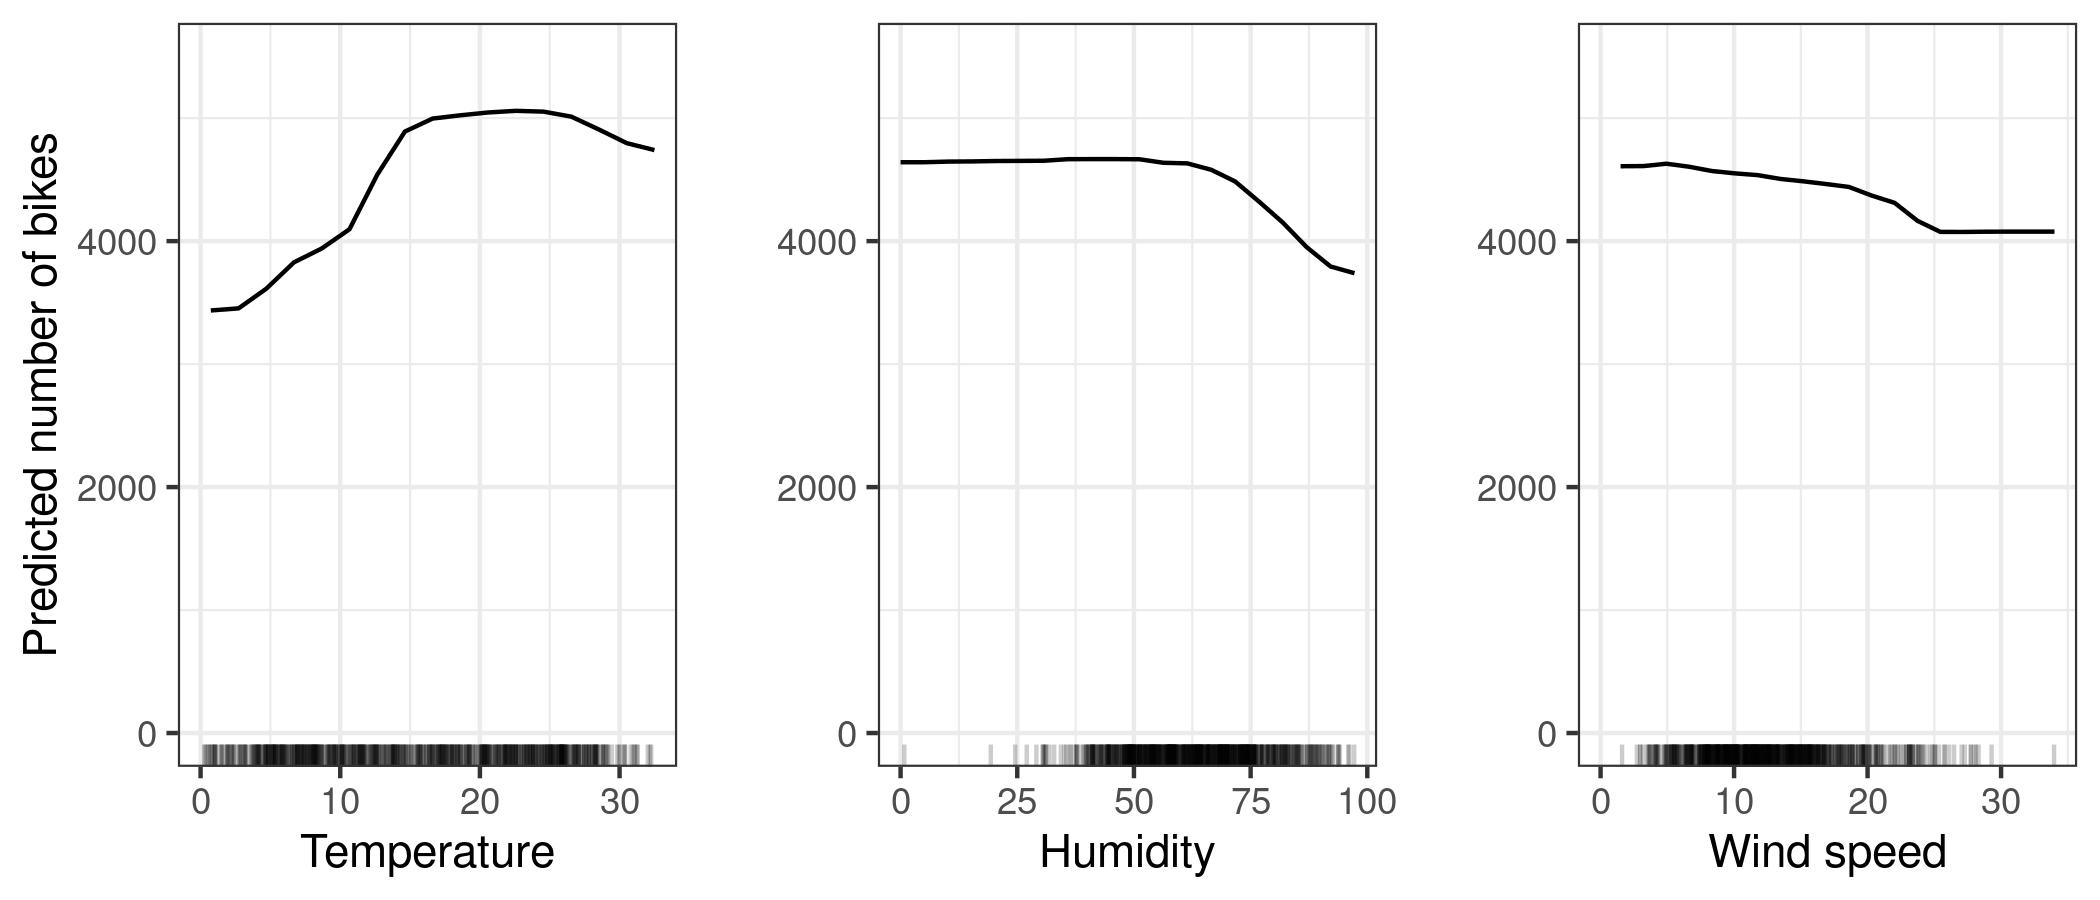
\includegraphics[width=\textwidth]{pdp-bike-1}
%      \caption{\footnotesize C. Molnar, IML book}
%    \end{figure}
%  \end{onlyenv}
%\end{frame}
%
%\begin{frame}
%  \frametitle{Issues with PDPs}
%  \begin{onlyenv}<1>
%    \begin{itemize}
%    \item The marginal distribution ignores correlated features!
%    \item To compute the effect of temperature $=33$ degrees it will (also) use an instance
%        with month = January
%    \end{itemize}
%    \begin{figure}
%      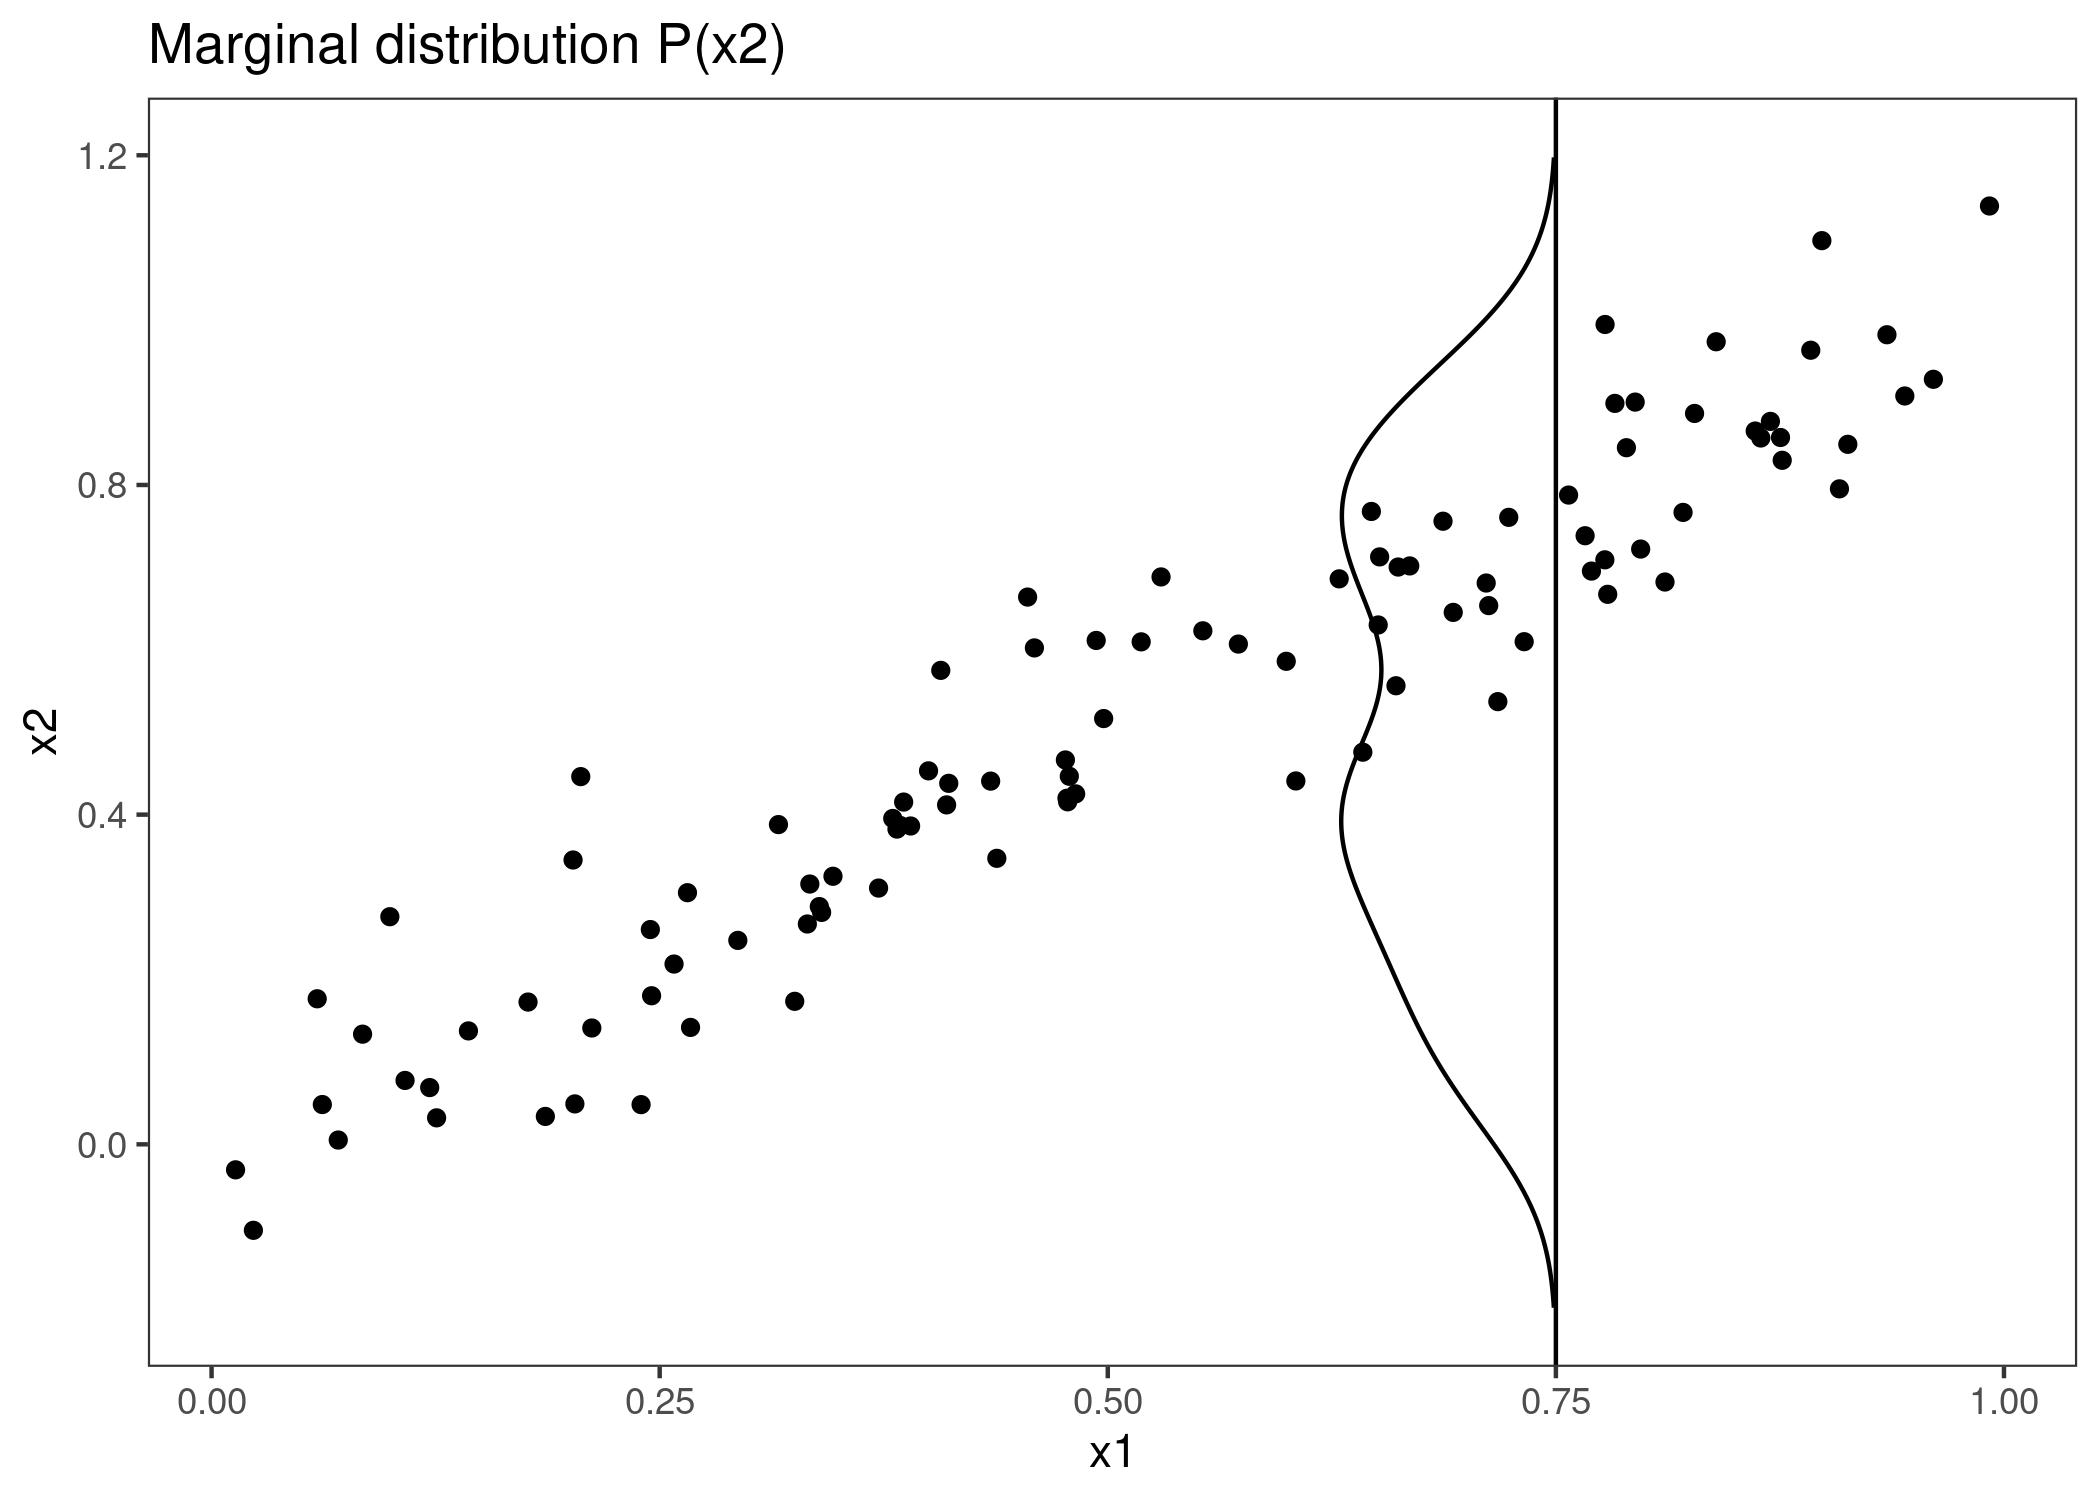
\includegraphics[width=.6\textwidth]{aleplot-motivation1-1}
%      \caption{\footnotesize C. Molnar, IML book}
%    \end{figure}
%  \end{onlyenv}
%\end{frame}
%
%
%\begin{frame}
%  \frametitle{Accumulated Local Effects (ALE)\footnote{D. Apley and
%    J. Zhu. ``Visualizing the effects of predictor variables in black box
%    supervised learning models.'' Journal of the Royal Statistical Society:
%    Series B (Statistical Methodology) 82.4 (2020): 1059-1086.}}
%
%  \begin{itemize}
%  \item Resolves problems that result from the feature correlation by computing
%    differences over a (small) window
%  \item Definition: \(f(x_s) = \int_{x_{min}}^{x_s}\mathbb{E}_{\Vx_c|z}[ \frac{\partial f}{\partial x_s}(z, \Vx_c)] \partial z\)
%  \end{itemize}
%\end{frame}
%
%\begin{frame}
%  \frametitle{ALE approximation}
%  Approximation: \(f(x_s) = \sum\limits_{k=1}^{k_x}
%  \underbrace{\frac{1}{|\mathcal{S}_k|} \sum_{i:\Vx^i \in \mathcal{S}_k}
%    \underbrace{[f(z_k, \Vx^i_c) - f(z_{k-1}, \Vx^i_c)]}_{\text{point
%        effect}}}_{\text{bin effect}} \)
%
%  \begin{figure}[ht]
%    \centering
%    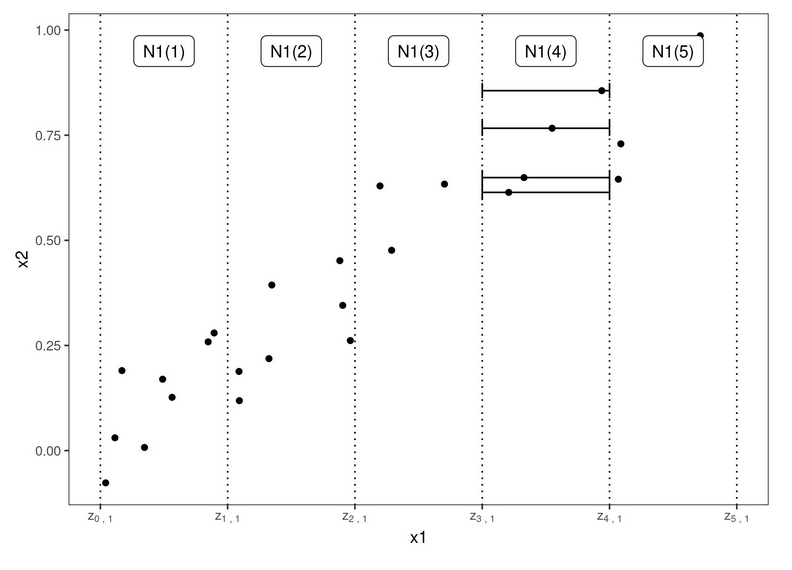
\includegraphics[width=0.65\textwidth]{./figures/ale_bins_iml.png}
%    \caption{\footnotesize C. Molnar, IML book}
%  \end{figure}
%\end{frame}
%
%\begin{frame}
%  \frametitle{ALE plots - examples}
%  \begin{figure}
%    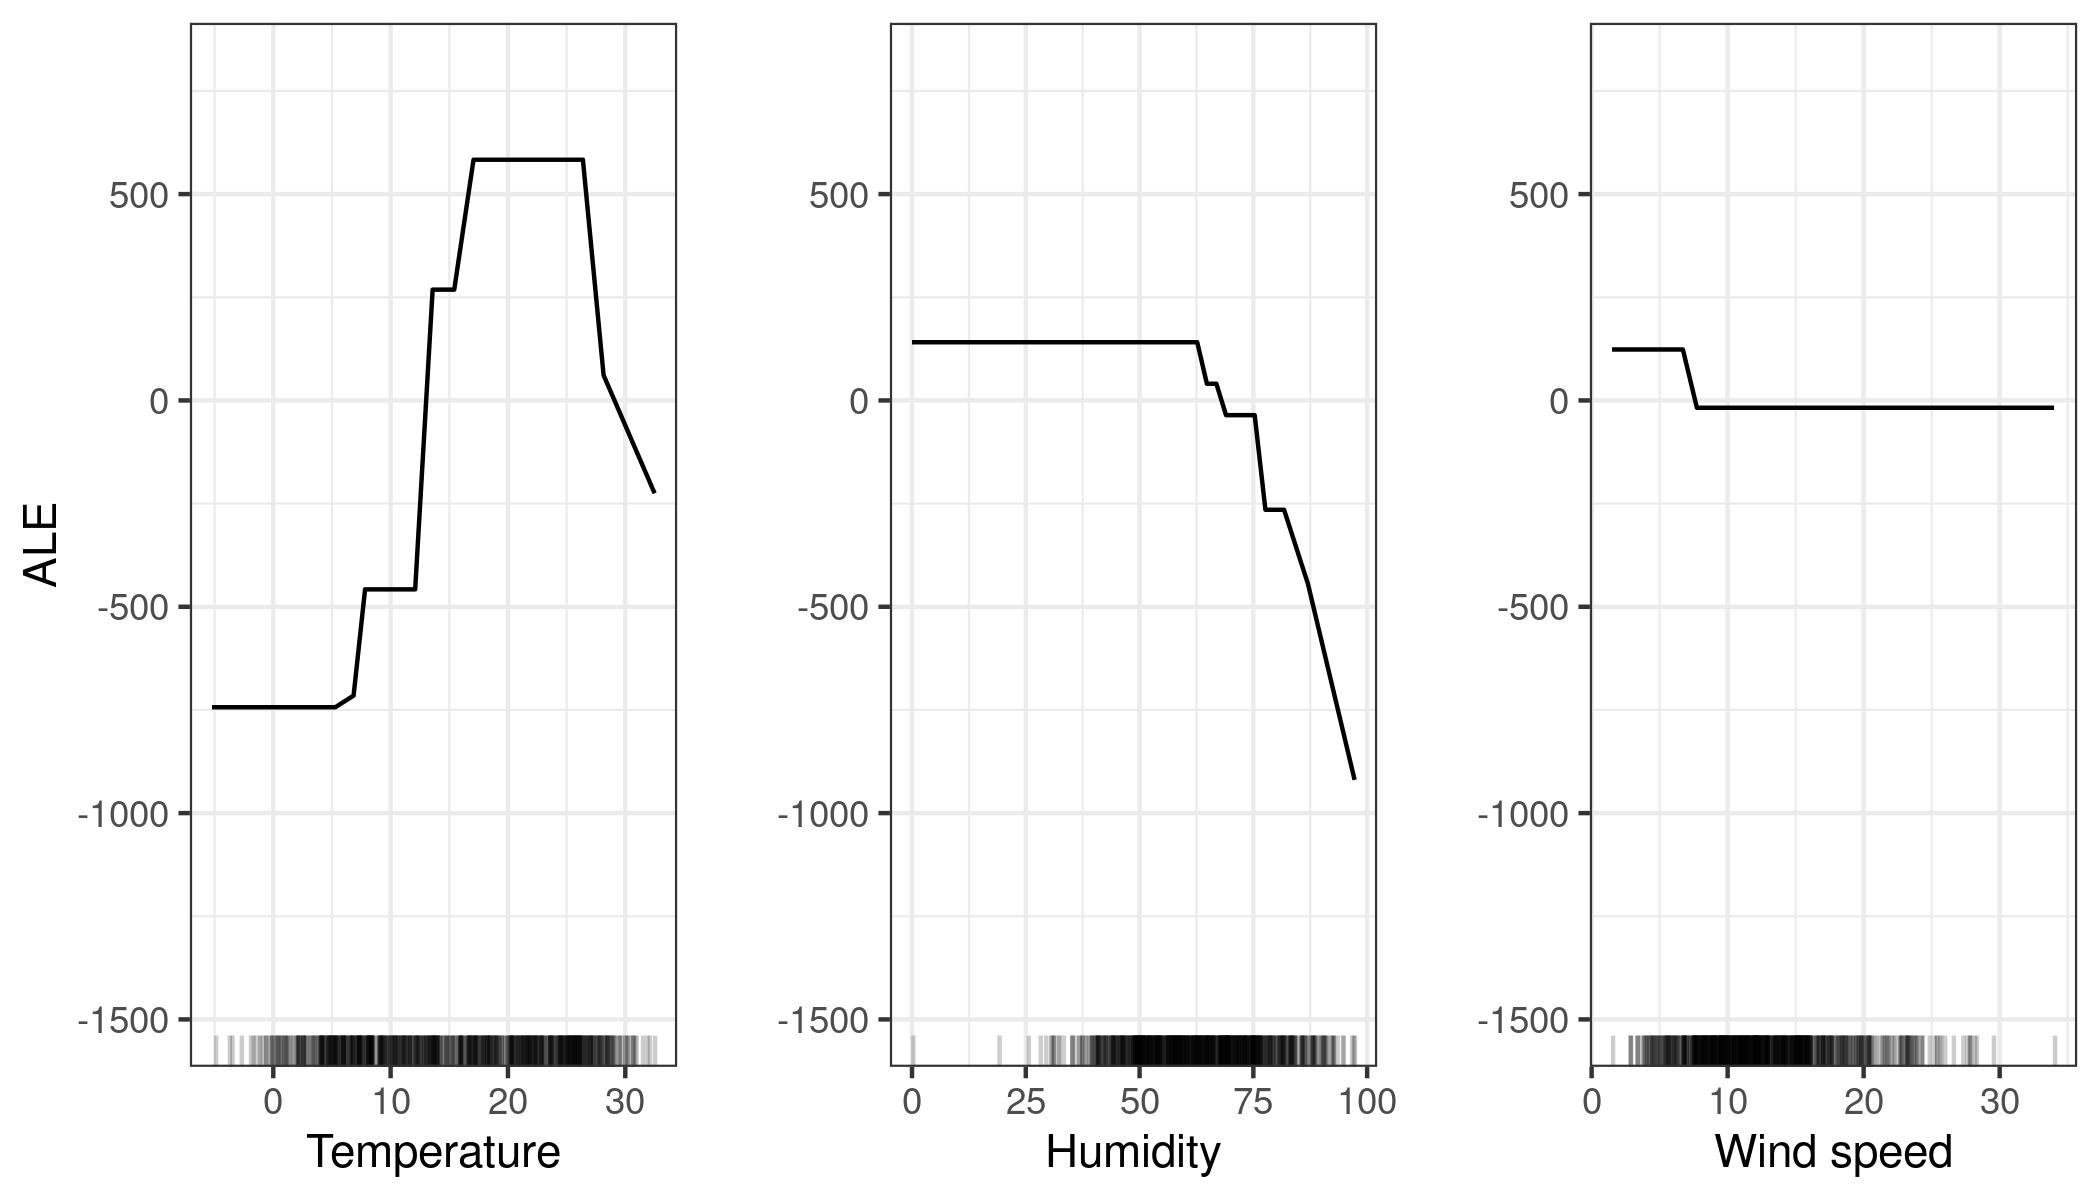
\includegraphics[width=1\textwidth]{ale-bike-1}
%    \caption{\footnotesize C. Molnar, IML book}
%  \end{figure}
%\end{frame}
